\documentclass[12pt]{extarticle}
\usepackage[paperwidth=18in,paperheight=8.5in]{geometry}
\usepackage{amsmath}
\usepackage{hyperref}
\usepackage{multirow}
\usepackage{pdfpages}
\usepackage[utf8]{inputenc}
\title{Kaon mixing: chiral and continuum extrapolations}
\author{R Mukherjee}
\date{\today}
\begin{document}
\maketitle
\tableofcontents
\clearpage
\begin{figure}
\centering
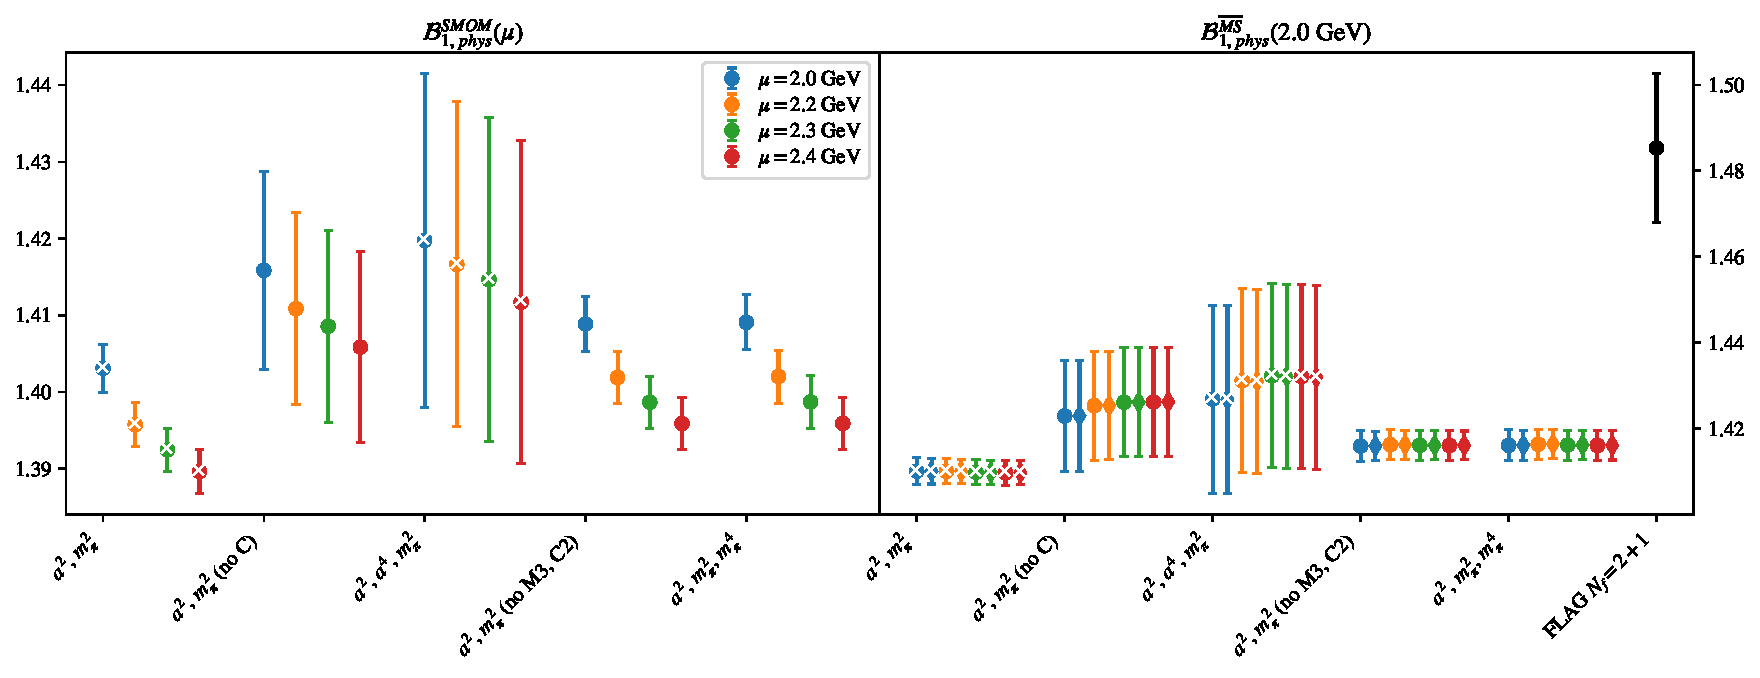
\includegraphics[page=1, width=1.1\textwidth]{VVpAA/SUSY/fit_summary_bag.pdf}
\caption{$\mathcal{B}_{1}$\\(left) $\mathcal{B}_{phys}$ in RI/SMOM scheme from fit variations (fits with $p$-value $<0.05$ marked with ``$\times$"). \\(right) $\mathcal{B}_{phys}$ in $\overline{MS}$ computed using $\mathcal{B}^{\overline{MS}} = R^{\overline{MS}\leftarrow SMOM}(2.0)\sigma_{npt}(2.0,\mu) \mathcal{B}^{SMOM}(\mu)$.}
\end{figure}
\clearpage
\begin{figure}
\centering
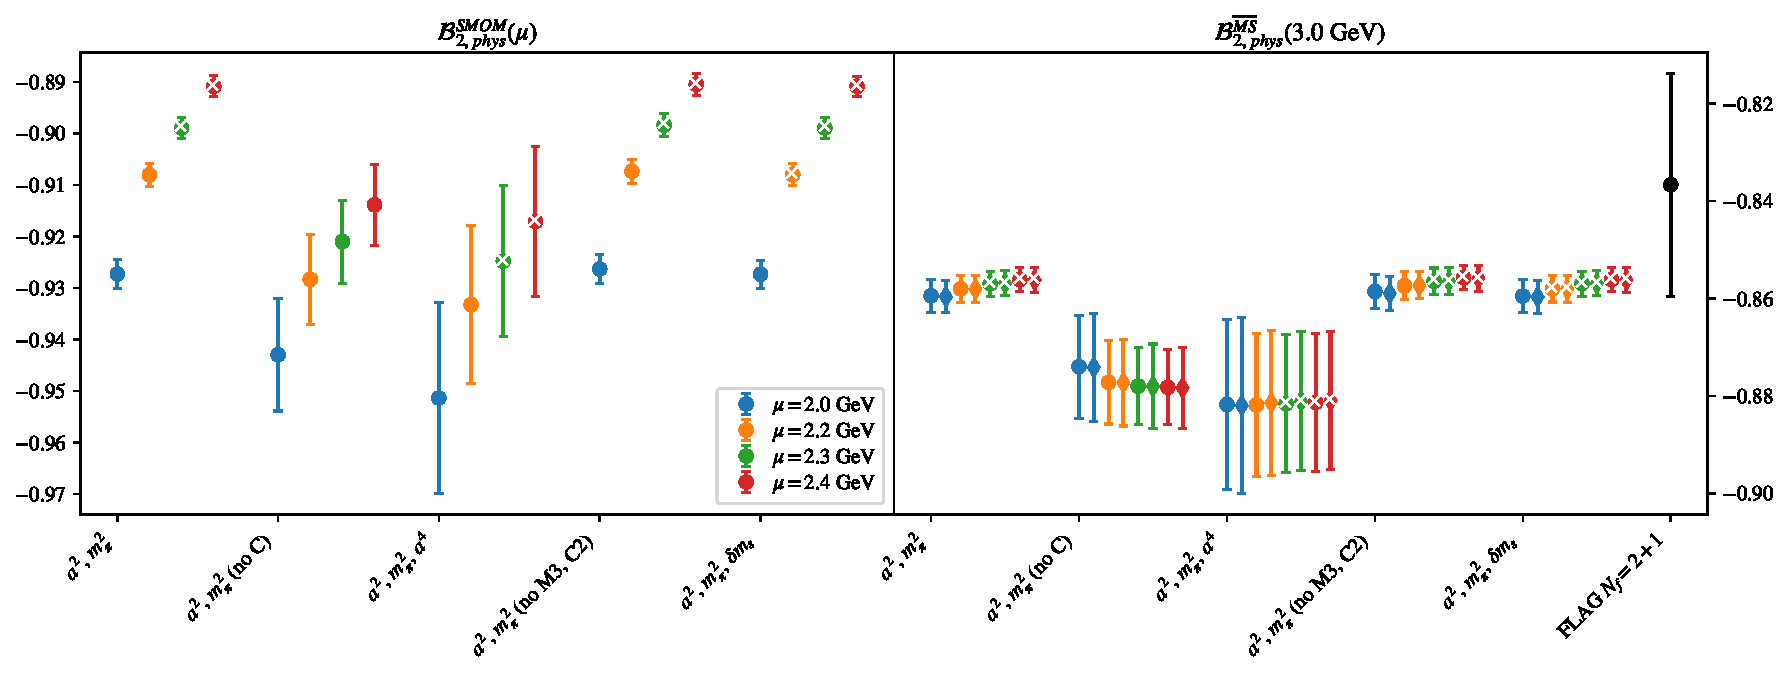
\includegraphics[page=1, width=1.1\textwidth]{VVmAA/SUSY/fit_summary_bag.pdf}
\caption{$\mathcal{B}_{2}$\\(left) $\mathcal{B}_{phys}$ in RI/SMOM scheme from fit variations (fits with $p$-value $<0.05$ marked with ``$\times$"). \\(right) $\mathcal{B}_{phys}$ in $\overline{MS}$ computed using $\mathcal{B}^{\overline{MS}} = R^{\overline{MS}\leftarrow SMOM}(3.0)\sigma_{npt}(3.0,\mu) \mathcal{B}^{SMOM}(\mu)$.}
\end{figure}
\clearpage
\begin{figure}
\centering
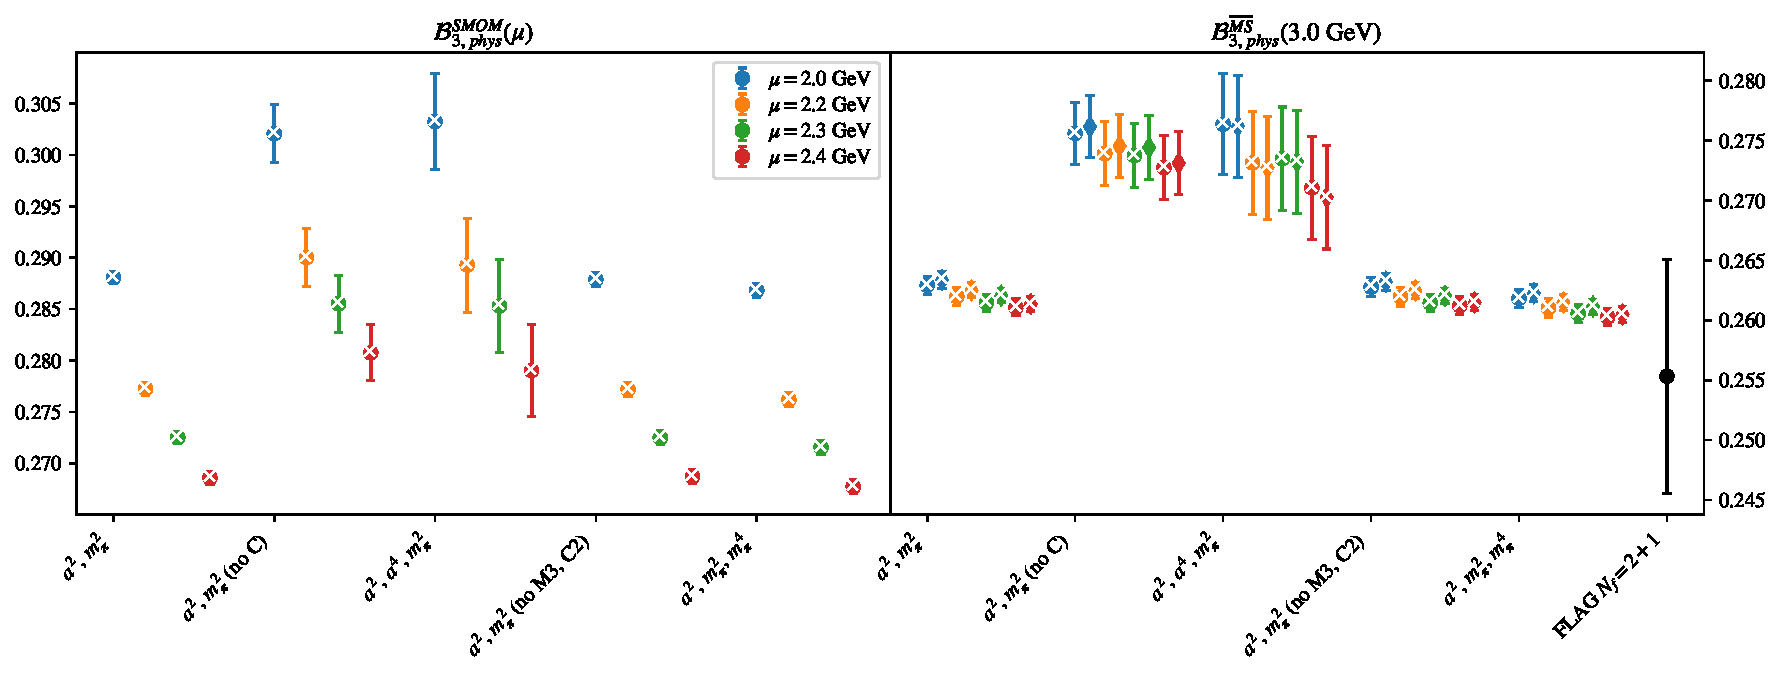
\includegraphics[page=1, width=1.1\textwidth]{SSmPP/SUSY/fit_summary_bag.pdf}
\caption{$\mathcal{B}_{3}$\\(left) $\mathcal{B}_{phys}$ in RI/SMOM scheme from fit variations (fits with $p$-value $<0.05$ marked with ``$\times$"). \\(right) $\mathcal{B}_{phys}$ in $\overline{MS}$ computed using $\mathcal{B}^{\overline{MS}} = R^{\overline{MS}\leftarrow SMOM}(3.0)\sigma_{npt}(3.0,\mu) \mathcal{B}^{SMOM}(\mu)$.}
\end{figure}
\clearpage
\begin{figure}
\centering
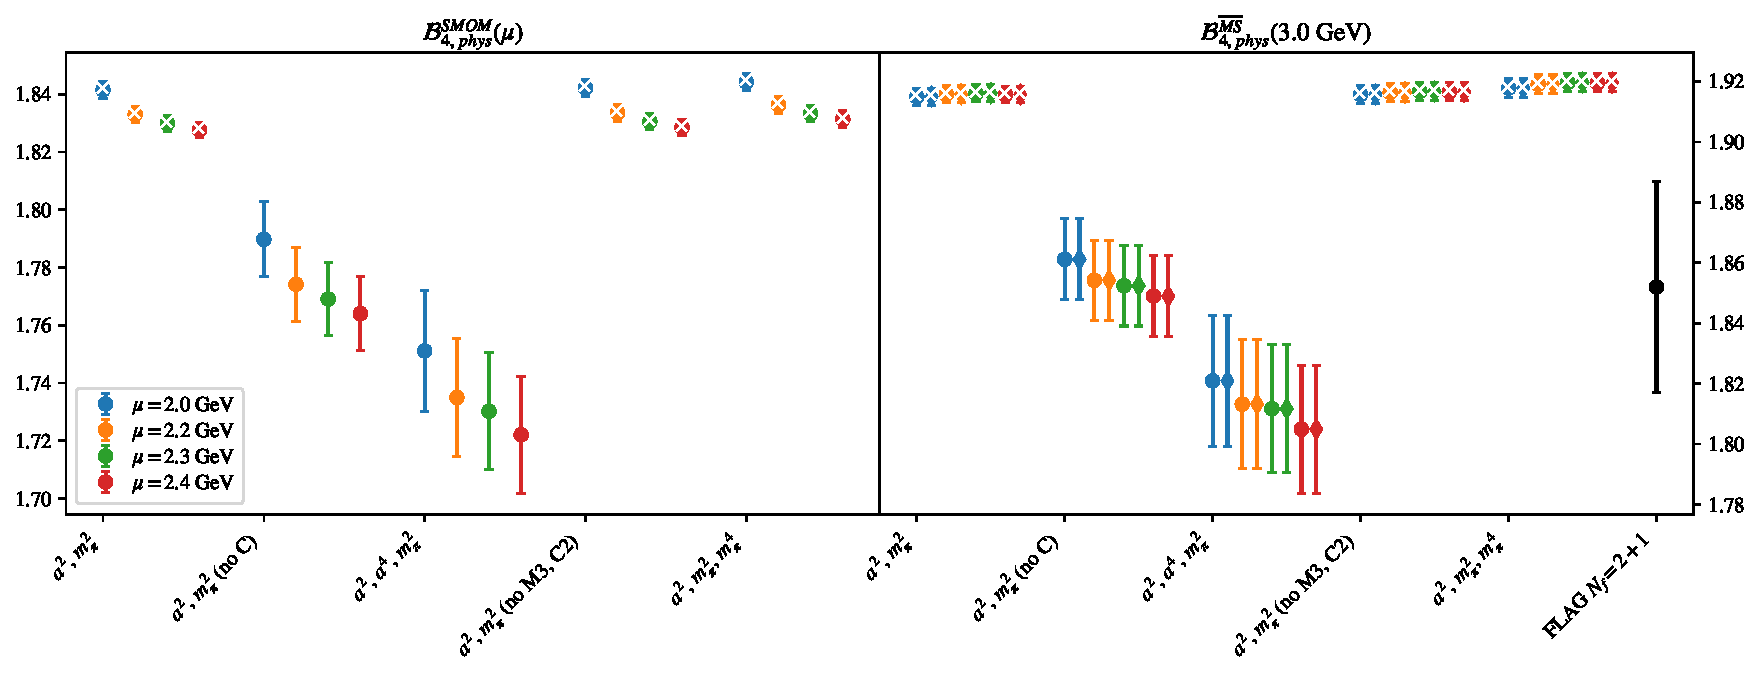
\includegraphics[page=1, width=1.1\textwidth]{SSpPP/SUSY/fit_summary_bag.pdf}
\caption{$\mathcal{B}_{4}$\\(left) $\mathcal{B}_{phys}$ in RI/SMOM scheme from fit variations (fits with $p$-value $<0.05$ marked with ``$\times$"). \\(right) $\mathcal{B}_{phys}$ in $\overline{MS}$ computed using $\mathcal{B}^{\overline{MS}} = R^{\overline{MS}\leftarrow SMOM}(3.0)\sigma_{npt}(3.0,\mu) \mathcal{B}^{SMOM}(\mu)$.}
\end{figure}
\clearpage
\begin{figure}
\centering
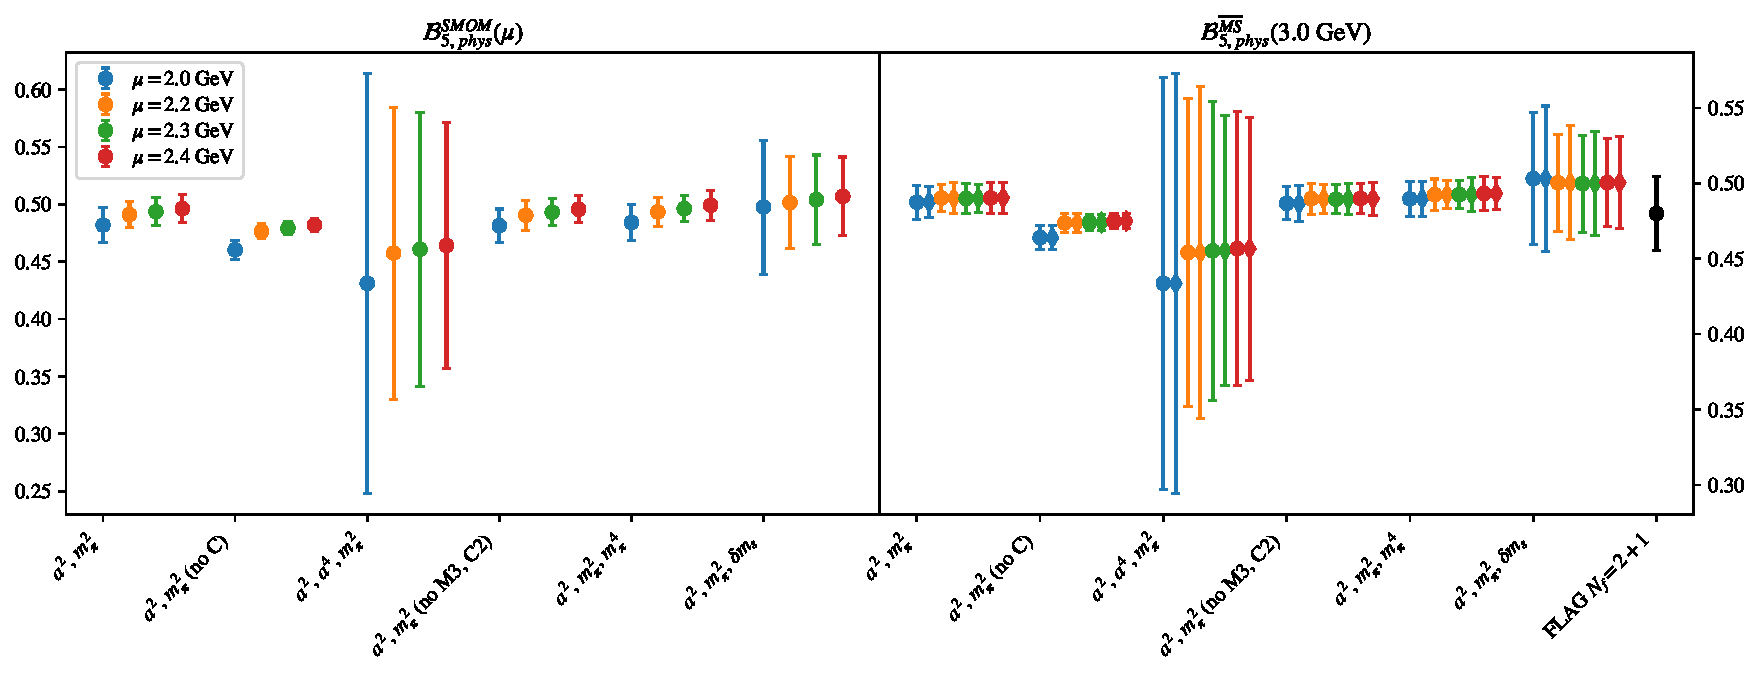
\includegraphics[page=1, width=1.1\textwidth]{TT/SUSY/fit_summary_bag.pdf}
\caption{$\mathcal{B}_{5}$\\(left) $\mathcal{B}_{phys}$ in RI/SMOM scheme from fit variations (fits with $p$-value $<0.05$ marked with ``$\times$"). \\(right) $\mathcal{B}_{phys}$ in $\overline{MS}$ computed using $\mathcal{B}^{\overline{MS}} = R^{\overline{MS}\leftarrow SMOM}(3.0)\sigma_{npt}(3.0,\mu) \mathcal{B}^{SMOM}(\mu)$.}
\end{figure}
\clearpage
\section{$\mathcal{B}_1$}
\begin{table}[h!]
\begin{center}
\begin{tabular}{|c|c|c|c|c|c|c|}
\hline
$\mu$ (GeV) & $a^2$, $m_\pi^2$& $a^2$, $m_\pi^2$ (no C)& $a^2$, $m_\pi^2$, $a^4$& $a^2$, $m_\pi^2$ (no M3, C2)& $a^2$, $m_\pi^2$, $m_\pi^4$& $a^2$, $m_\pi^2$, $\delta m_s$\\
\hline
2.0& \hyperlink{VVpAA/SUSY/a2m2_20.pdf.1}{\textbf{1.4032(27)}: 1.885 (0.093)} & \hyperlink{VVpAA/SUSY/a2m2noC_20.pdf.1}{\textbf{1.414(13)}: 0.924 (0.397)} & \hyperlink{VVpAA/SUSY/a2a4m2_20.pdf.1}{\textbf{1.419(21)}: 2.182 (0.068)} & \hyperlink{VVpAA/SUSY/a2m2mcut_20.pdf.1}{\textbf{1.4071(37)}: 0.267 (0.849)} & \hyperlink{VVpAA/SUSY/a2m2m4_20.pdf.1}{\textbf{1.4079(35)}: 0.705 (0.588)} & \hyperlink{VVpAA/SUSY/a2m2delm_20.pdf.1}{\textbf{1.4015(31)}: 1.892 (0.109)}\\
2.2& \hyperlink{VVpAA/SUSY/a2m2_22.pdf.1}{\textbf{1.3957(27)}: 2.22 (0.049)} & \hyperlink{VVpAA/SUSY/a2m2noC_22.pdf.1}{\textbf{1.409(12)}: 1.166 (0.312)} & \hyperlink{VVpAA/SUSY/a2a4m2_22.pdf.1}{\textbf{1.415(21)}: 2.528 (0.039)} & \hyperlink{VVpAA/SUSY/a2m2mcut_22.pdf.1}{\textbf{1.4000(37)}: 0.365 (0.779)} & \hyperlink{VVpAA/SUSY/a2m2m4_22.pdf.1}{\textbf{1.4007(35)}: 0.929 (0.446)} & \hyperlink{VVpAA/SUSY/a2m2delm_22.pdf.1}{\textbf{1.3938(31)}: 2.149 (0.072)}\\
2.3& \hyperlink{VVpAA/SUSY/a2m2_23.pdf.1}{\textbf{1.3924(27)}: 2.311 (0.041)} & \hyperlink{VVpAA/SUSY/a2m2noC_23.pdf.1}{\textbf{1.406(12)}: 1.213 (0.297)} & \hyperlink{VVpAA/SUSY/a2a4m2_23.pdf.1}{\textbf{1.413(21)}: 2.608 (0.034)} & \hyperlink{VVpAA/SUSY/a2m2mcut_23.pdf.1}{\textbf{1.3967(37)}: 0.416 (0.742)} & \hyperlink{VVpAA/SUSY/a2m2m4_23.pdf.1}{\textbf{1.3975(35)}: 0.998 (0.407)} & \hyperlink{VVpAA/SUSY/a2m2delm_23.pdf.1}{\textbf{1.3903(30)}: 2.194 (0.067)}\\
2.4& \hyperlink{VVpAA/SUSY/a2m2_24.pdf.1}{\textbf{1.3896(27)}: 2.359 (0.038)} & \hyperlink{VVpAA/SUSY/a2m2noC_24.pdf.1}{\textbf{1.404(12)}: 1.237 (0.29)} & \hyperlink{VVpAA/SUSY/a2a4m2_24.pdf.1}{\textbf{1.410(21)}: 2.669 (0.03)} & \hyperlink{VVpAA/SUSY/a2m2mcut_24.pdf.1}{\textbf{1.3940(37)}: 0.417 (0.741)} & \hyperlink{VVpAA/SUSY/a2m2m4_24.pdf.1}{\textbf{1.3947(35)}: 1.014 (0.398)} & \hyperlink{VVpAA/SUSY/a2m2delm_24.pdf.1}{\textbf{1.3875(30)}: 2.242 (0.062)}\\
\hline
\end{tabular}
\caption{Physical point value from chiral and continuum extrapolation at renormalisation scale $\mu$. Entries are \textbf{value(error)}: $\chi^2/\text{DOF}$ ($p$-value).}
\end{center}
\end{table}
\begin{table}[h!]
\begin{center}
\begin{tabular}{|c c|c|c|c|c|c|c|}
\hline
$\mu$ (GeV) &  & $a^2$, $m_\pi^2$& $a^2$, $m_\pi^2$ (no C)& $a^2$, $m_\pi^2$, $a^4$& $a^2$, $m_\pi^2$ (no M3, C2)& $a^2$, $m_\pi^2$, $m_\pi^4$& $a^2$, $m_\pi^2$, $\delta m_s$\\
\hline
\multirow{3}{0.5in}{2.0} & $\alpha$ & 0.100(10)& 0.057(55)& -0.005& 0.091(13)& 0.089(11)& 0.104(10)\\
 & $\beta$ & 0.00264(15)& 0.00238(31)& 0.00266(15)& 0.00206(34)& 0.00063(93)& 0.00273(17)\\
 & $\gamma$ &  &  & 0.21(28)&  & 0.000174(79)& -0.002(23)\\
\hline
\multirow{3}{0.5in}{2.2} & $\alpha$ & 0.104(10)& 0.051(54)& -0.024& 0.094(13)& 0.093(11)& 0.109(10)\\
 & $\beta$ & 0.00262(14)& 0.00233(30)& 0.00265(15)& 0.00199(32)& 0.00051(93)& 0.00273(16)\\
 & $\gamma$ &  &  & 0.26(27)&  & 0.000183(79)& -0.003(23)\\
\hline
\multirow{3}{0.5in}{2.3} & $\alpha$ & 0.106(10)& 0.049(54)& -0.033& 0.096(13)& 0.094(11)& 0.111(10)\\
 & $\beta$ & 0.00263(15)& 0.00233(30)& 0.00266(15)& 0.00198(32)& 0.00050(93)& 0.00274(16)\\
 & $\gamma$ &  &  & 0.28(27)&  & 0.000185(79)& -0.003(23)\\
\hline
\multirow{3}{0.5in}{2.4} & $\alpha$ & 0.107(10)& 0.049(54)& -0.031& 0.096(13)& 0.095(11)& 0.112(10)\\
 & $\beta$ & 0.00264(15)& 0.00233(30)& 0.00267(15)& 0.00199(33)& 0.00050(94)& 0.00276(16)\\
 & $\gamma$ &  &  & 0.27(27)&  & 0.000186(80)& -0.003(23)\\
\hline
\end{tabular}
\caption{Fit values of coefficients in $Q = Q_{phys} + \mathbf{\alpha} a^2 + \mathbf{\beta}\left(\frac{m_\pi^2}{f_\pi^2}-\frac{m_{\pi,PDG}^2}{f_\pi^2}\right) + \gamma(\ldots)$}
\end{center}
\end{table}
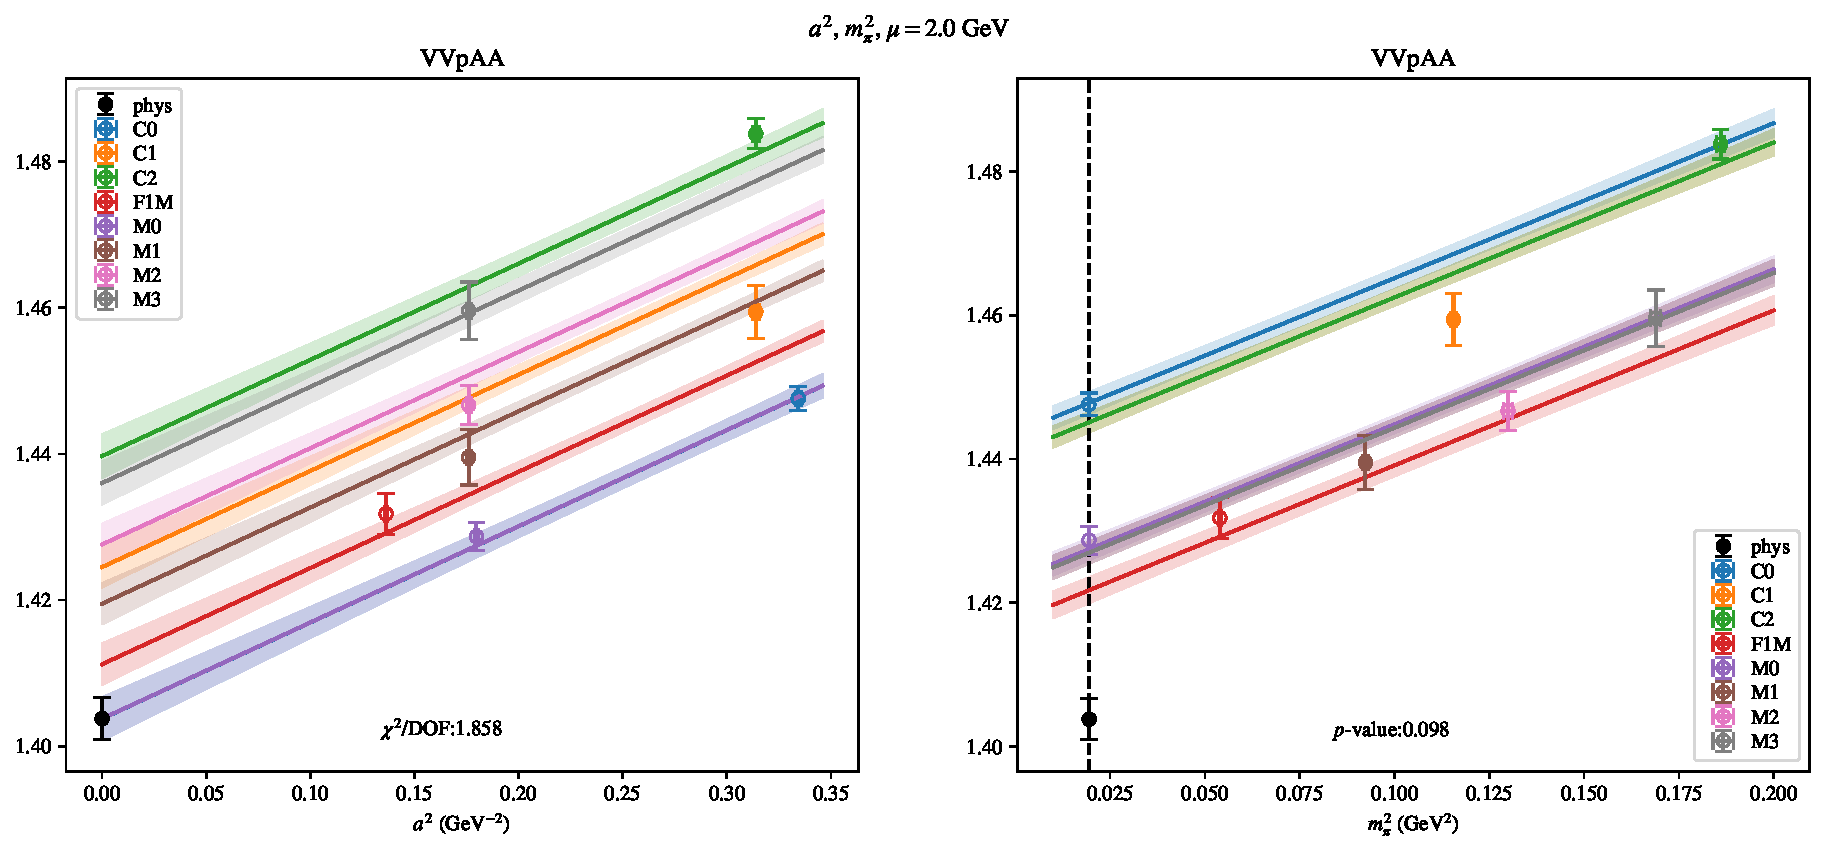
\includepdf[link, pages=-]{VVpAA/SUSY/a2m2_20.pdf}
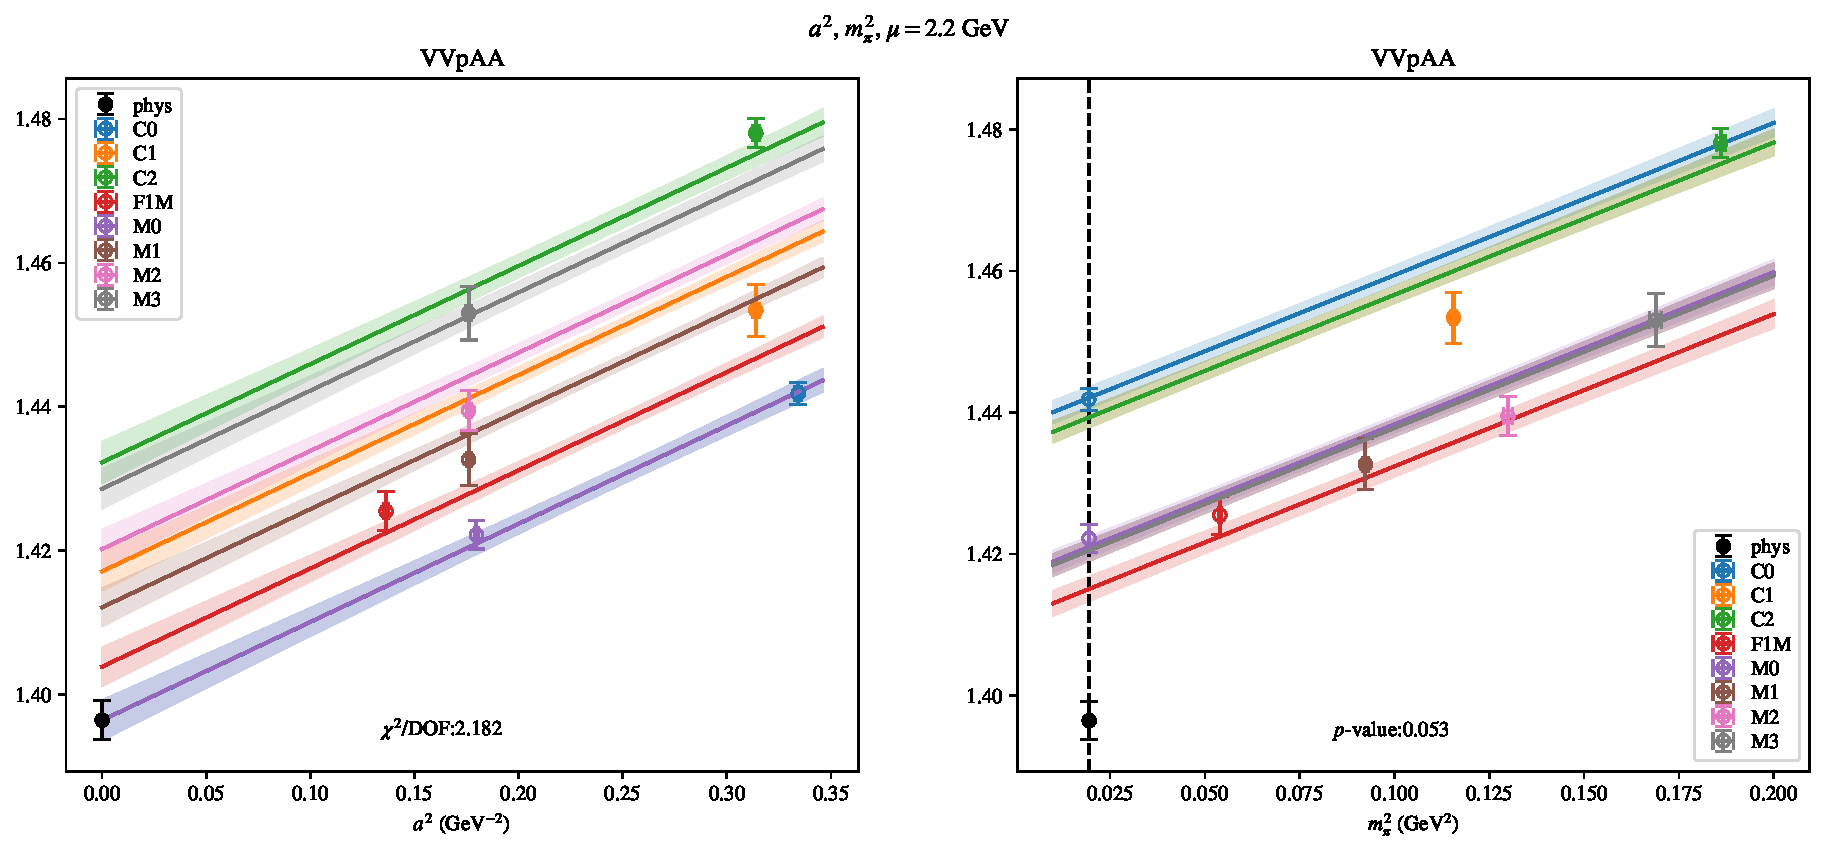
\includepdf[link, pages=-]{VVpAA/SUSY/a2m2_22.pdf}
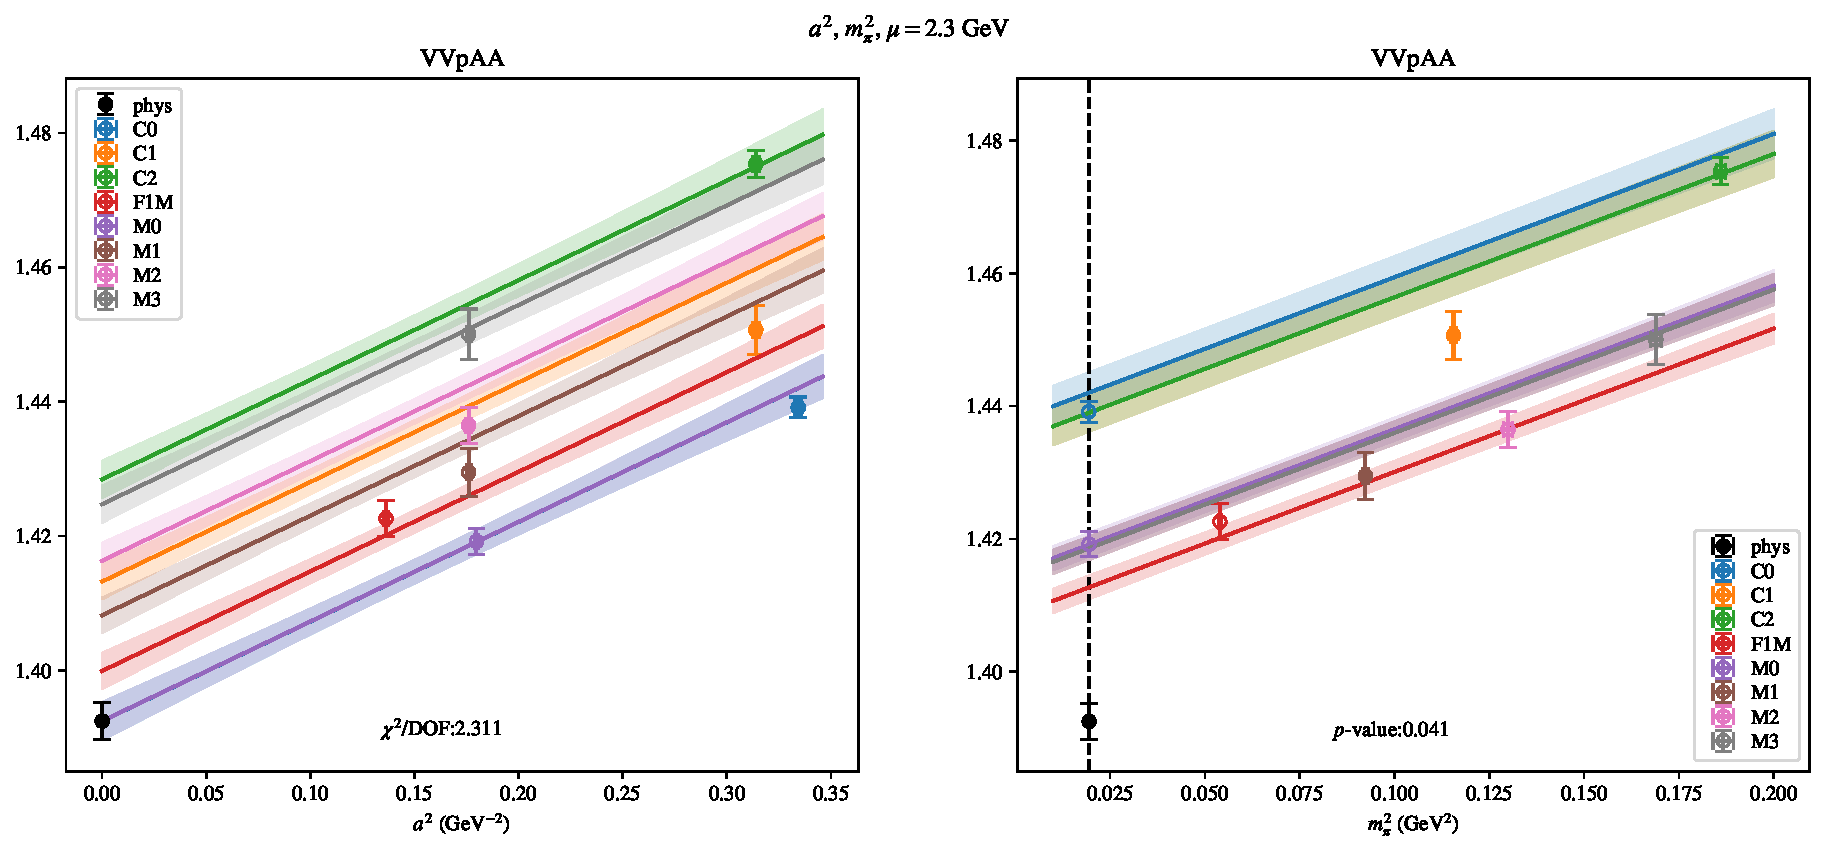
\includepdf[link, pages=-]{VVpAA/SUSY/a2m2_23.pdf}
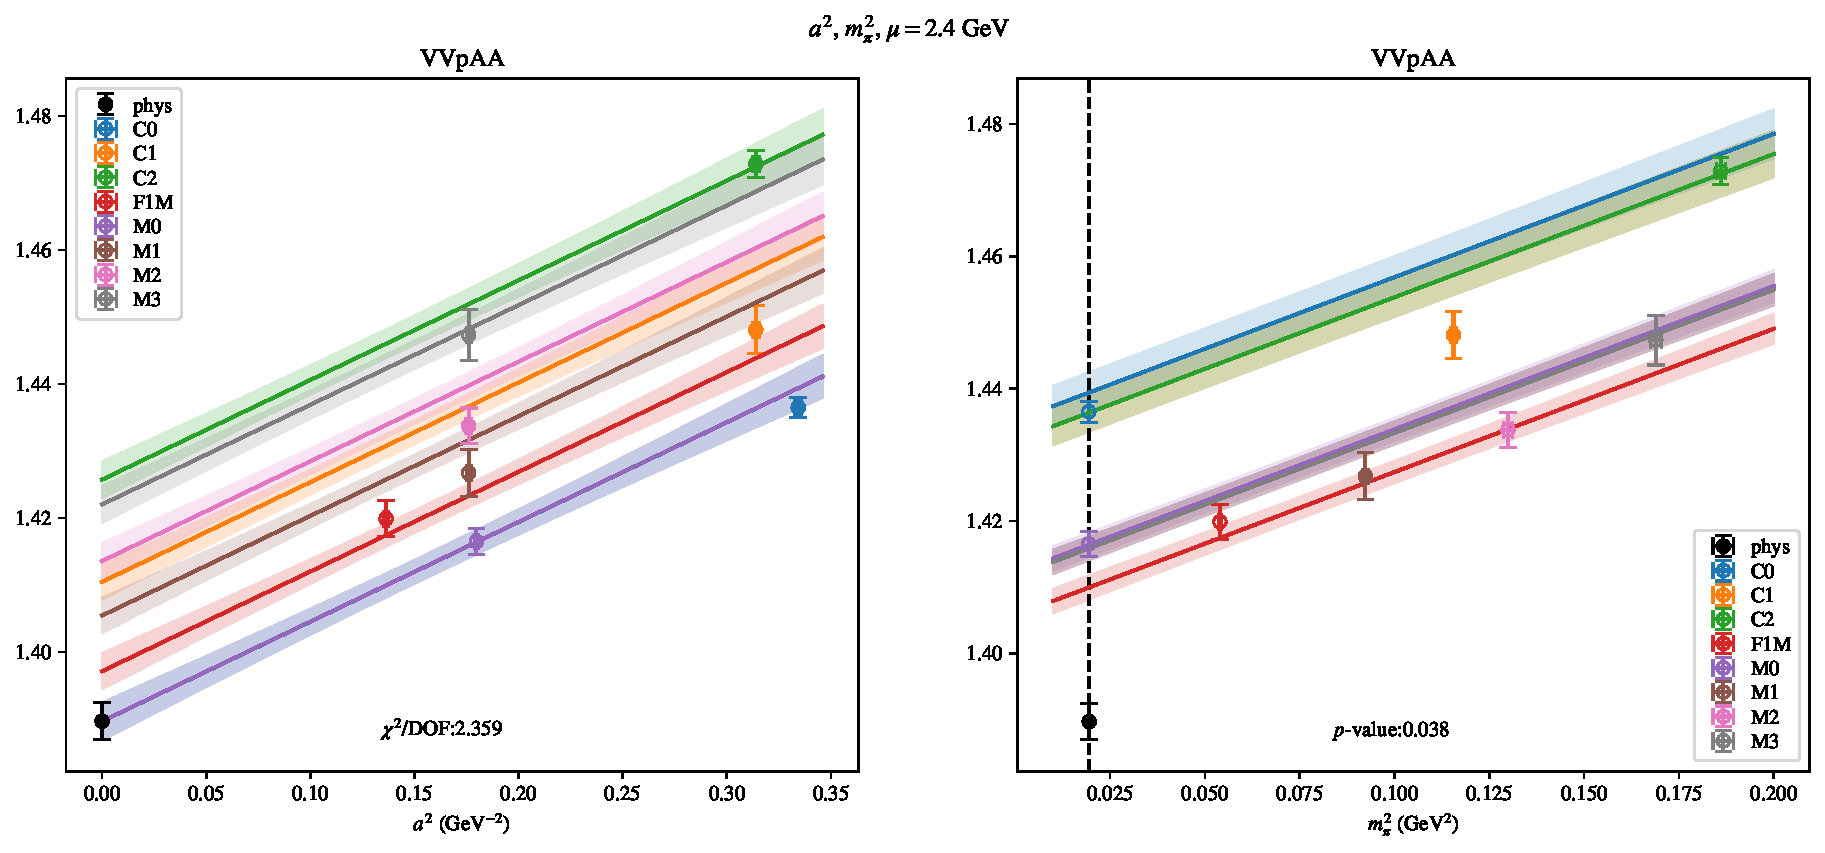
\includepdf[link, pages=-]{VVpAA/SUSY/a2m2_24.pdf}
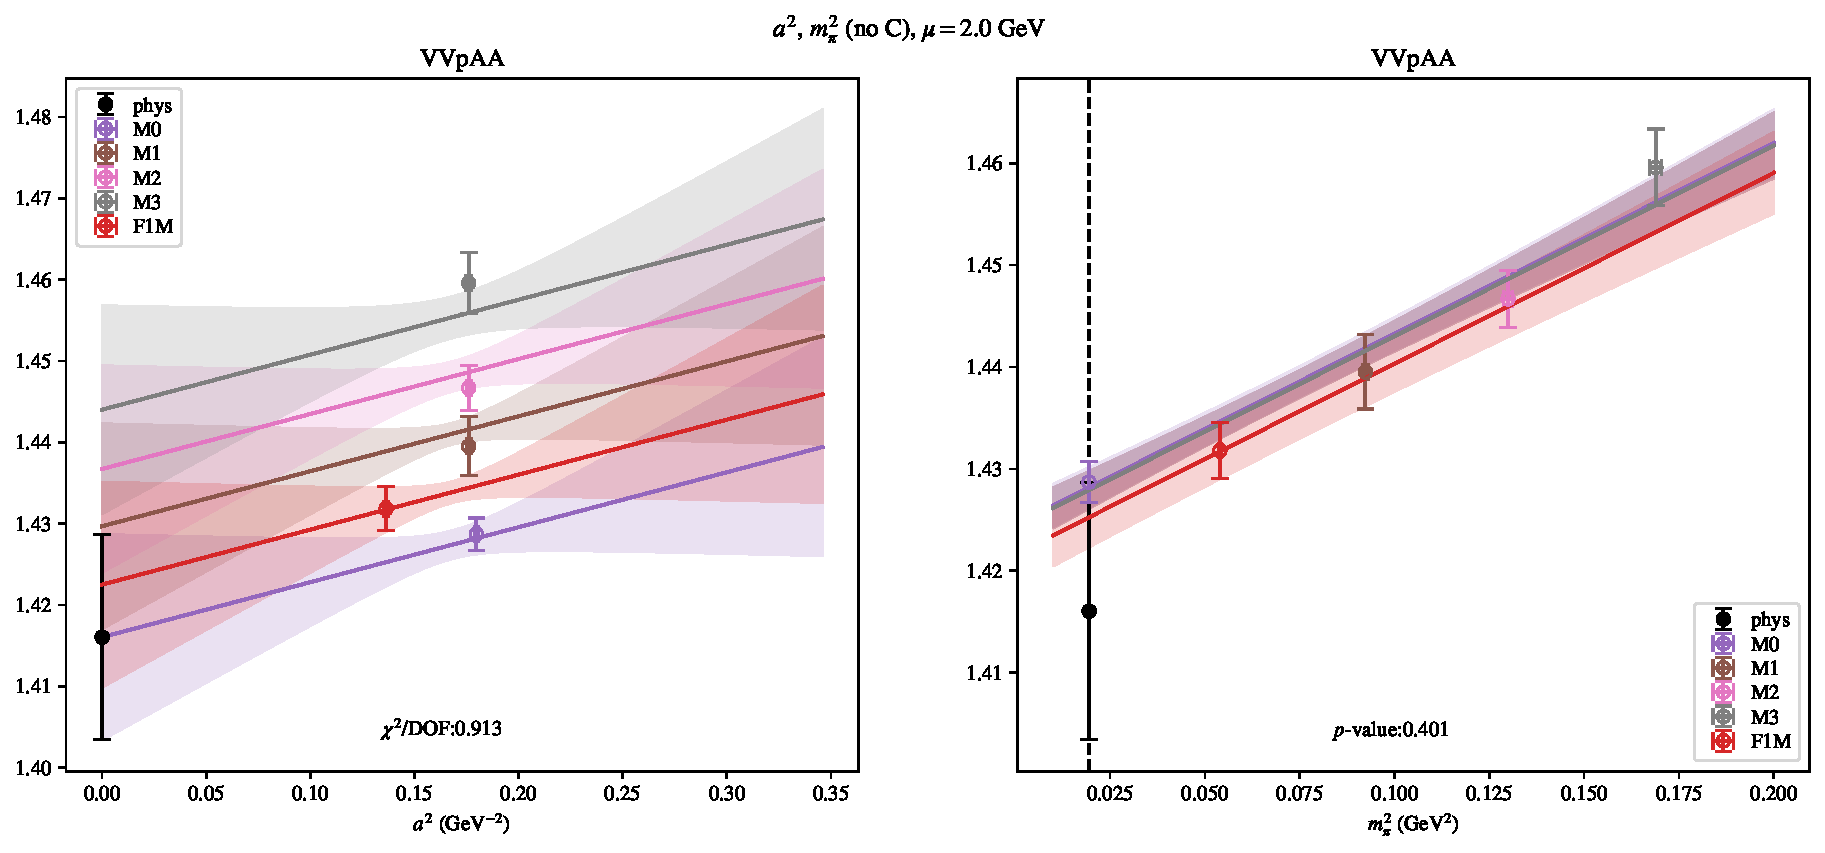
\includepdf[link, pages=-]{VVpAA/SUSY/a2m2noC_20.pdf}
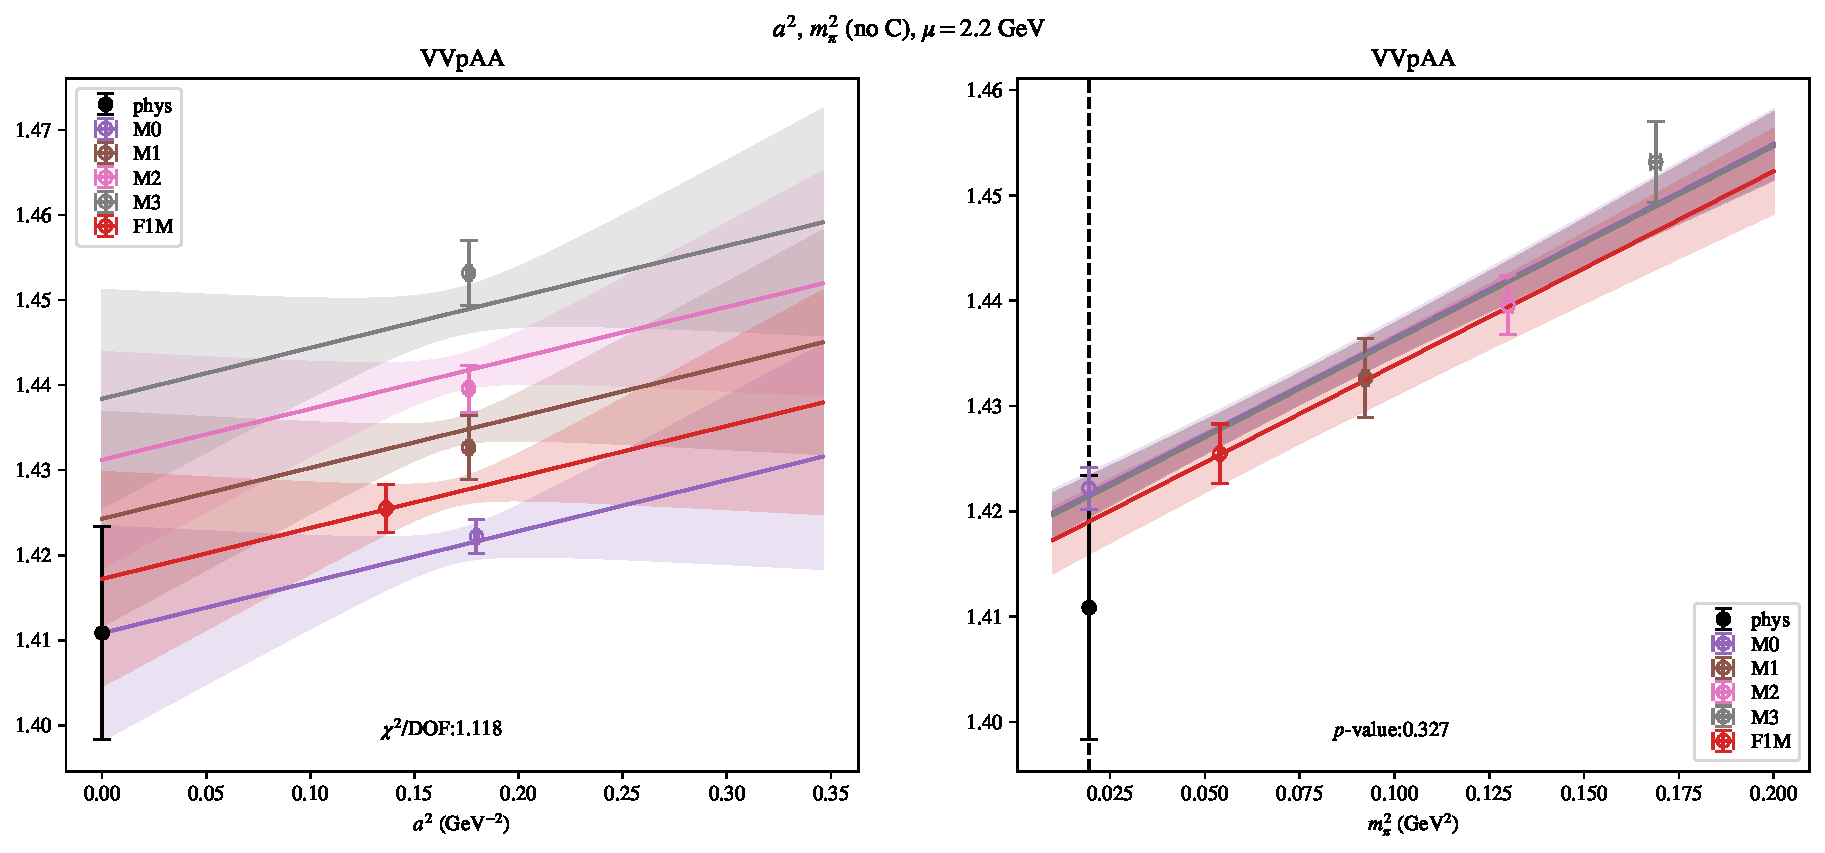
\includepdf[link, pages=-]{VVpAA/SUSY/a2m2noC_22.pdf}
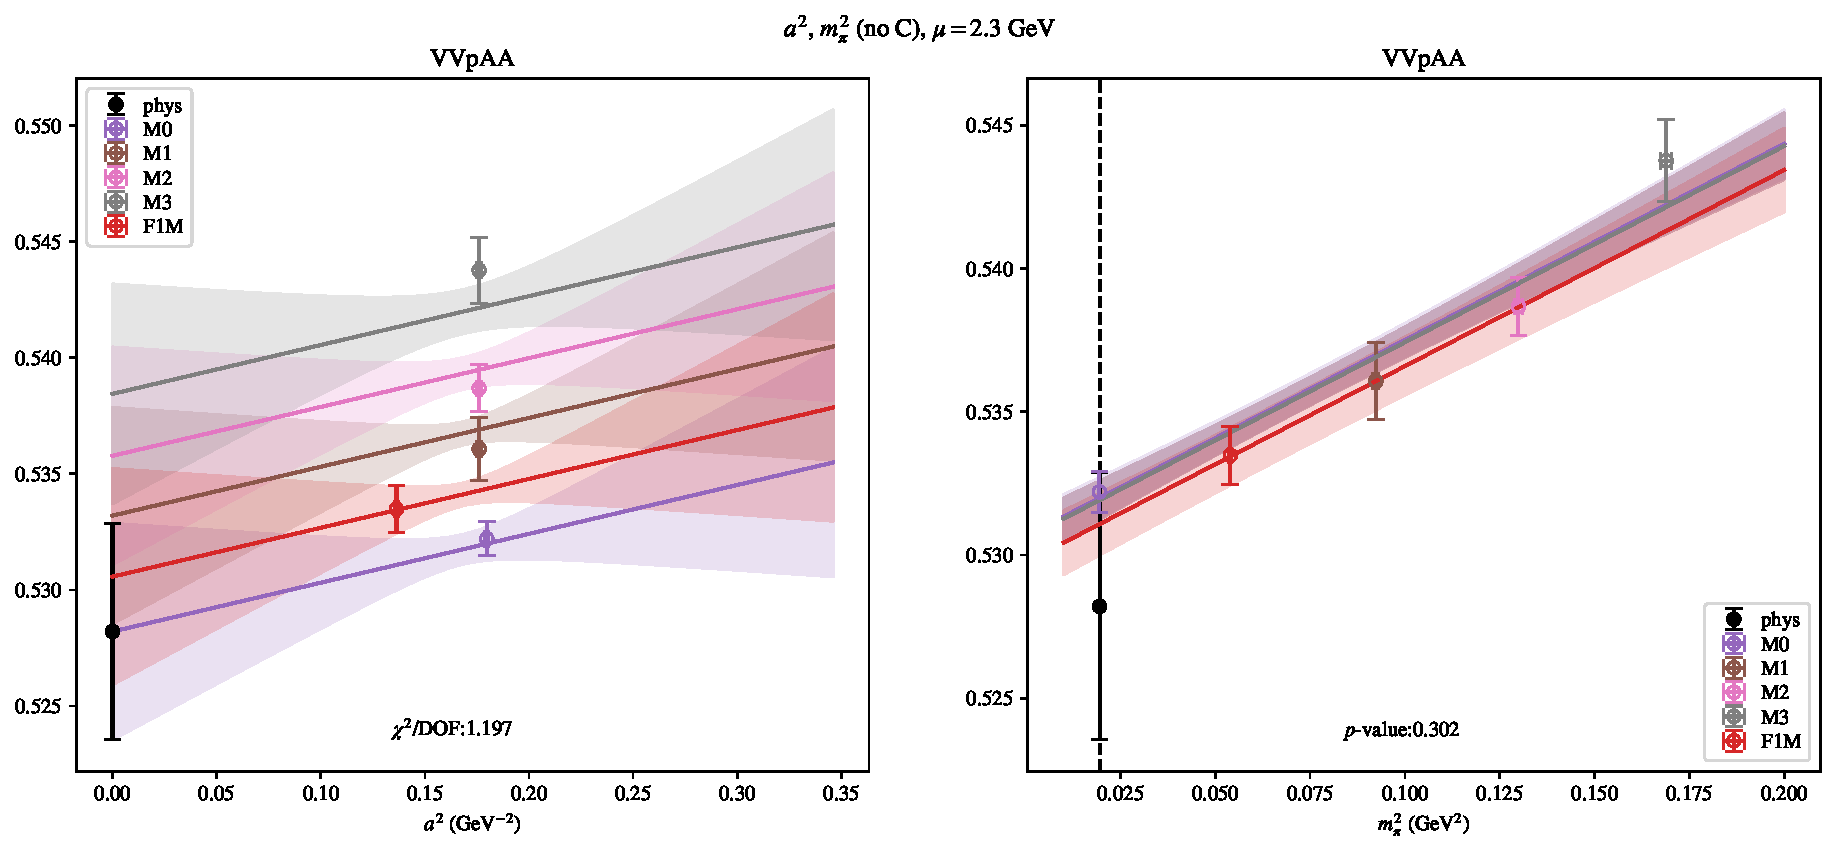
\includepdf[link, pages=-]{VVpAA/SUSY/a2m2noC_23.pdf}
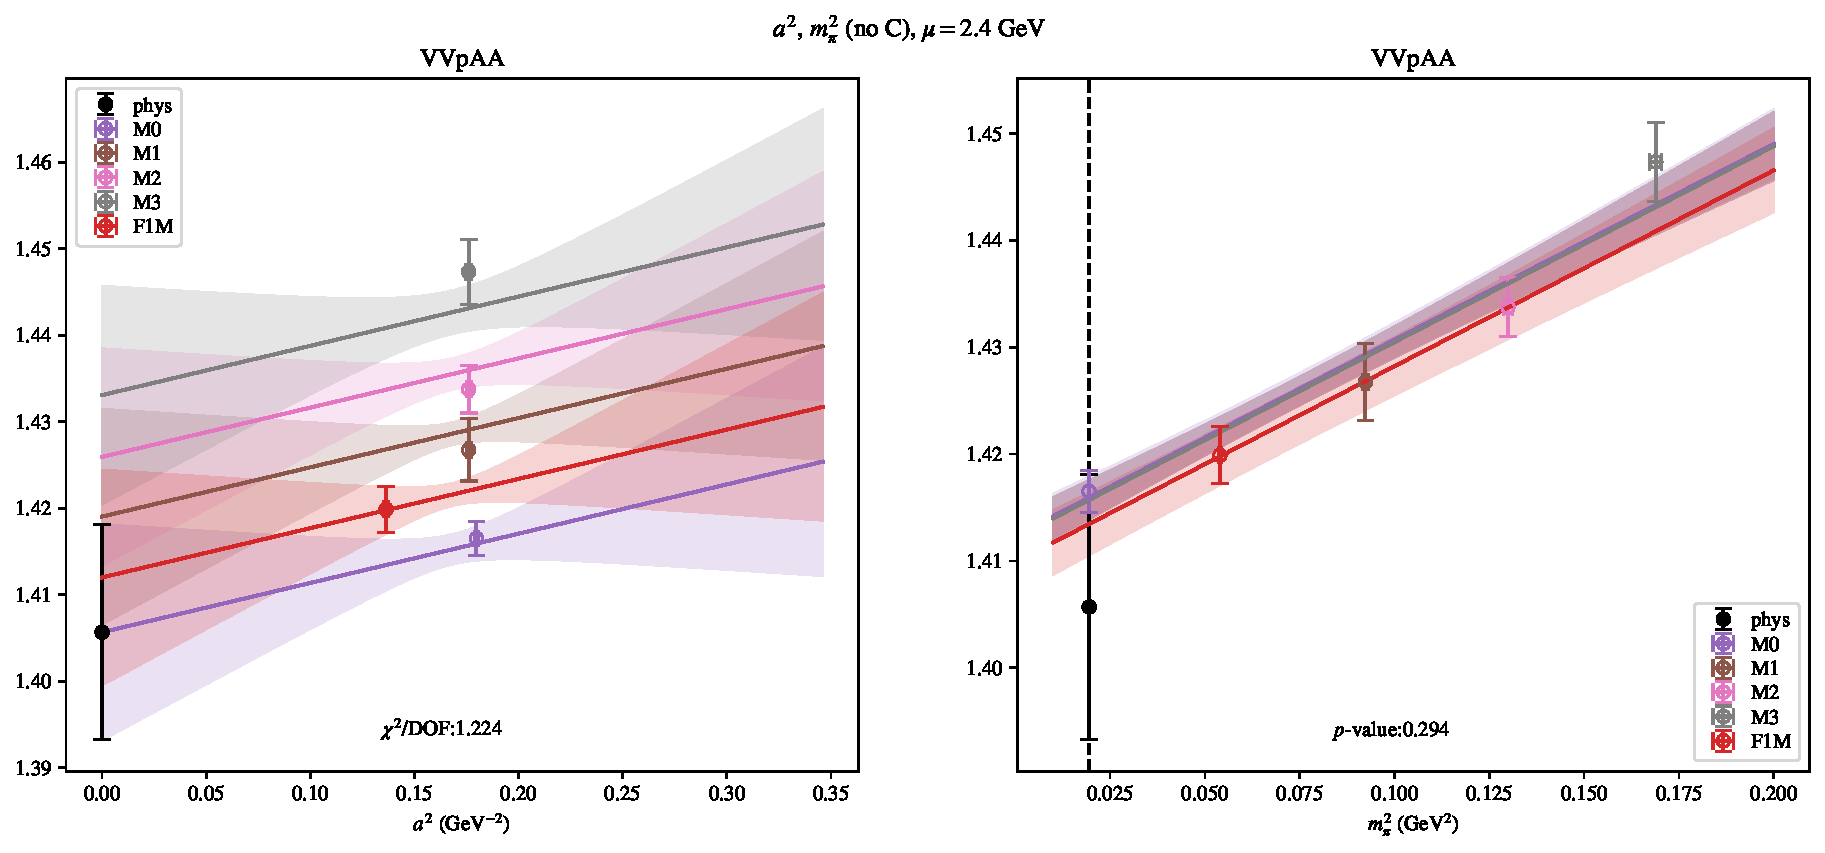
\includepdf[link, pages=-]{VVpAA/SUSY/a2m2noC_24.pdf}
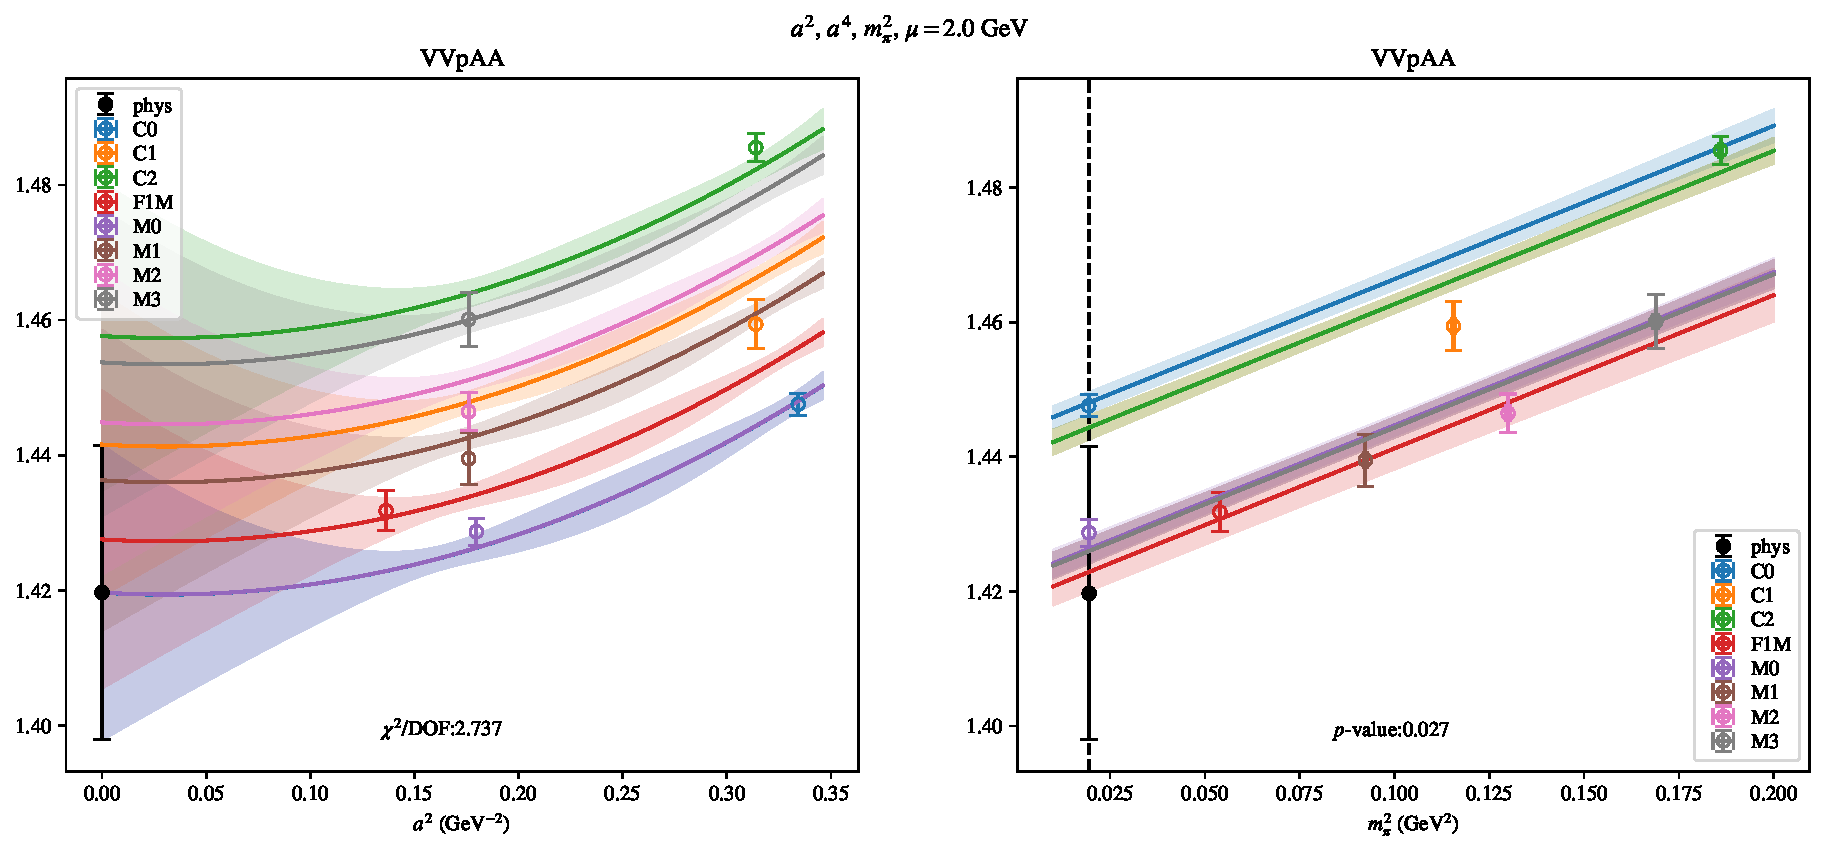
\includepdf[link, pages=-]{VVpAA/SUSY/a2a4m2_20.pdf}
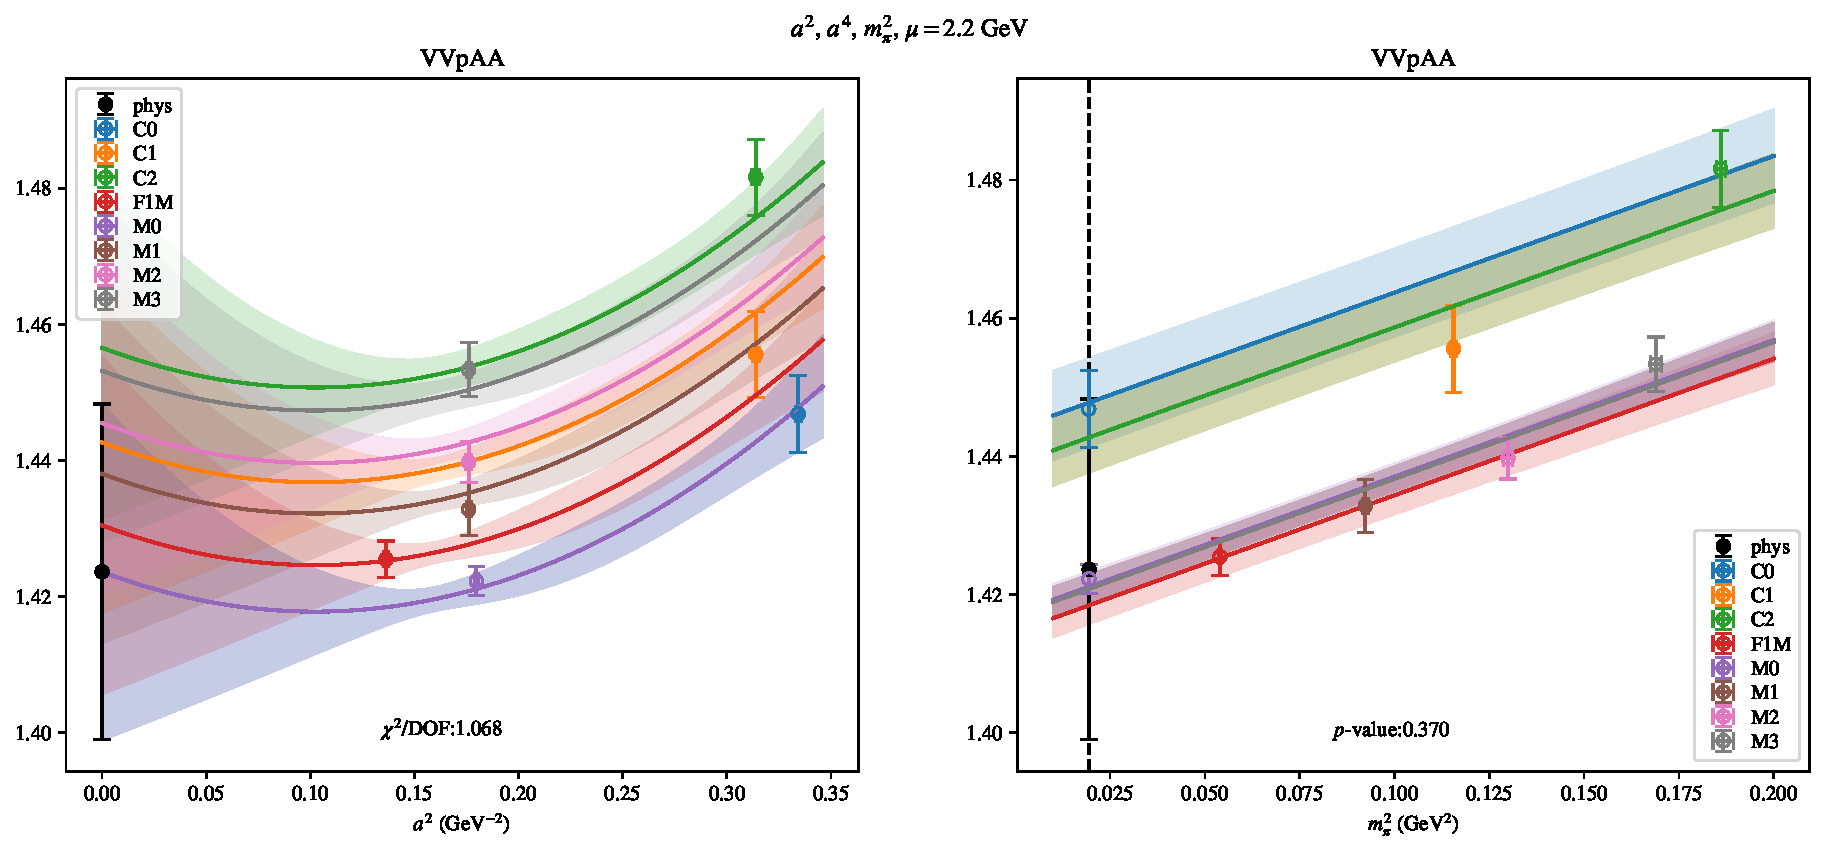
\includepdf[link, pages=-]{VVpAA/SUSY/a2a4m2_22.pdf}
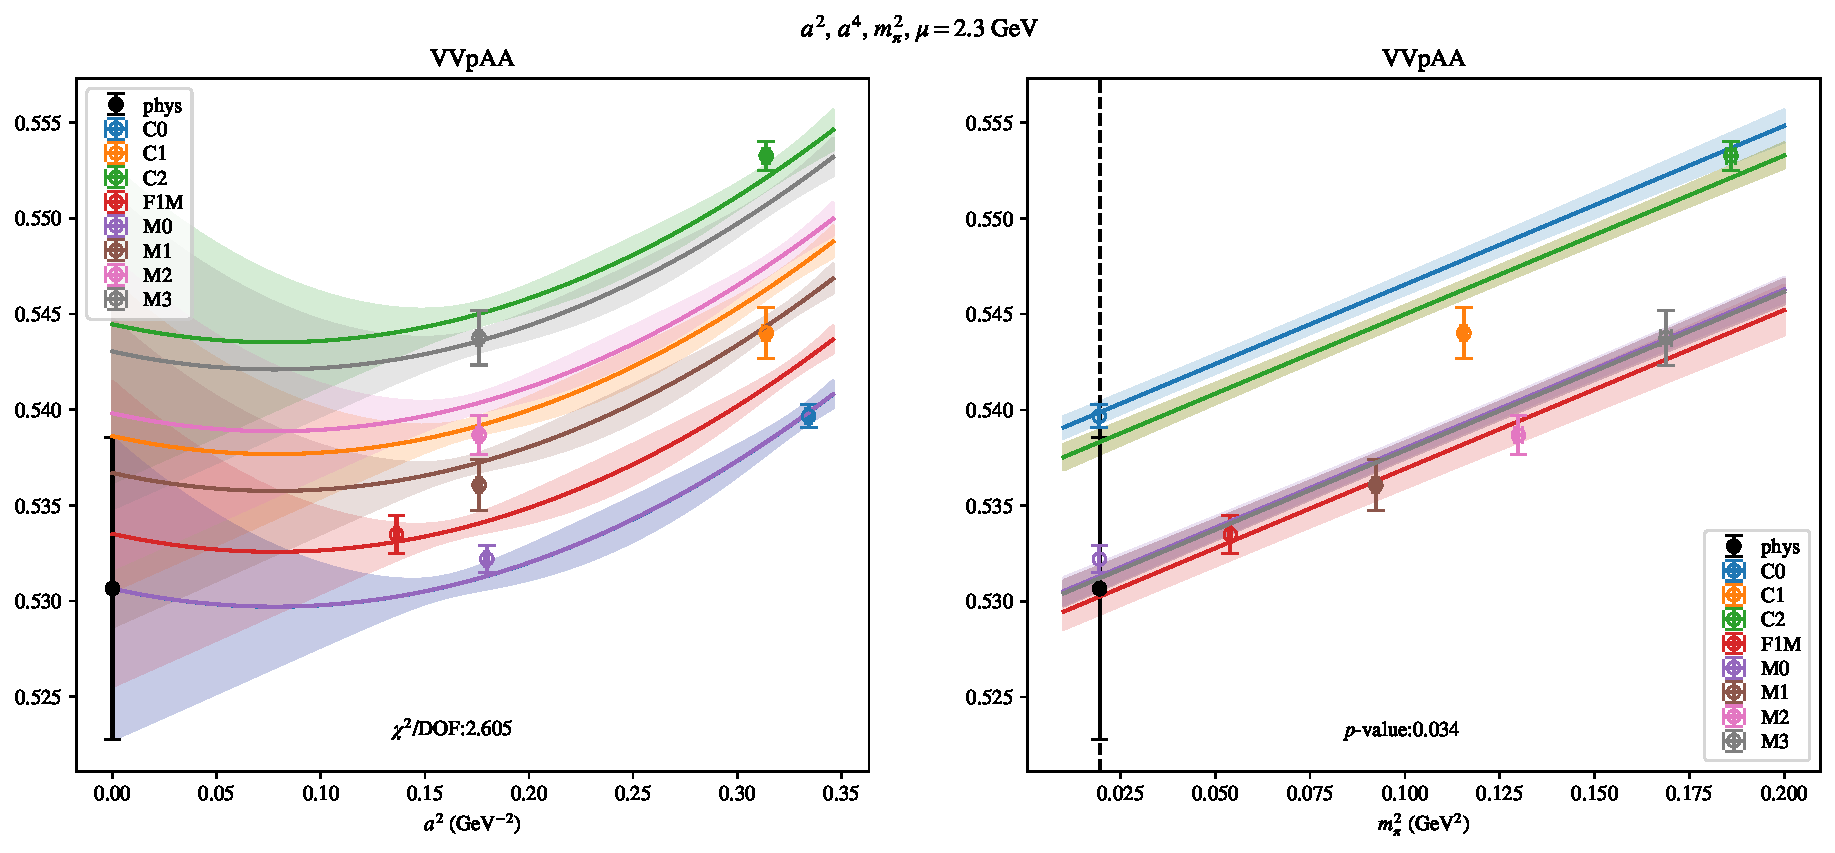
\includepdf[link, pages=-]{VVpAA/SUSY/a2a4m2_23.pdf}
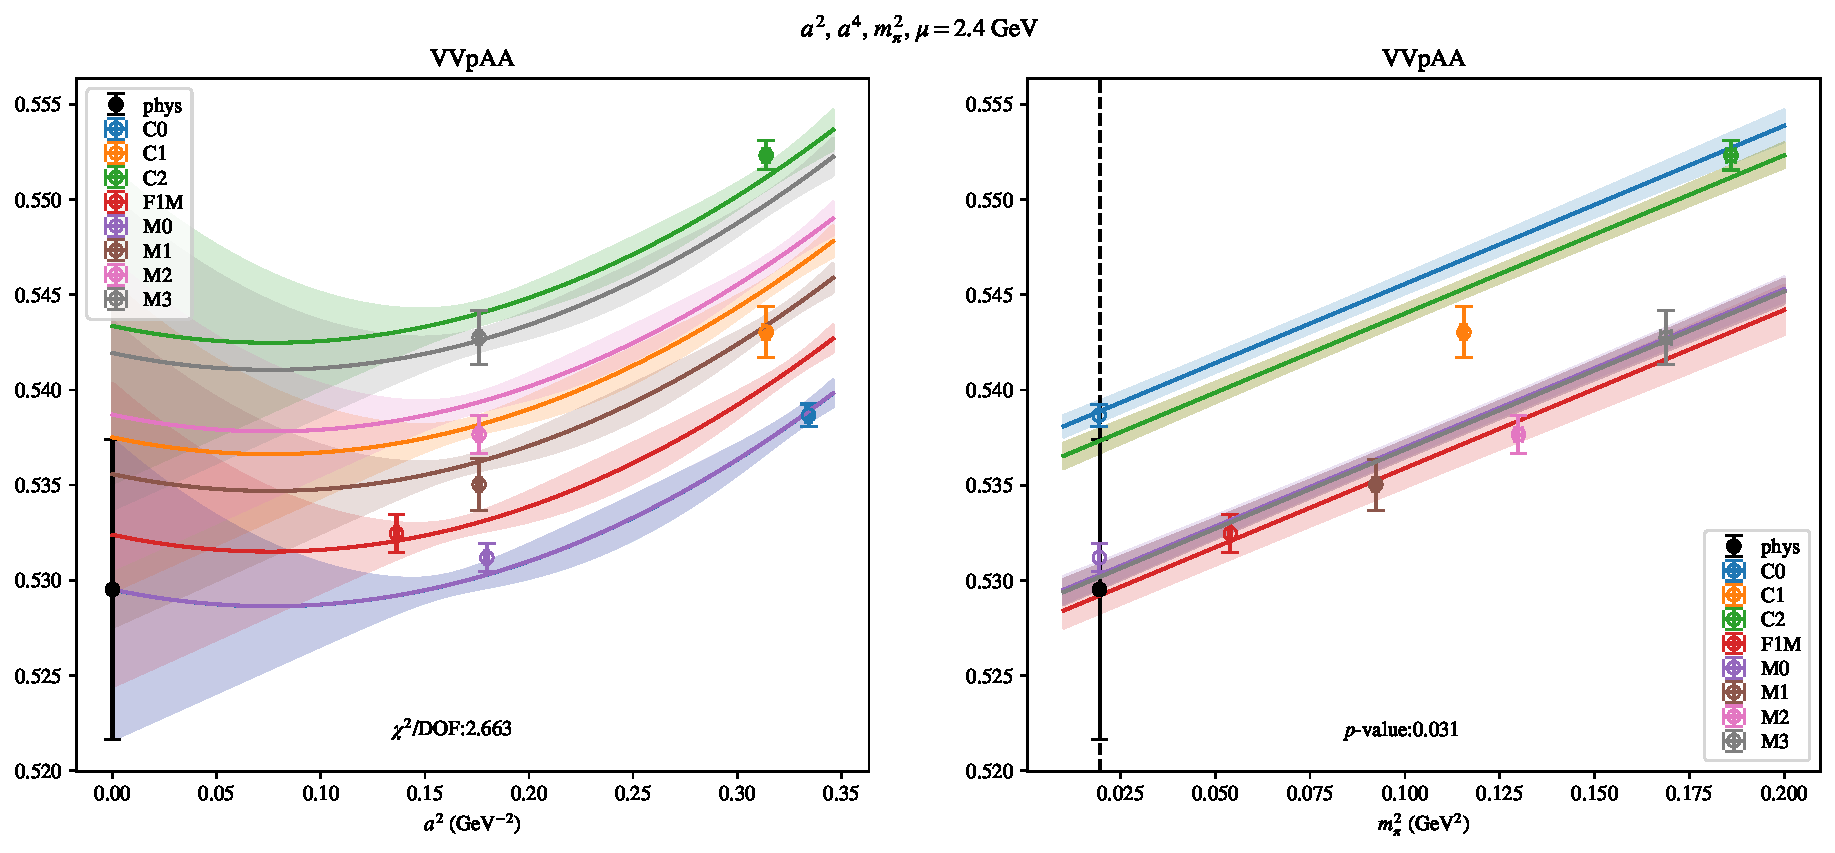
\includepdf[link, pages=-]{VVpAA/SUSY/a2a4m2_24.pdf}
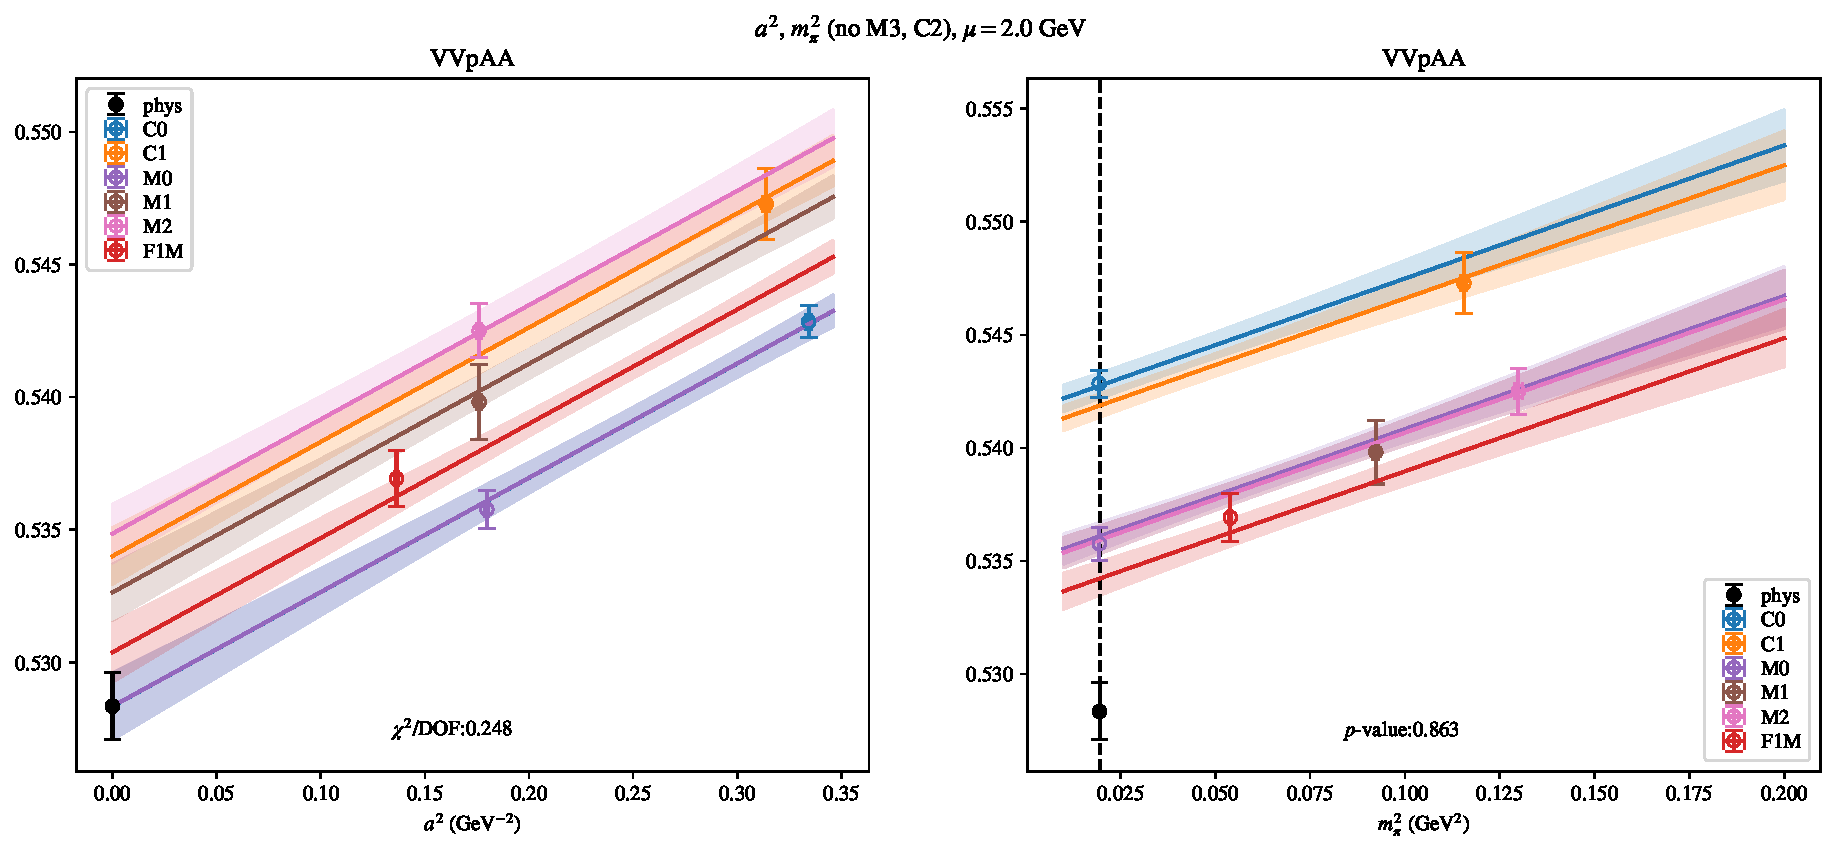
\includepdf[link, pages=-]{VVpAA/SUSY/a2m2mcut_20.pdf}
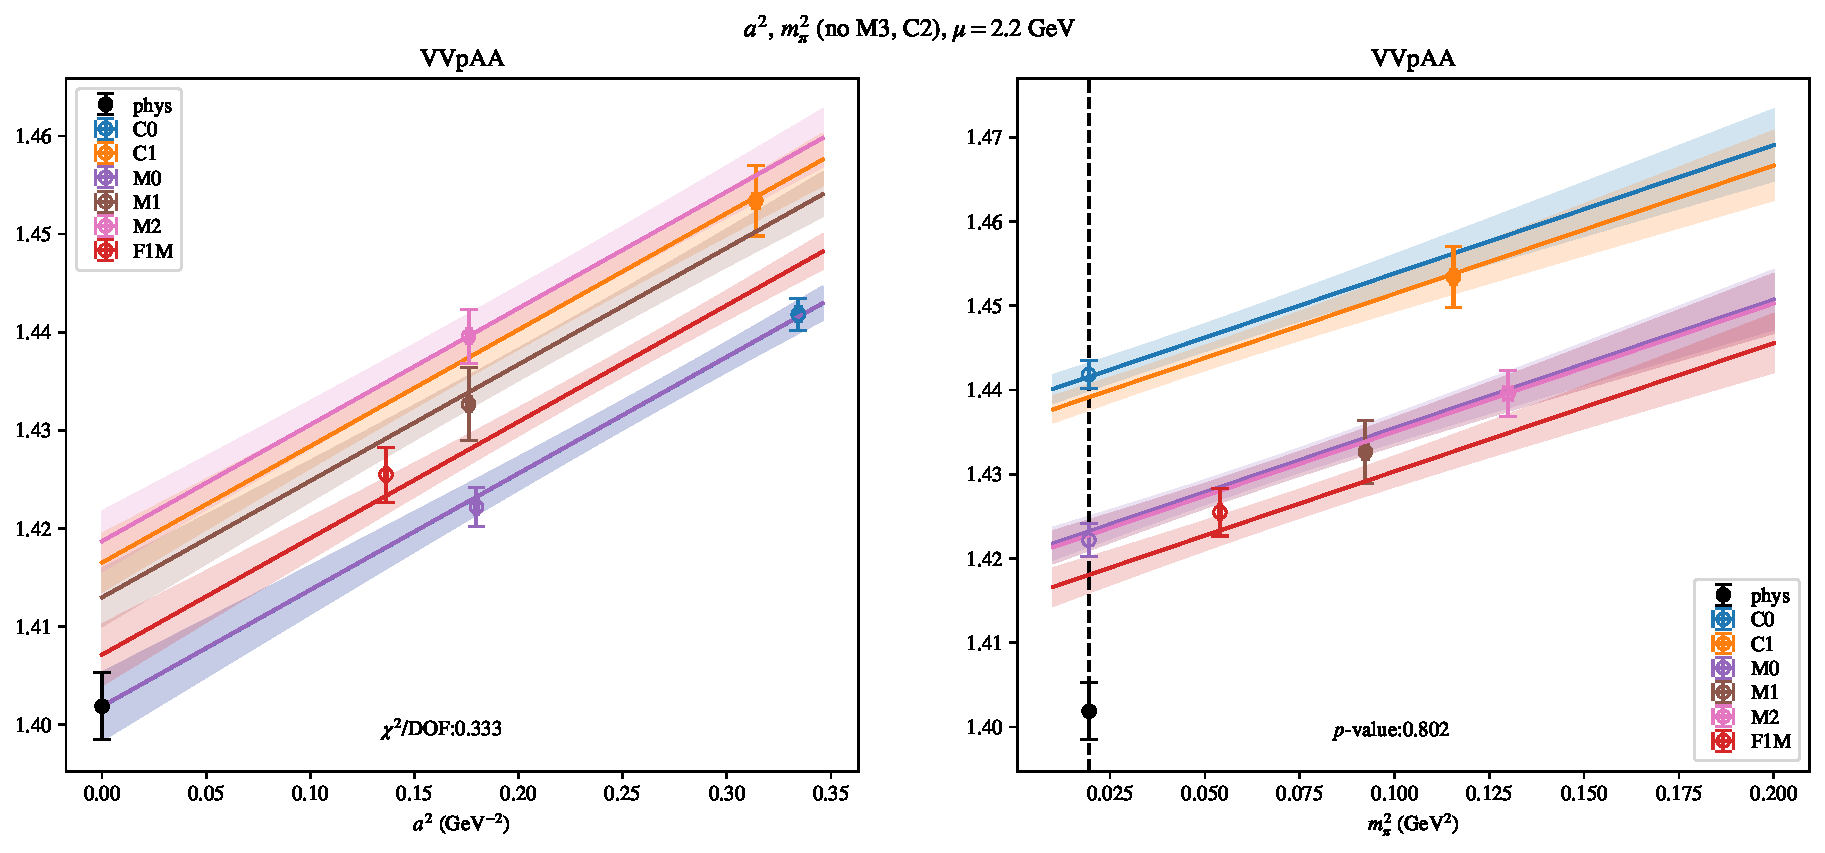
\includepdf[link, pages=-]{VVpAA/SUSY/a2m2mcut_22.pdf}
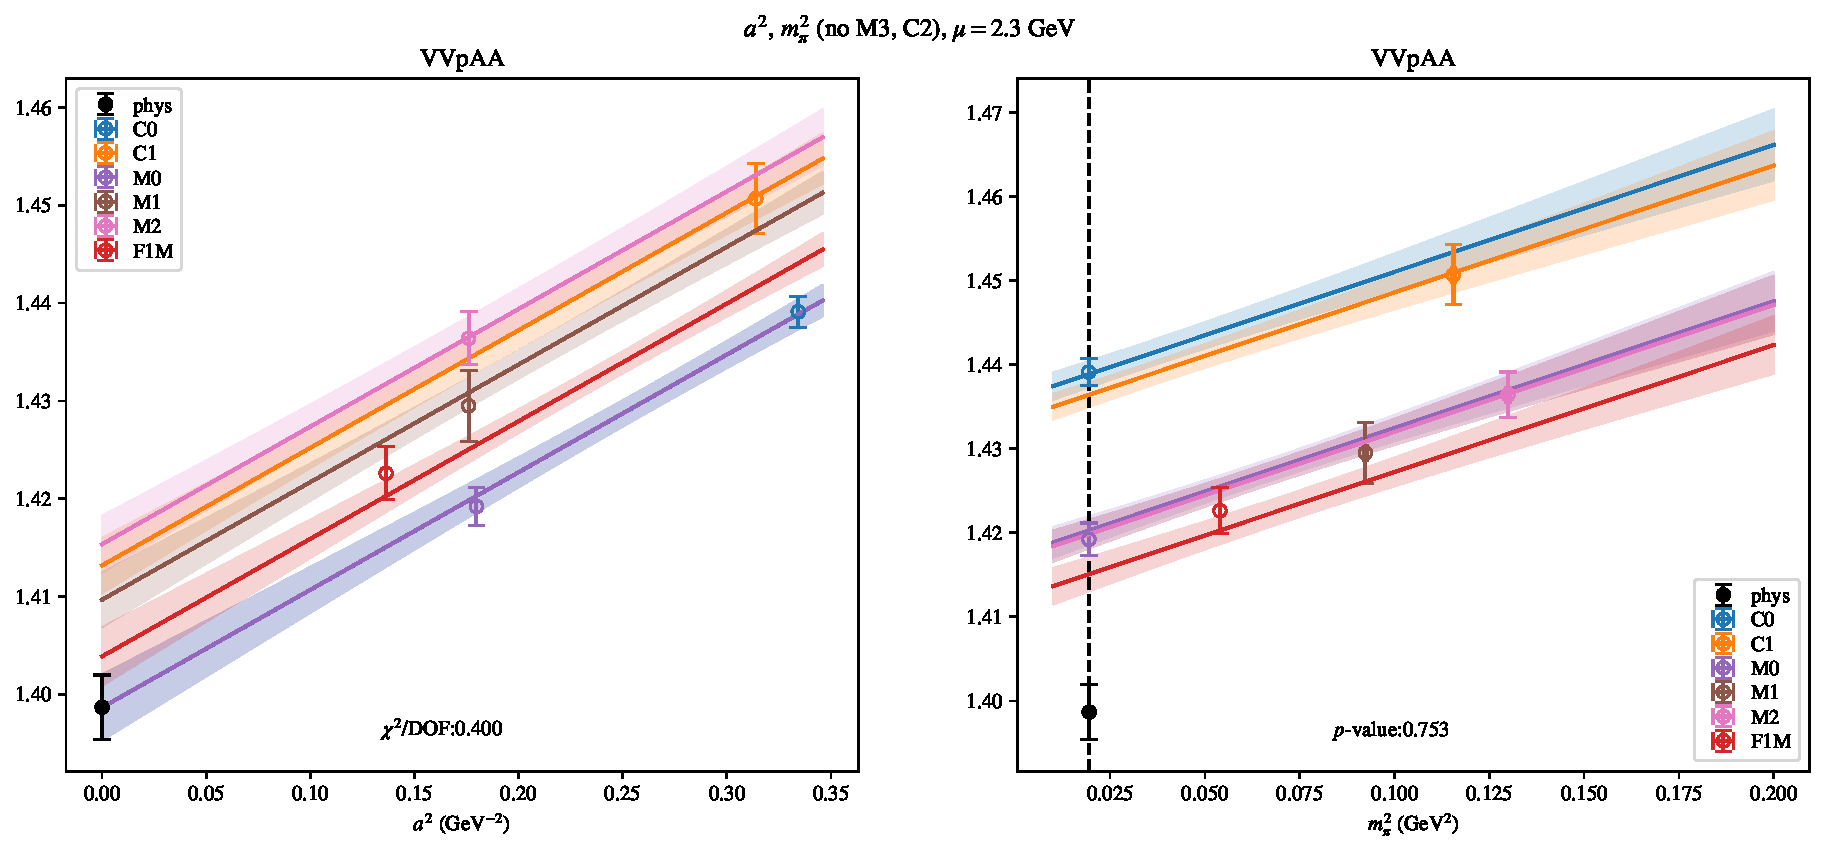
\includepdf[link, pages=-]{VVpAA/SUSY/a2m2mcut_23.pdf}
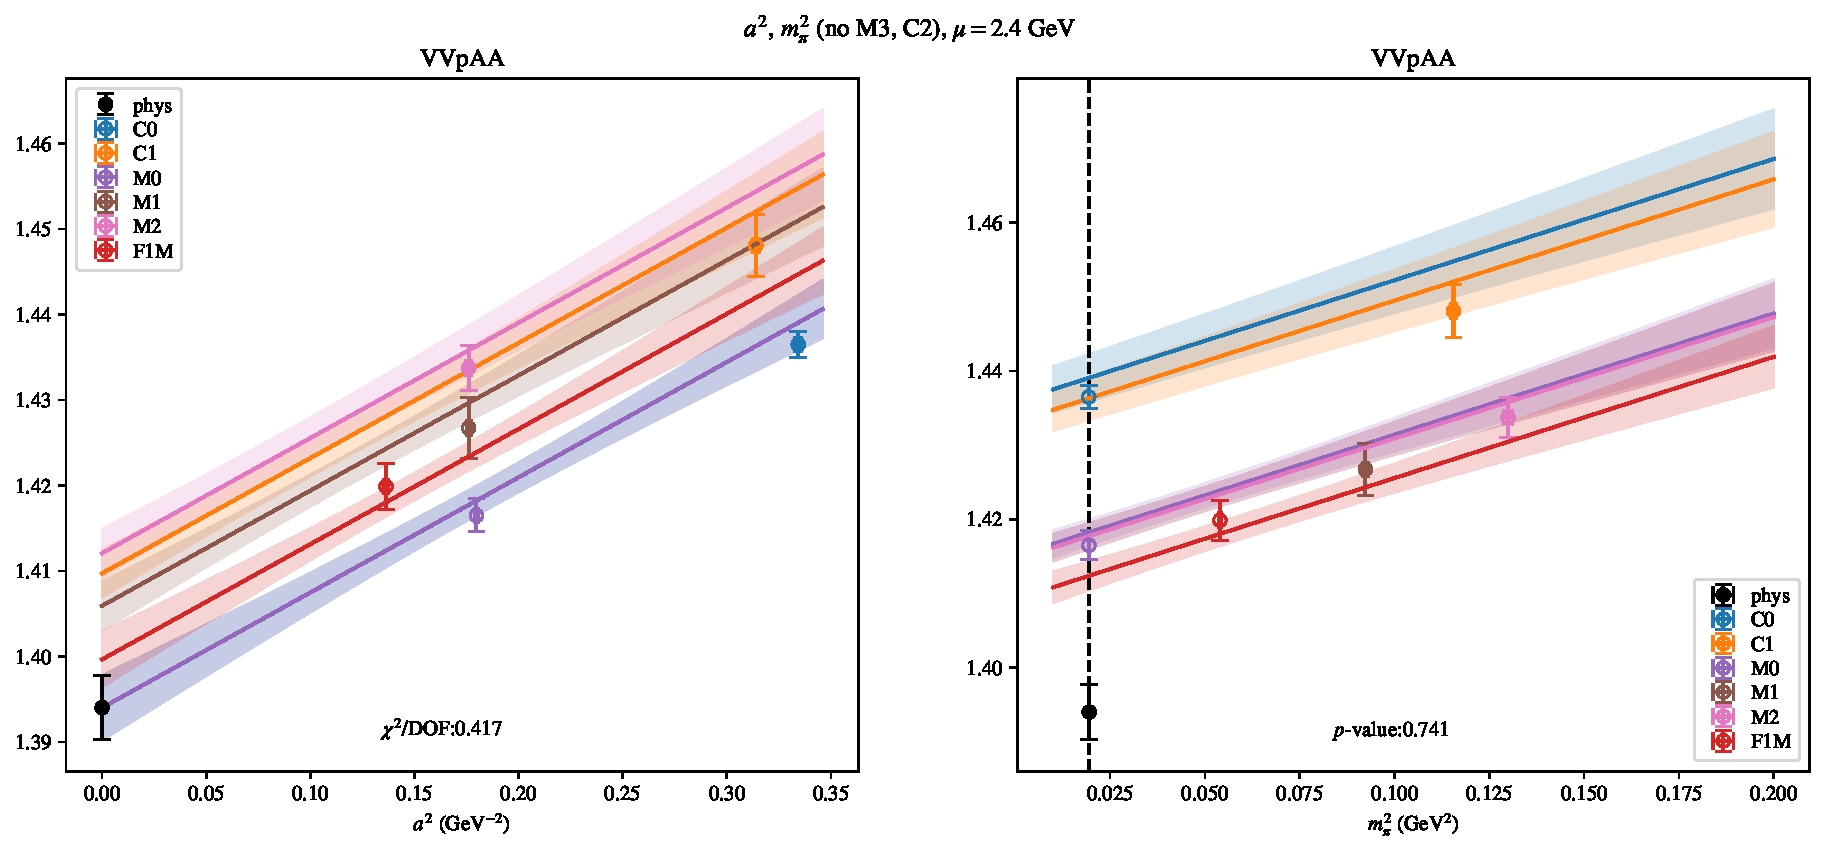
\includepdf[link, pages=-]{VVpAA/SUSY/a2m2mcut_24.pdf}
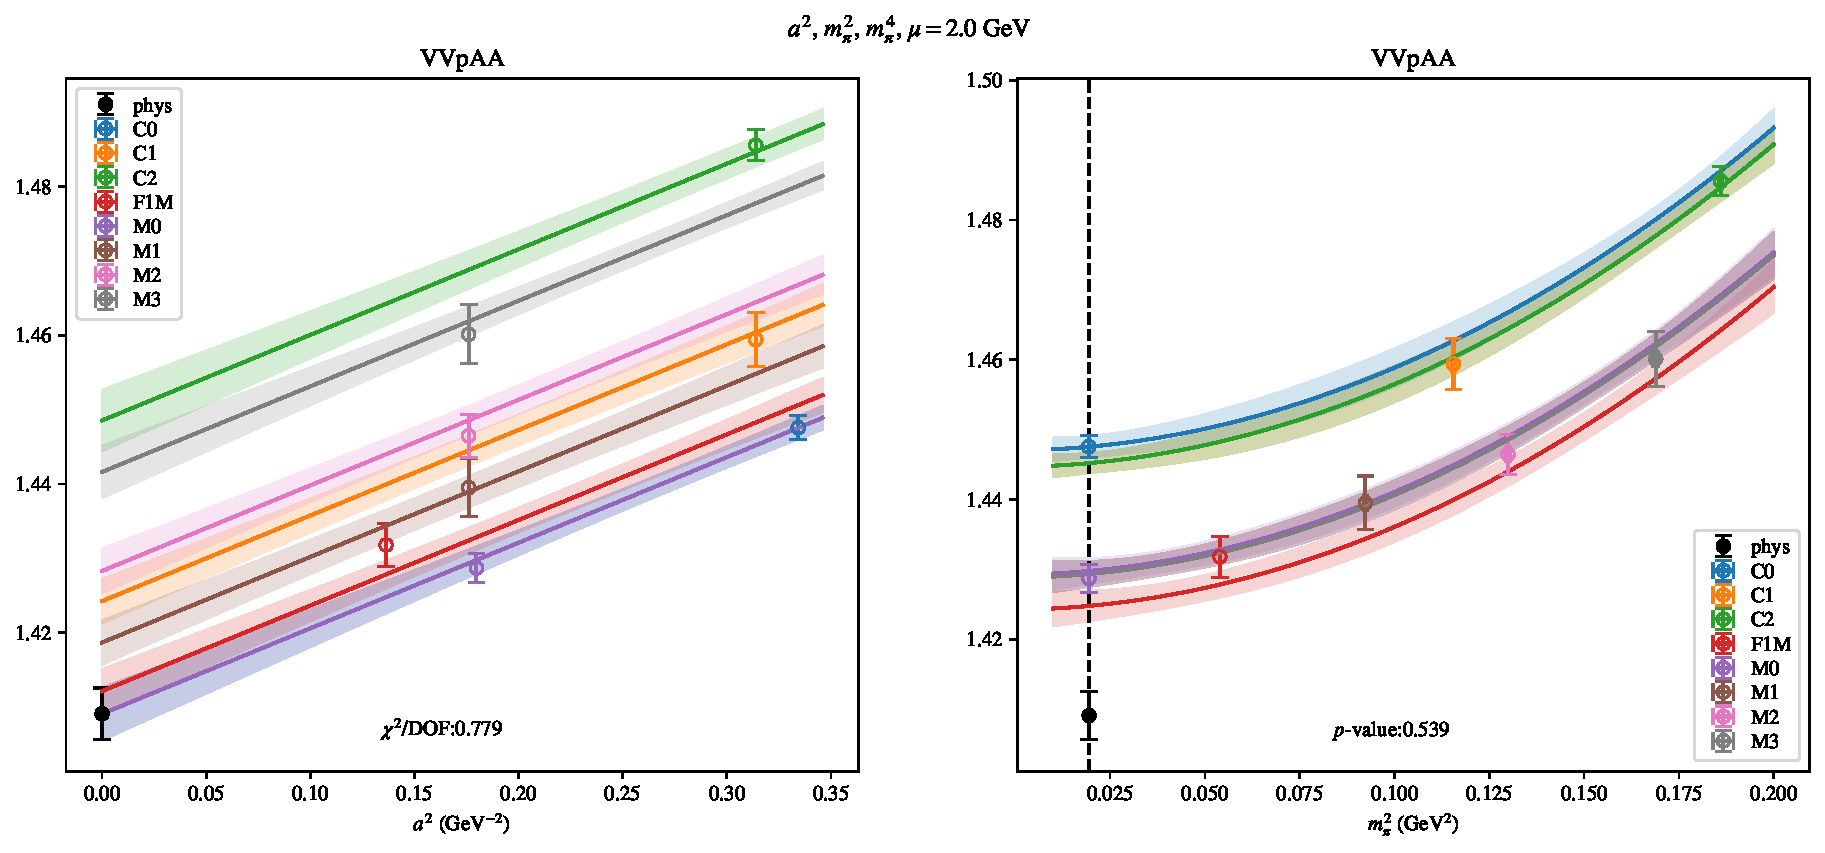
\includepdf[link, pages=-]{VVpAA/SUSY/a2m2m4_20.pdf}
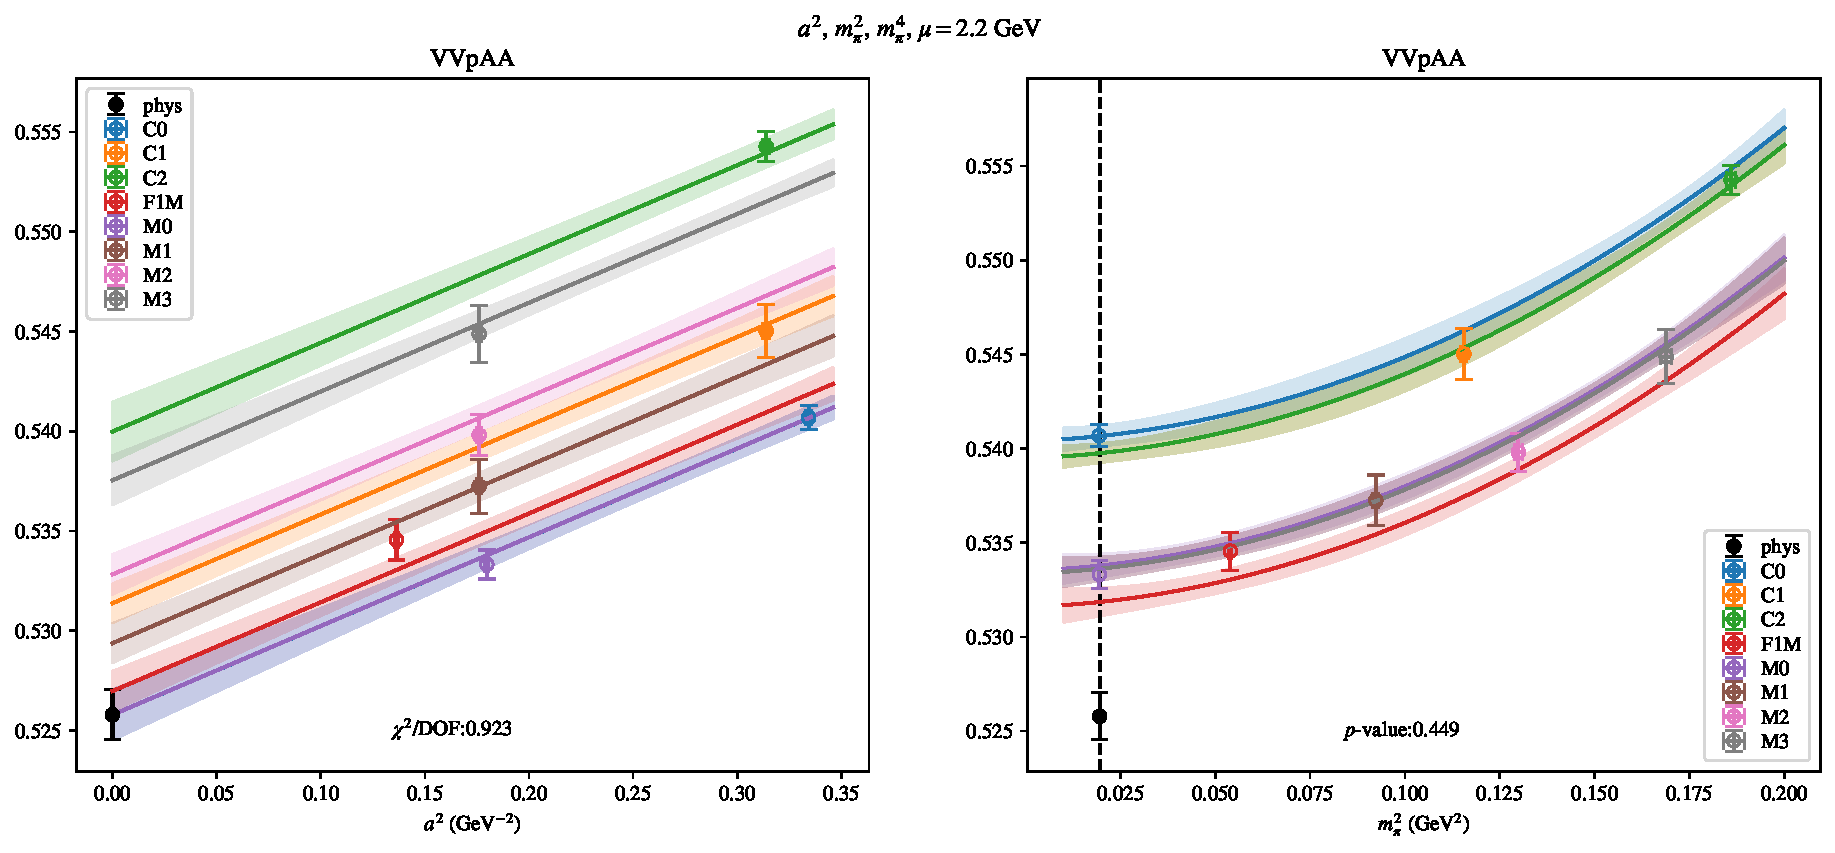
\includepdf[link, pages=-]{VVpAA/SUSY/a2m2m4_22.pdf}
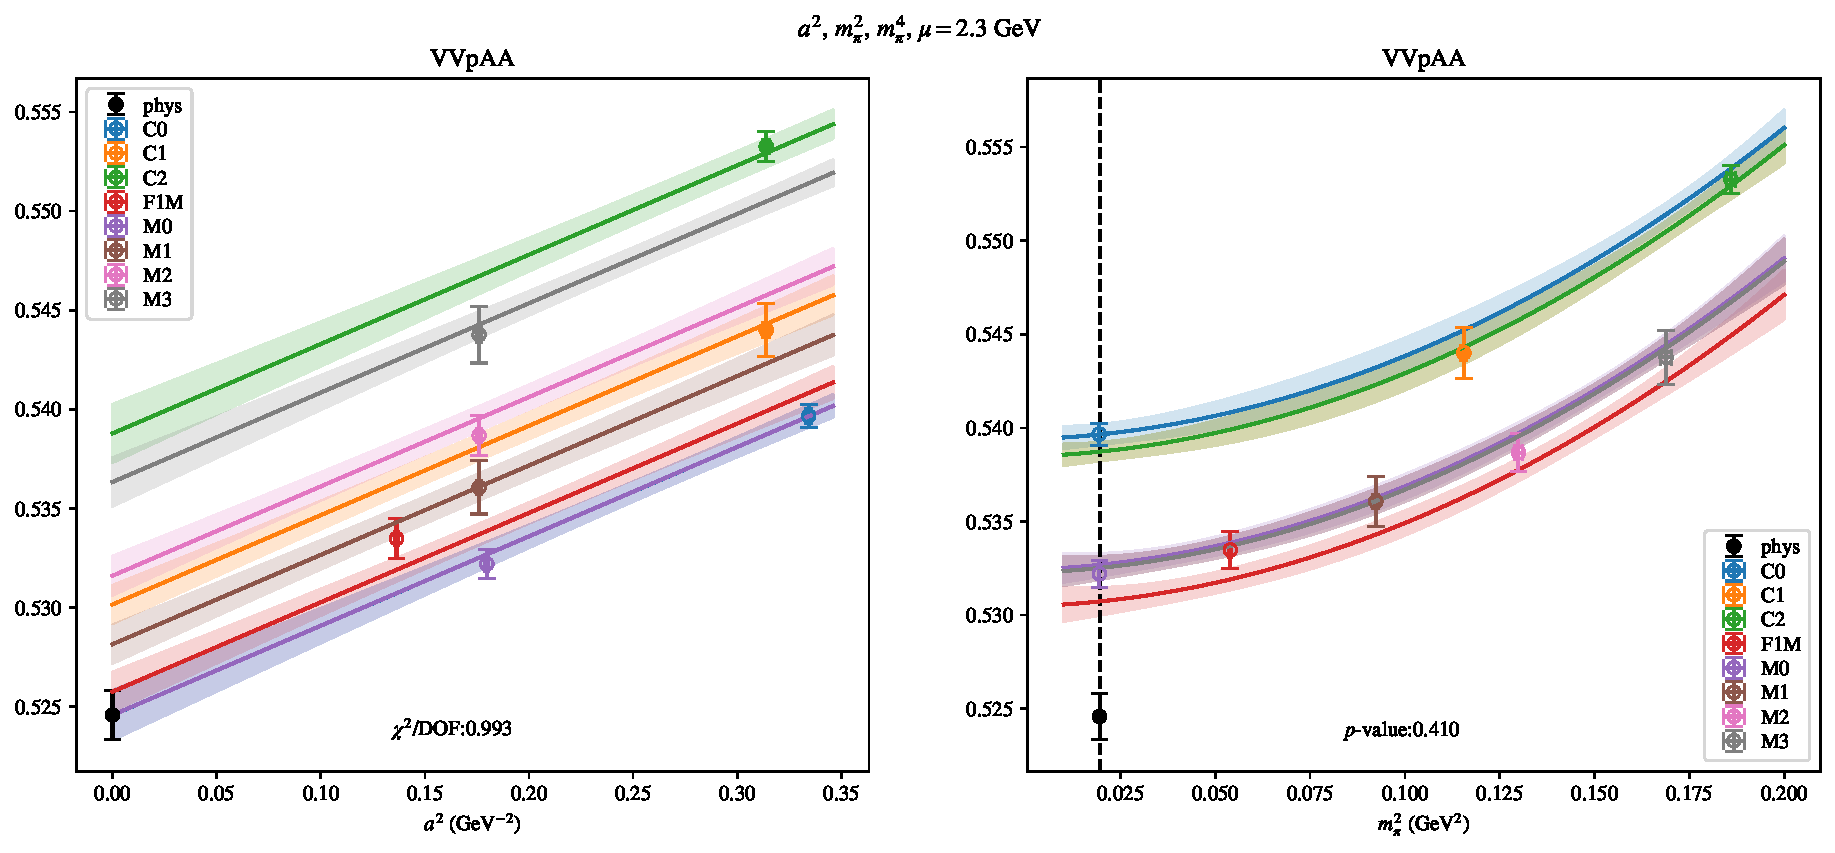
\includepdf[link, pages=-]{VVpAA/SUSY/a2m2m4_23.pdf}
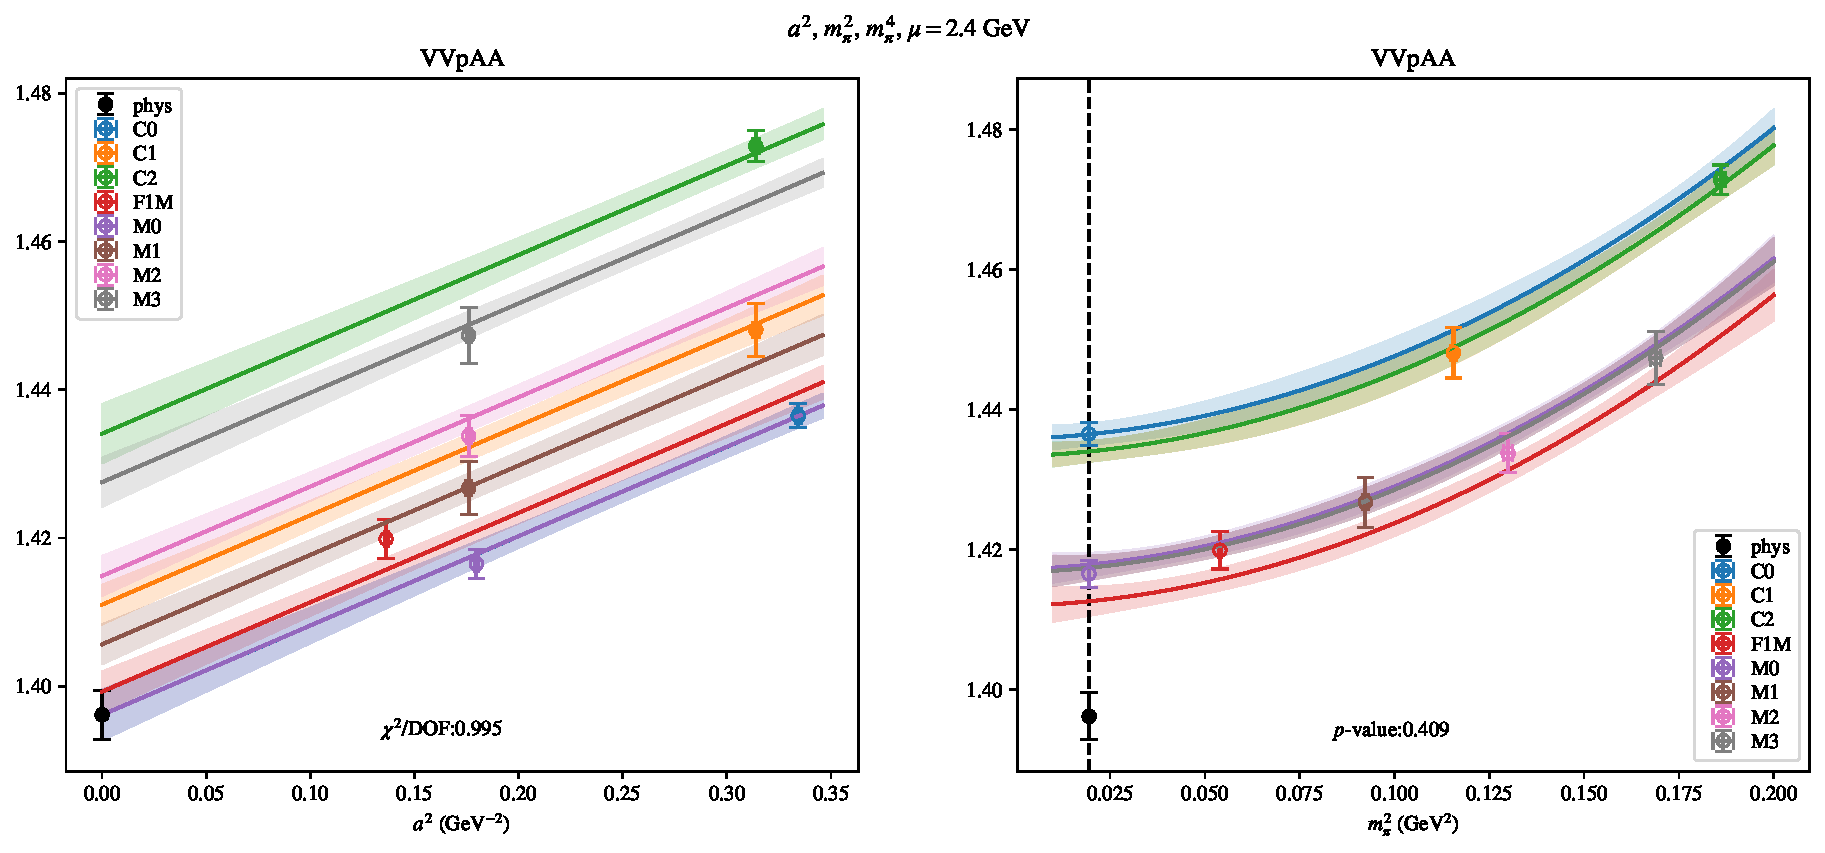
\includepdf[link, pages=-]{VVpAA/SUSY/a2m2m4_24.pdf}
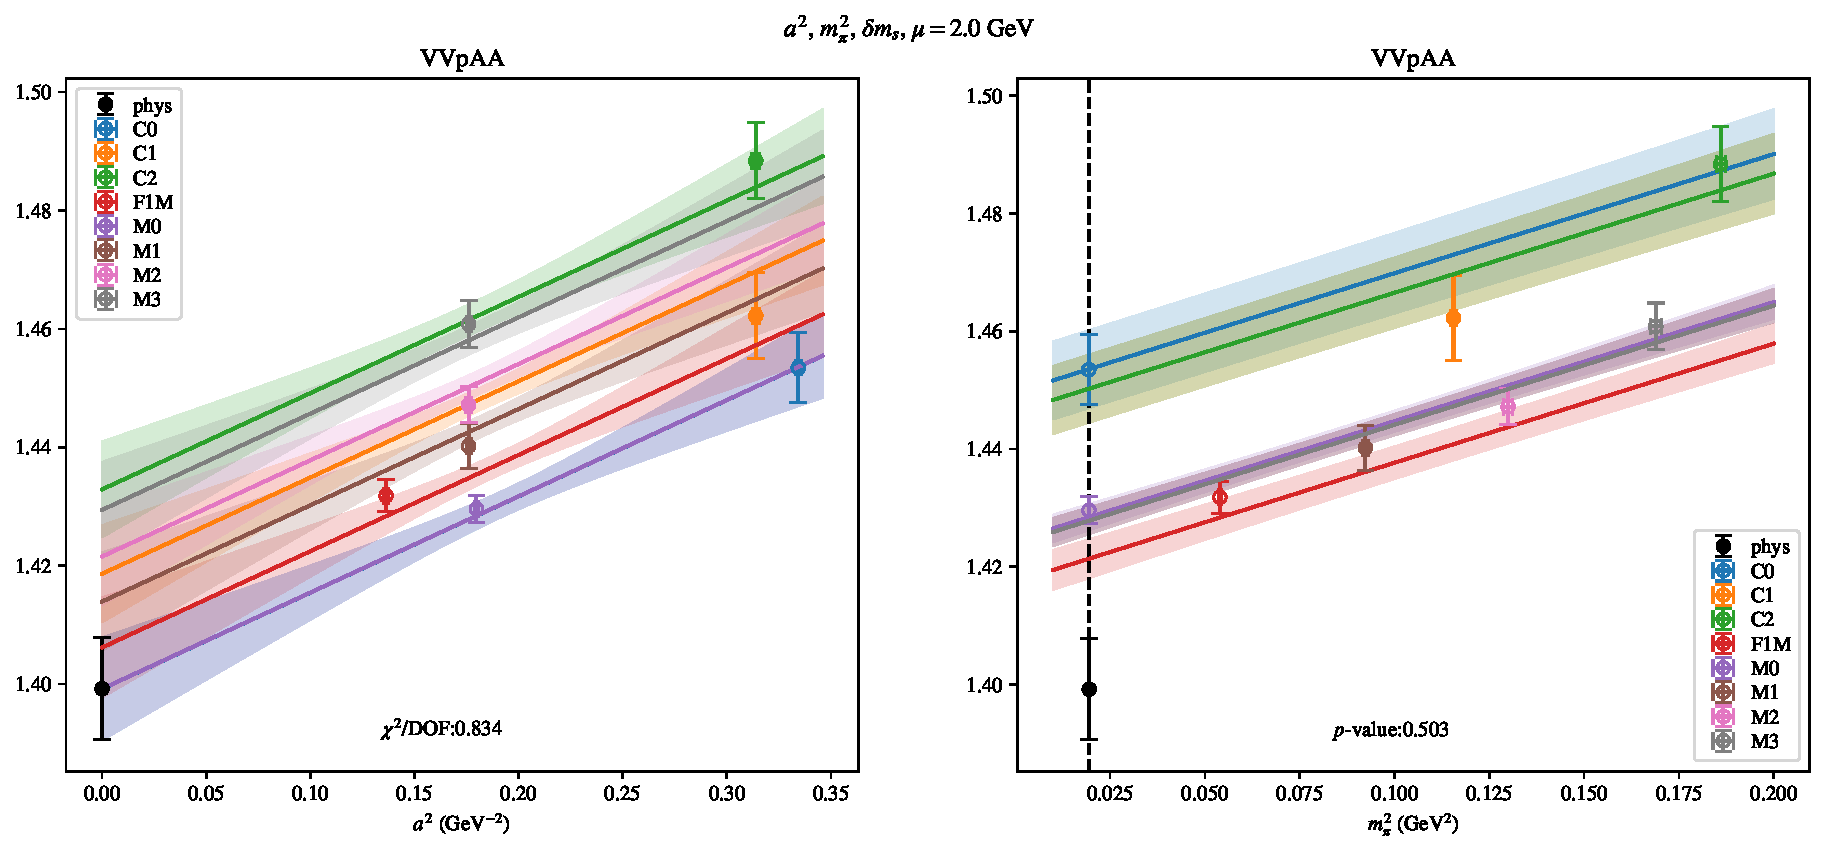
\includepdf[link, pages=-]{VVpAA/SUSY/a2m2delm_20.pdf}
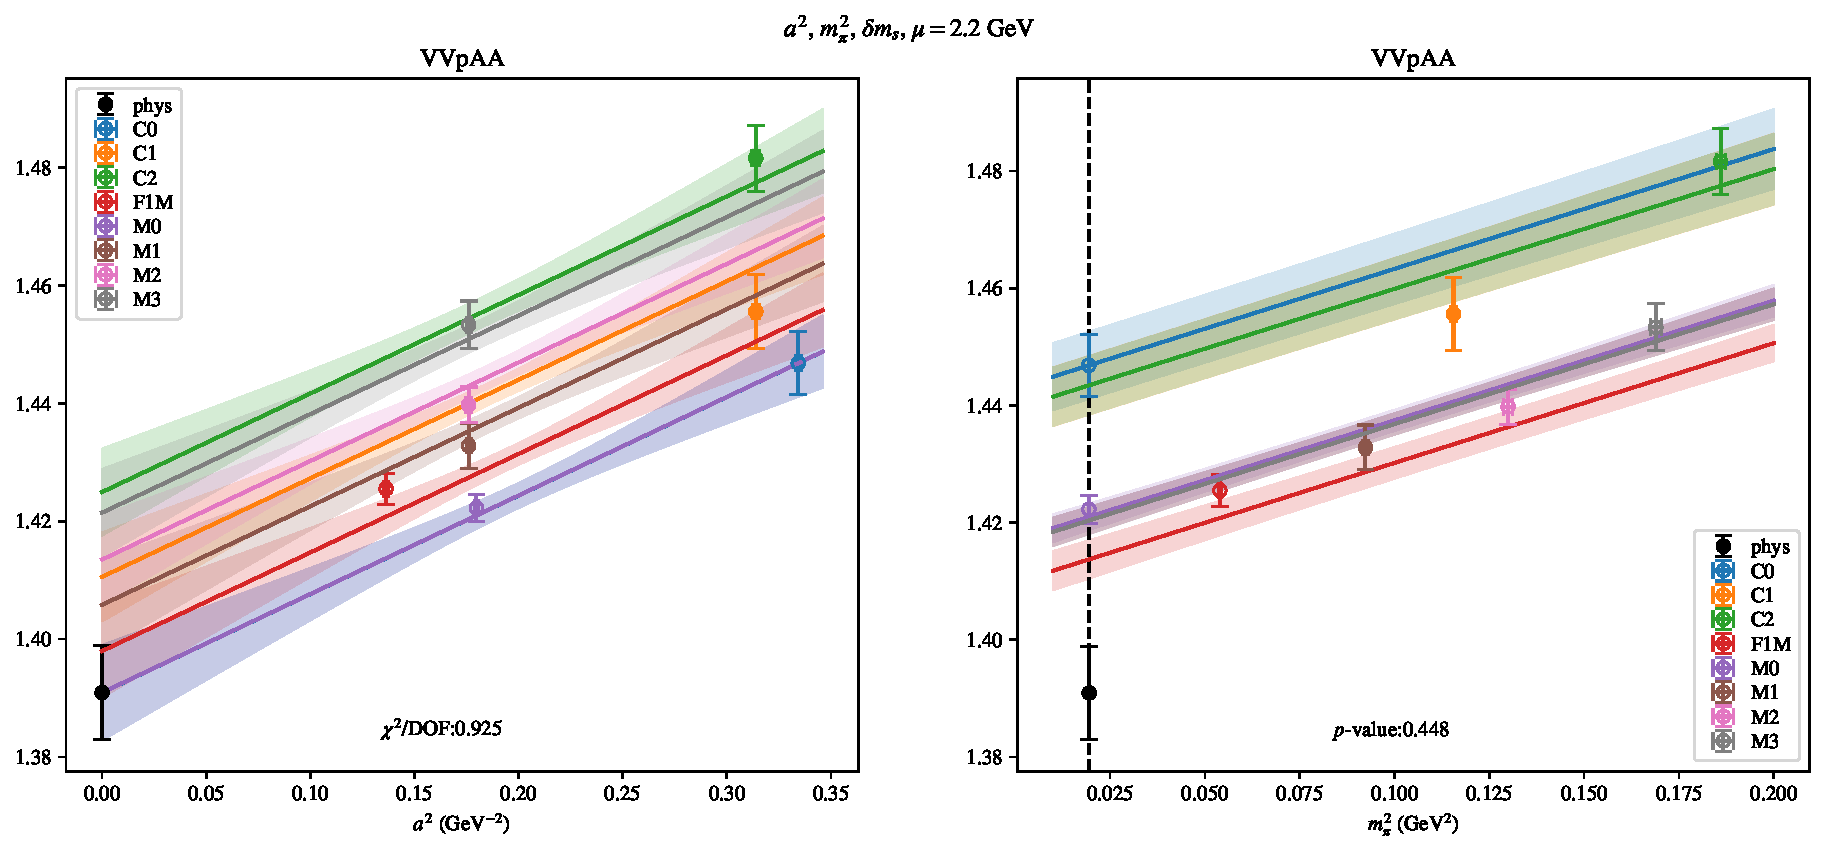
\includepdf[link, pages=-]{VVpAA/SUSY/a2m2delm_22.pdf}
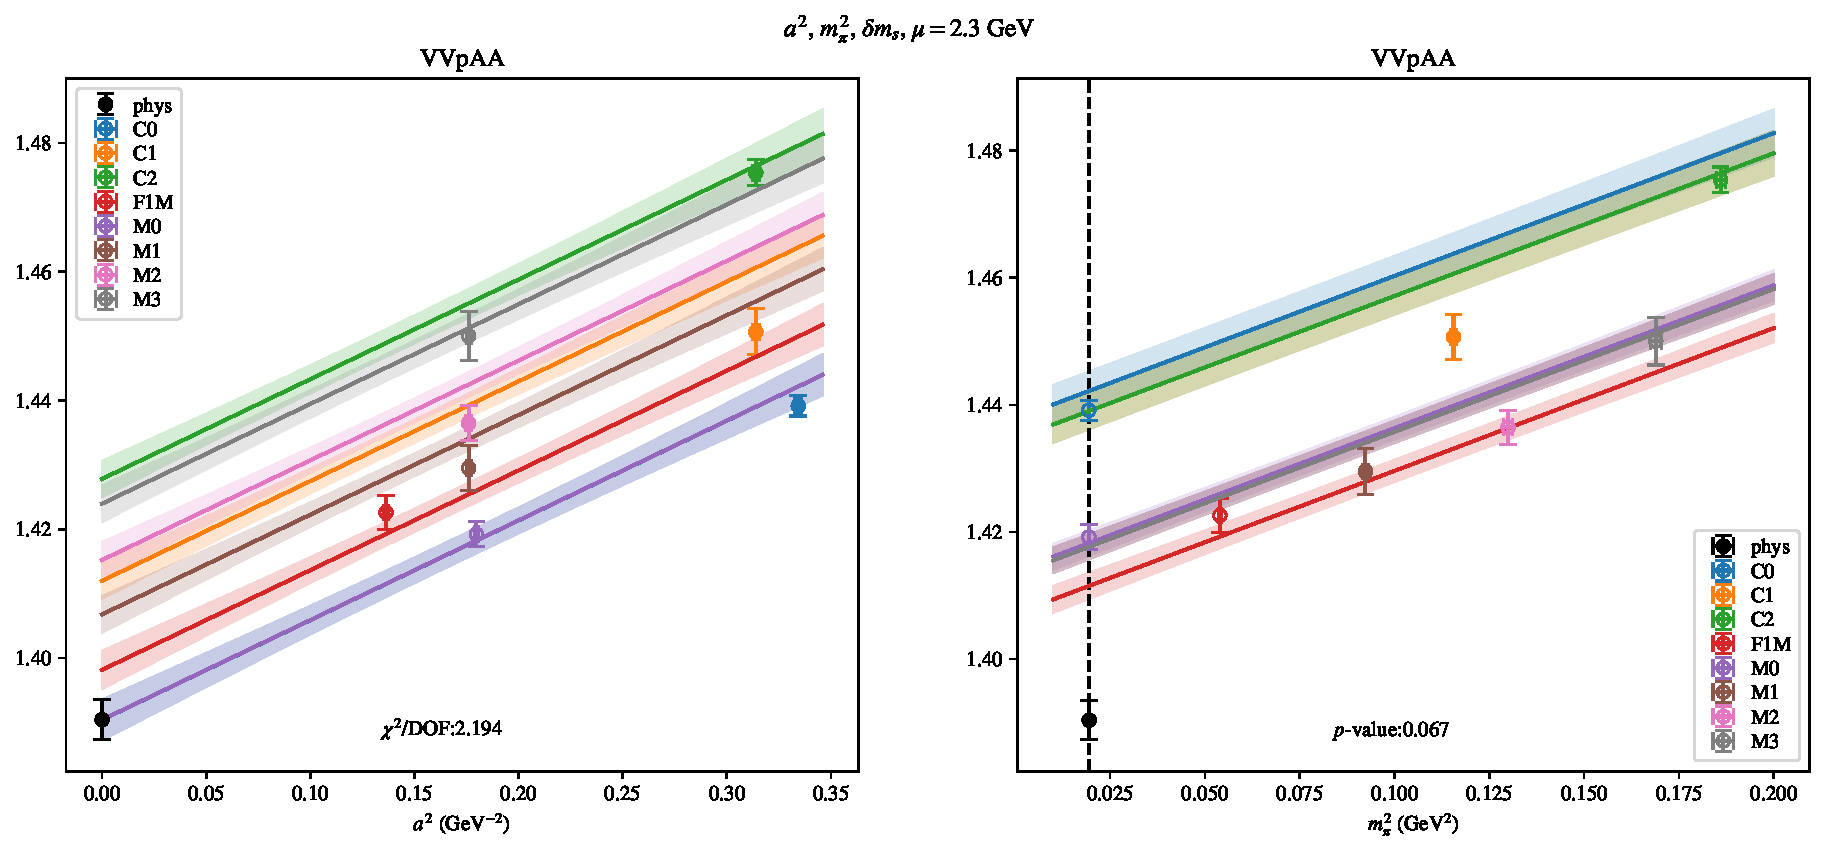
\includepdf[link, pages=-]{VVpAA/SUSY/a2m2delm_23.pdf}
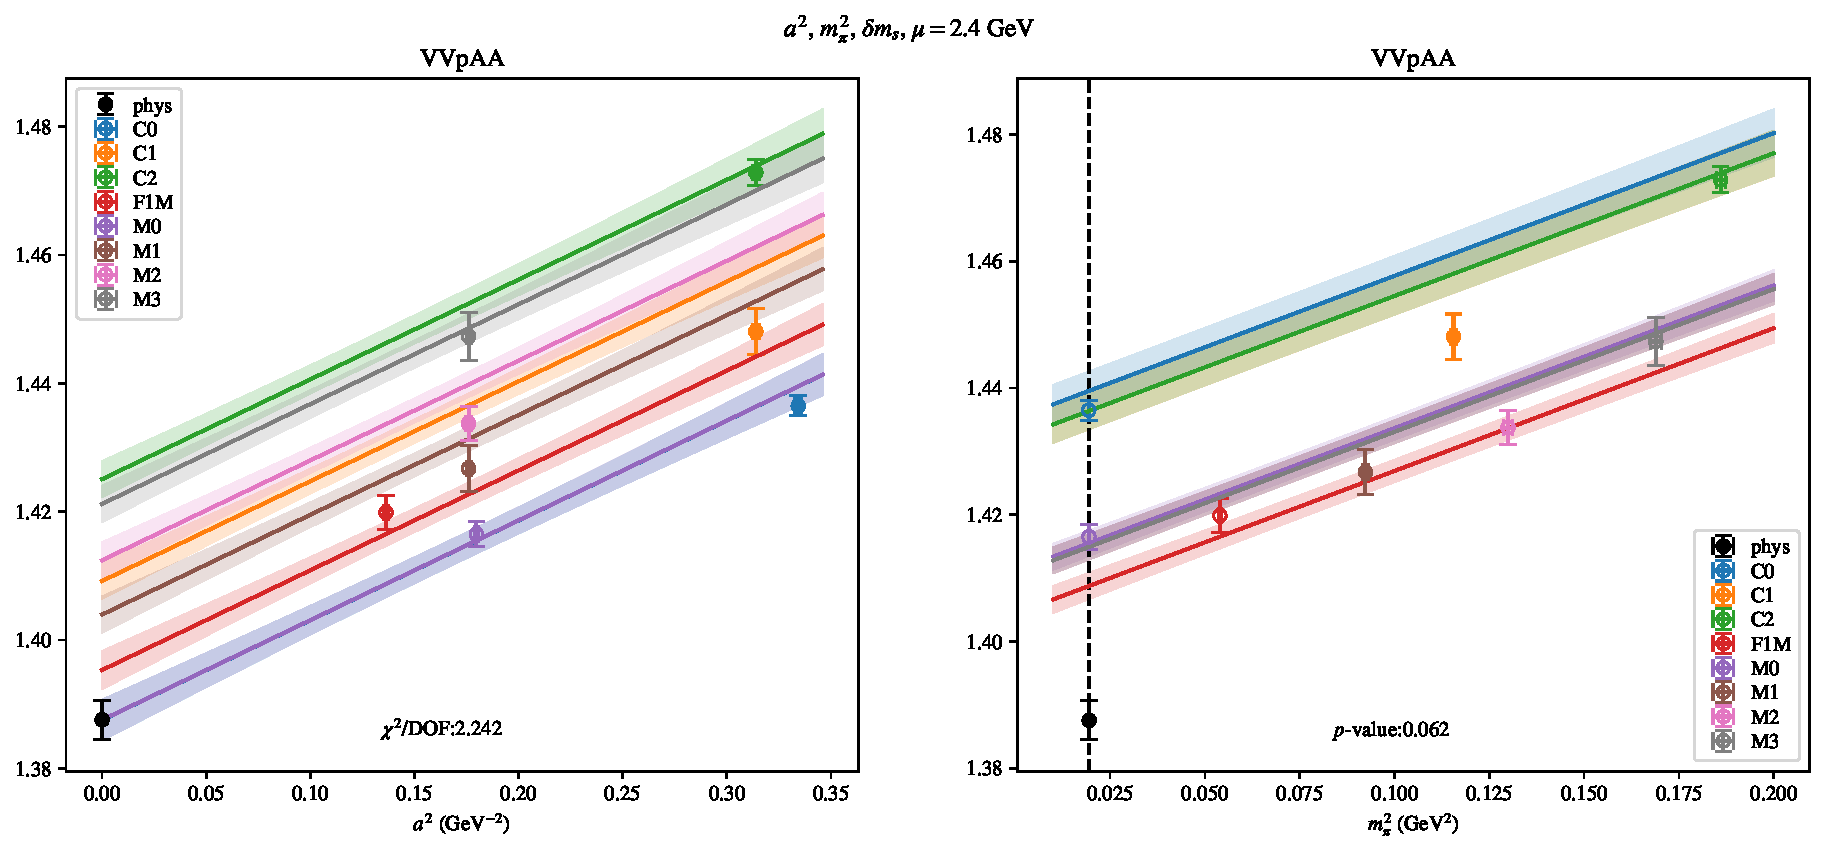
\includepdf[link, pages=-]{VVpAA/SUSY/a2m2delm_24.pdf}
\clearpage
\section{$\mathcal{B}_2$}
\begin{table}[h!]
\begin{center}
\begin{tabular}{|c|c|c|c|c|c|c|}
\hline
$\mu$ (GeV) & $a^2$, $m_\pi^2$& $a^2$, $m_\pi^2$ (no C)& $a^2$, $m_\pi^2$, $a^4$& $a^2$, $m_\pi^2$ (no M3, C2)& $a^2$, $m_\pi^2$, $m_\pi^4$& $a^2$, $m_\pi^2$, $\delta m_s$\\
\hline
2.0& \hyperlink{VVmAA/SUSY/a2m2_20.pdf.1}{\textbf{-0.924(18)}: 2.915 (0.012)} & \hyperlink{VVmAA/SUSY/a2m2noC_20.pdf.1}{\textbf{-0.933(95)}: 2.483 (0.083)} & \hyperlink{VVmAA/SUSY/a2a4m2_20.pdf.1}{\textbf{-0.91(15)}: 3.644 (0.006)} & \hyperlink{VVmAA/SUSY/a2m2mcut_20.pdf.1}{\textbf{-0.924(18)}: 3.238 (0.021)} & \hyperlink{VVmAA/SUSY/a2m2m4_20.pdf.1}{\textbf{-0.923(18)}: 2.636 (0.032)} & \hyperlink{VVmAA/SUSY/a2m2delm_20.pdf.1}{\textbf{-0.924(18)}: 3.579 (0.006)}\\
2.2& \hyperlink{VVmAA/SUSY/a2m2_22.pdf.1}{\textbf{-0.905(16)}: 3.942 (0.001)} & \hyperlink{VVmAA/SUSY/a2m2noC_22.pdf.1}{\textbf{-0.915(89)}: 2.085 (0.124)} & \hyperlink{VVmAA/SUSY/a2a4m2_22.pdf.1}{\textbf{-0.90(15)}: 4.927 (0.001)} & \hyperlink{VVmAA/SUSY/a2m2mcut_22.pdf.1}{\textbf{-0.905(18)}: 4.252 (0.005)} & \hyperlink{VVmAA/SUSY/a2m2m4_22.pdf.1}{\textbf{-0.905(19)}: 4.16 (0.002)} & \hyperlink{VVmAA/SUSY/a2m2delm_22.pdf.1}{\textbf{-0.905(16)}: 4.687 (0.001)}\\
2.3& \hyperlink{VVmAA/SUSY/a2m2_23.pdf.1}{\textbf{-0.896(15)}: 4.412 (0.001)} & \hyperlink{VVmAA/SUSY/a2m2noC_23.pdf.1}{\textbf{-0.908(87)}: 2.403 (0.09)} & \hyperlink{VVmAA/SUSY/a2a4m2_23.pdf.1}{\textbf{-0.90(15)}: 5.507 (0.0)} & \hyperlink{VVmAA/SUSY/a2m2mcut_23.pdf.1}{\textbf{-0.896(18)}: 4.95 (0.002)} & \hyperlink{VVmAA/SUSY/a2m2m4_23.pdf.1}{\textbf{-0.896(18)}: 4.577 (0.001)} & \hyperlink{VVmAA/SUSY/a2m2delm_23.pdf.1}{\textbf{-0.896(16)}: 5.175 (0.0)}\\
2.4& \hyperlink{VVmAA/SUSY/a2m2_24.pdf.1}{\textbf{-0.889(15)}: 4.813 (0.0)} & \hyperlink{VVmAA/SUSY/a2m2noC_24.pdf.1}{\textbf{-0.901(86)}: 2.54 (0.079)} & \hyperlink{VVmAA/SUSY/a2a4m2_24.pdf.1}{\textbf{-0.89(15)}: 6.011 (0.0)} & \hyperlink{VVmAA/SUSY/a2m2mcut_24.pdf.1}{\textbf{-0.888(18)}: 5.54 (0.001)} & \hyperlink{VVmAA/SUSY/a2m2m4_24.pdf.1}{\textbf{-0.888(18)}: 5.111 (0.0)} & \hyperlink{VVmAA/SUSY/a2m2delm_24.pdf.1}{\textbf{-0.888(15)}: 5.654 (0.0)}\\
\hline
\end{tabular}
\caption{Physical point value from chiral and continuum extrapolation at renormalisation scale $\mu$. Entries are \textbf{value(error)}: $\chi^2/\text{DOF}$ ($p$-value).}
\end{center}
\end{table}
\begin{table}[h!]
\begin{center}
\begin{tabular}{|c c|c|c|c|c|c|c|}
\hline
$\mu$ (GeV) &  & $a^2$, $m_\pi^2$& $a^2$, $m_\pi^2$ (no C)& $a^2$, $m_\pi^2$, $a^4$& $a^2$, $m_\pi^2$ (no M3, C2)& $a^2$, $m_\pi^2$, $m_\pi^4$& $a^2$, $m_\pi^2$, $\delta m_s$\\
\hline
\multirow{3}{0.5in}{2.0} & $\alpha$ & 0.3834(94)& 0.330(62)& 0.43(16)& 0.3822(90)& 0.3868(89)& 0.3841(98)\\
 & $\beta$ & 0.00638(25)& 0.00580(44)& 0.00639(26)& 0.00660(43)& 0.0073(11)& 0.00640(25)\\
 & $\gamma$ &  &  & -0.099&  & -8.62265(93)& -0.001\\
\hline
\multirow{3}{0.5in}{2.2} & $\alpha$ & 0.4268(76)& 0.365(59)& 0.42(16)& 0.4273(94)& 0.4290(81)& 0.4282(79)\\
 & $\beta$ & 0.00683(21)& 0.00643(25)& 0.00683(23)& 0.00694(42)& 0.0074(11)& 0.00688(21)\\
 & $\gamma$ &  &  & 0.013&  & -5.24380(90)& -0.001(24)\\
\hline
\multirow{3}{0.5in}{2.3} & $\alpha$ & 0.4490(77)& 0.372(58)& 0.40(16)& 0.4500(97)& 0.4515(81)& 0.4507(80)\\
 & $\beta$ & 0.00693(20)& 0.00653(24)& 0.00692(23)& 0.00704(42)& 0.0075(11)& 0.00700(20)\\
 & $\gamma$ &  &  & 0.077&  & -5.80572(93)& -0.002(24)\\
\hline
\multirow{3}{0.5in}{2.4} & $\alpha$ & 0.4683(76)& 0.386(59)& 0.42(16)& 0.4690(98)& 0.4708(81)& 0.4701(80)\\
 & $\beta$ & 0.00703(20)& 0.00659(23)& 0.00701(23)& 0.00714(38)& 0.0077(11)& 0.00710(20)\\
 & $\gamma$ &  &  & 0.077&  & -5.89874(90)& -0.002(24)\\
\hline
\end{tabular}
\caption{Fit values of coefficients in $Q = Q_{phys} + \mathbf{\alpha} a^2 + \mathbf{\beta}\left(\frac{m_\pi^2}{f_\pi^2}-\frac{m_{\pi,PDG}^2}{f_\pi^2}\right) + \gamma(\ldots)$}
\end{center}
\end{table}
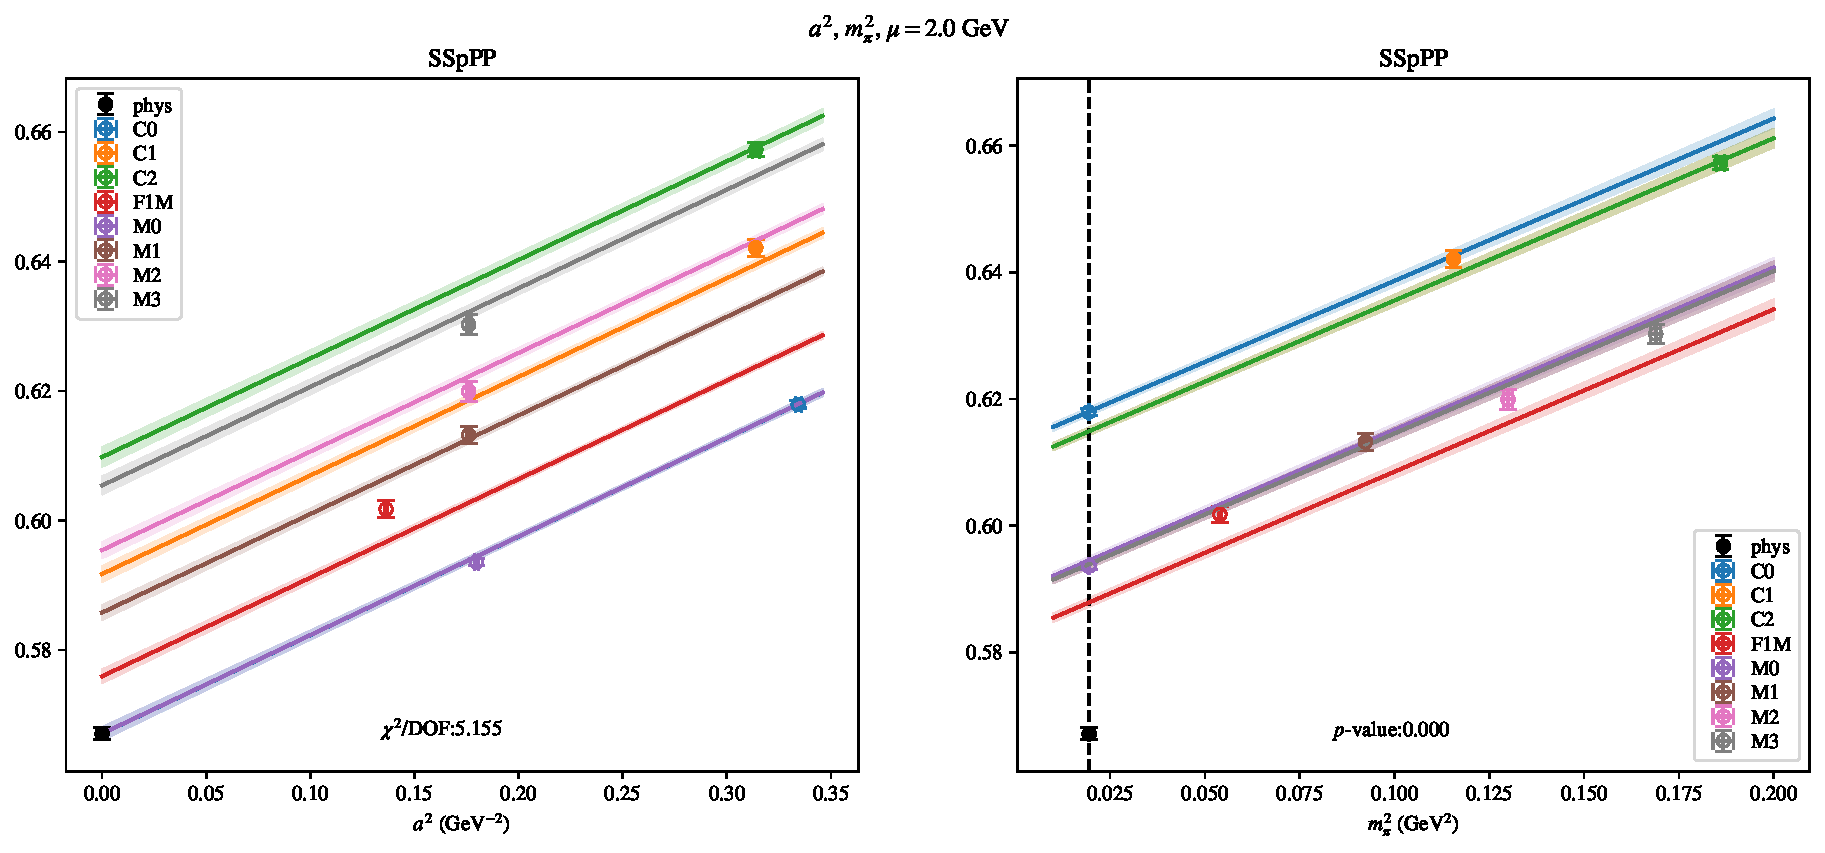
\includepdf[link, pages=-]{VVmAA/SUSY/a2m2_20.pdf}
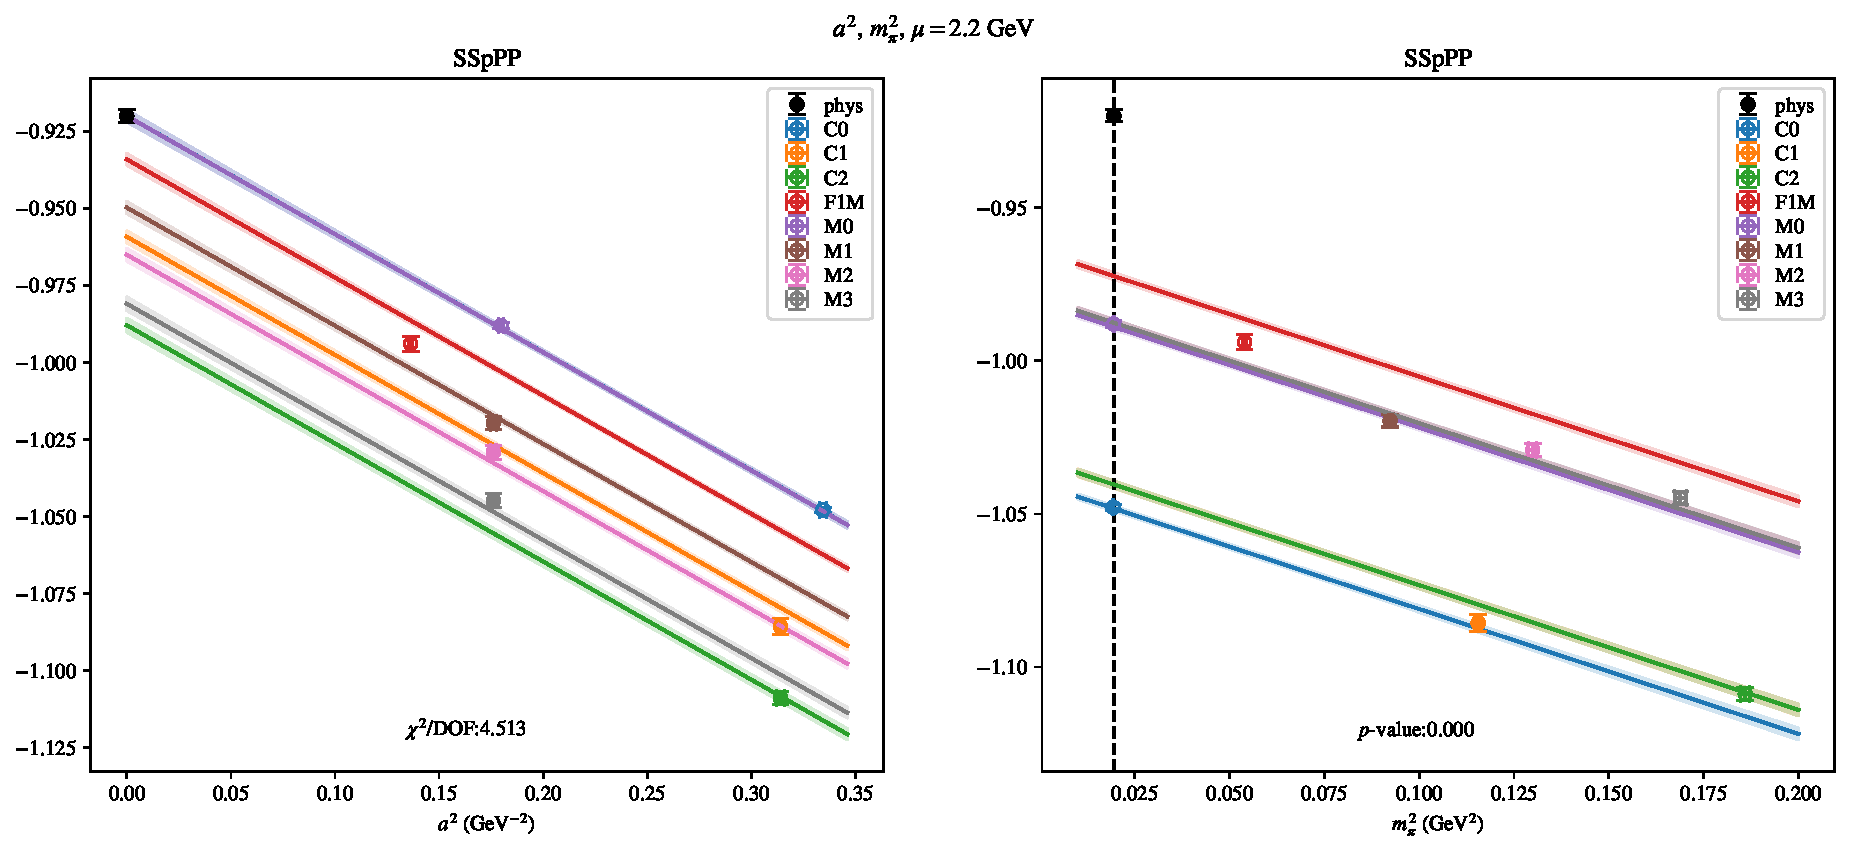
\includepdf[link, pages=-]{VVmAA/SUSY/a2m2_22.pdf}
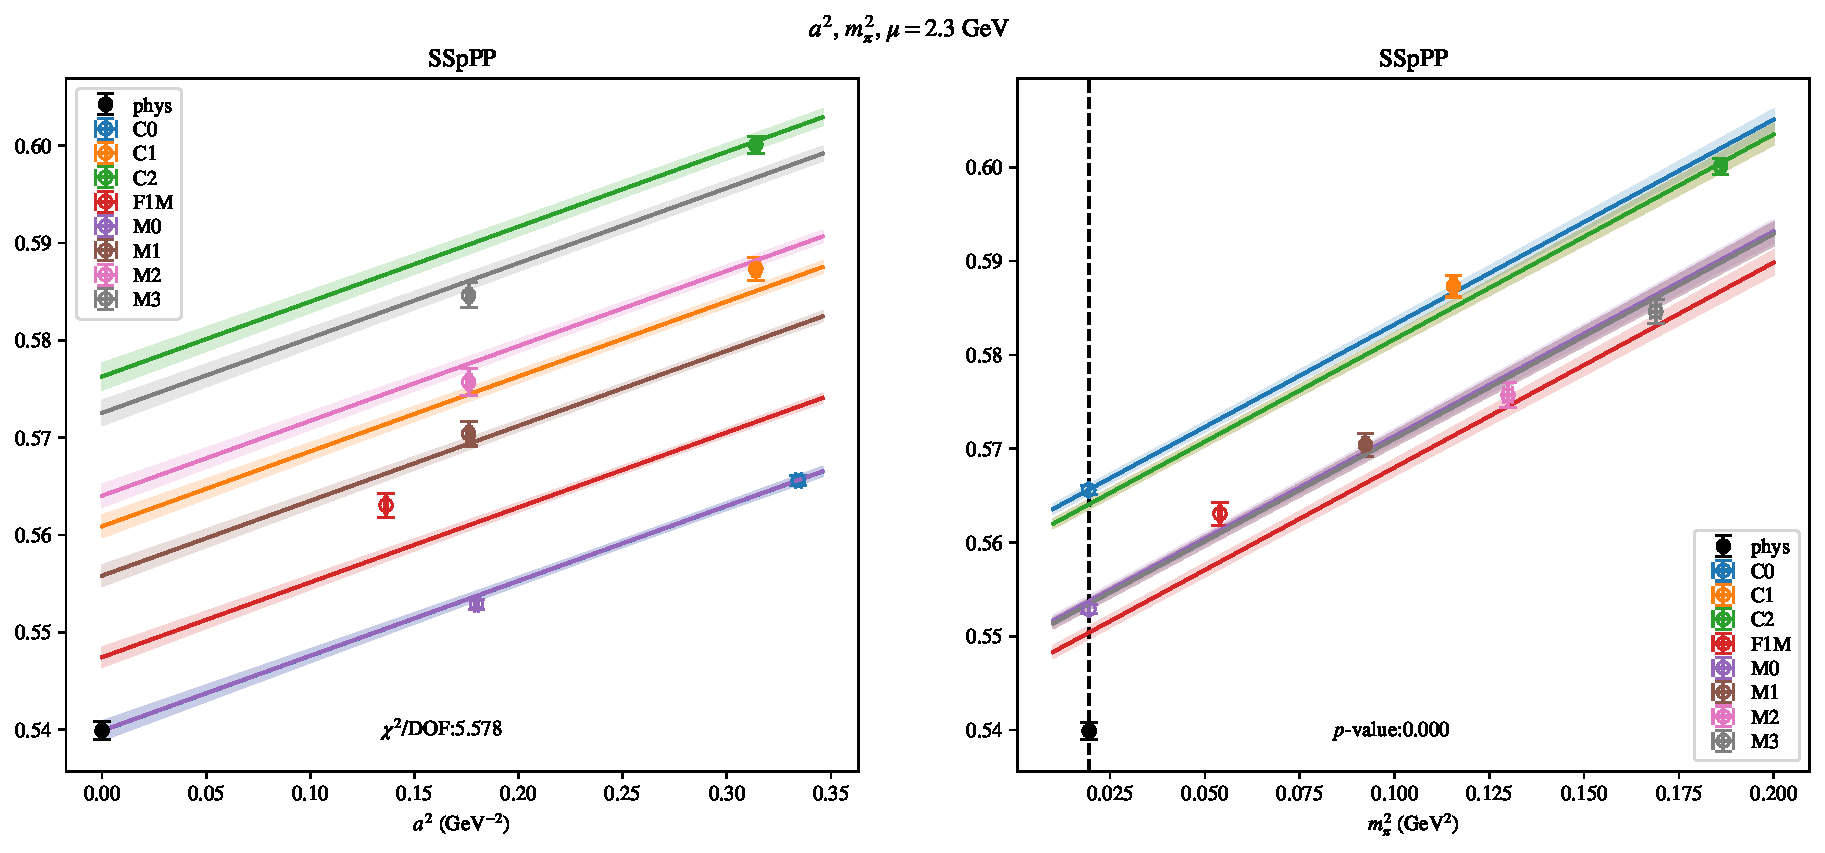
\includepdf[link, pages=-]{VVmAA/SUSY/a2m2_23.pdf}
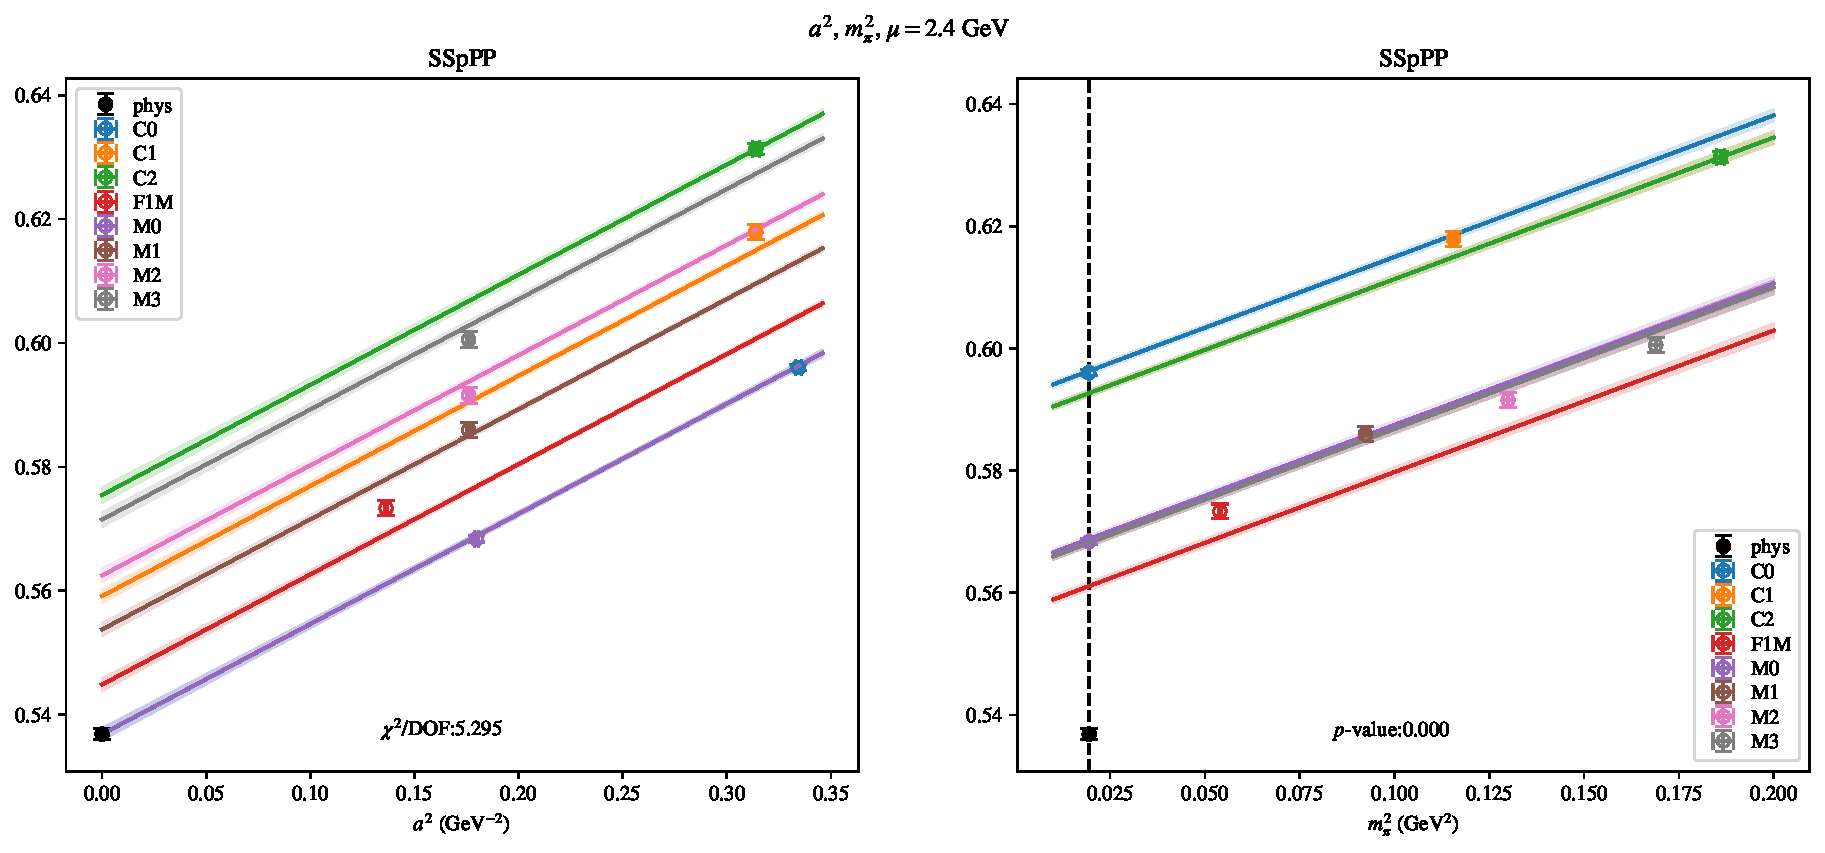
\includepdf[link, pages=-]{VVmAA/SUSY/a2m2_24.pdf}
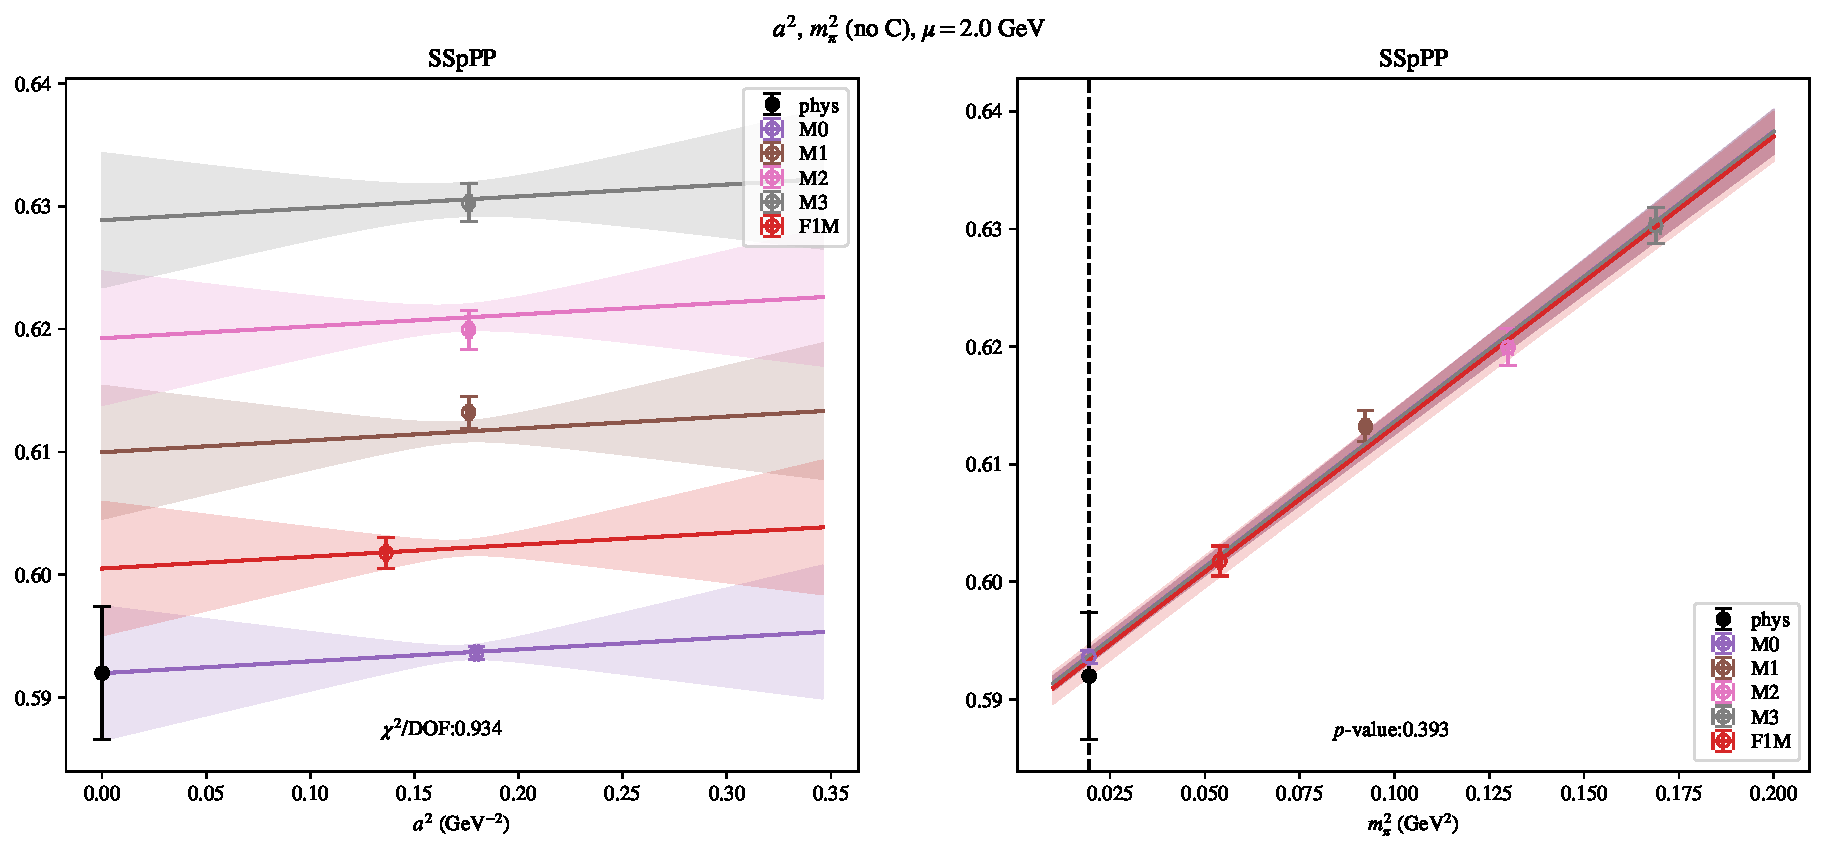
\includepdf[link, pages=-]{VVmAA/SUSY/a2m2noC_20.pdf}
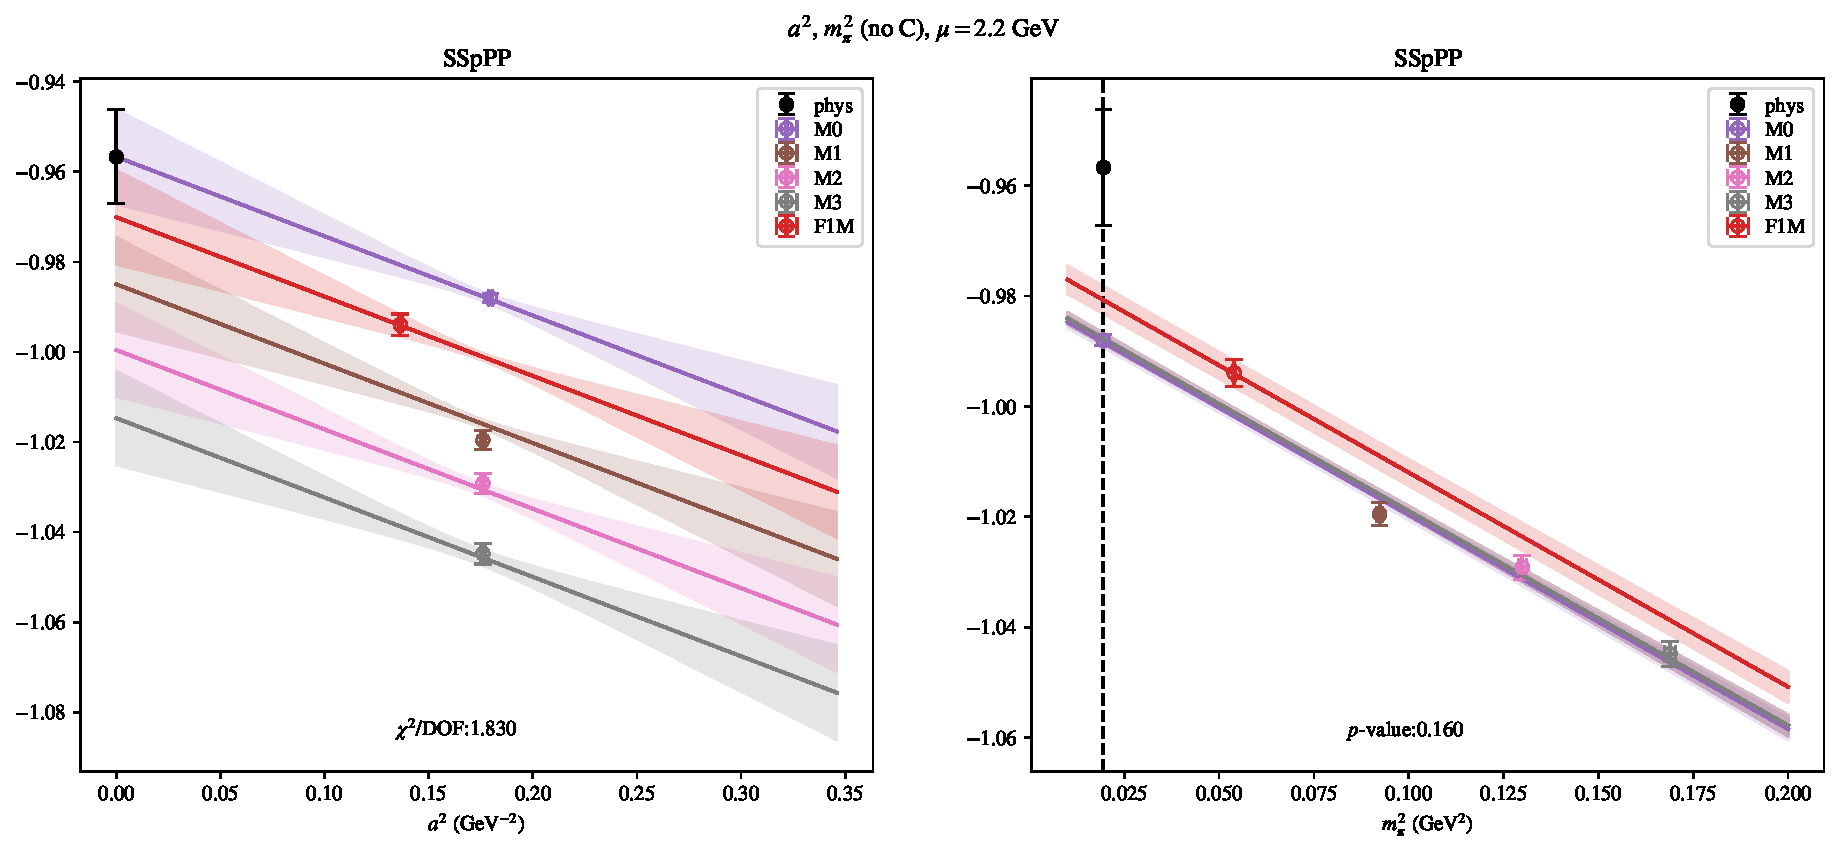
\includepdf[link, pages=-]{VVmAA/SUSY/a2m2noC_22.pdf}
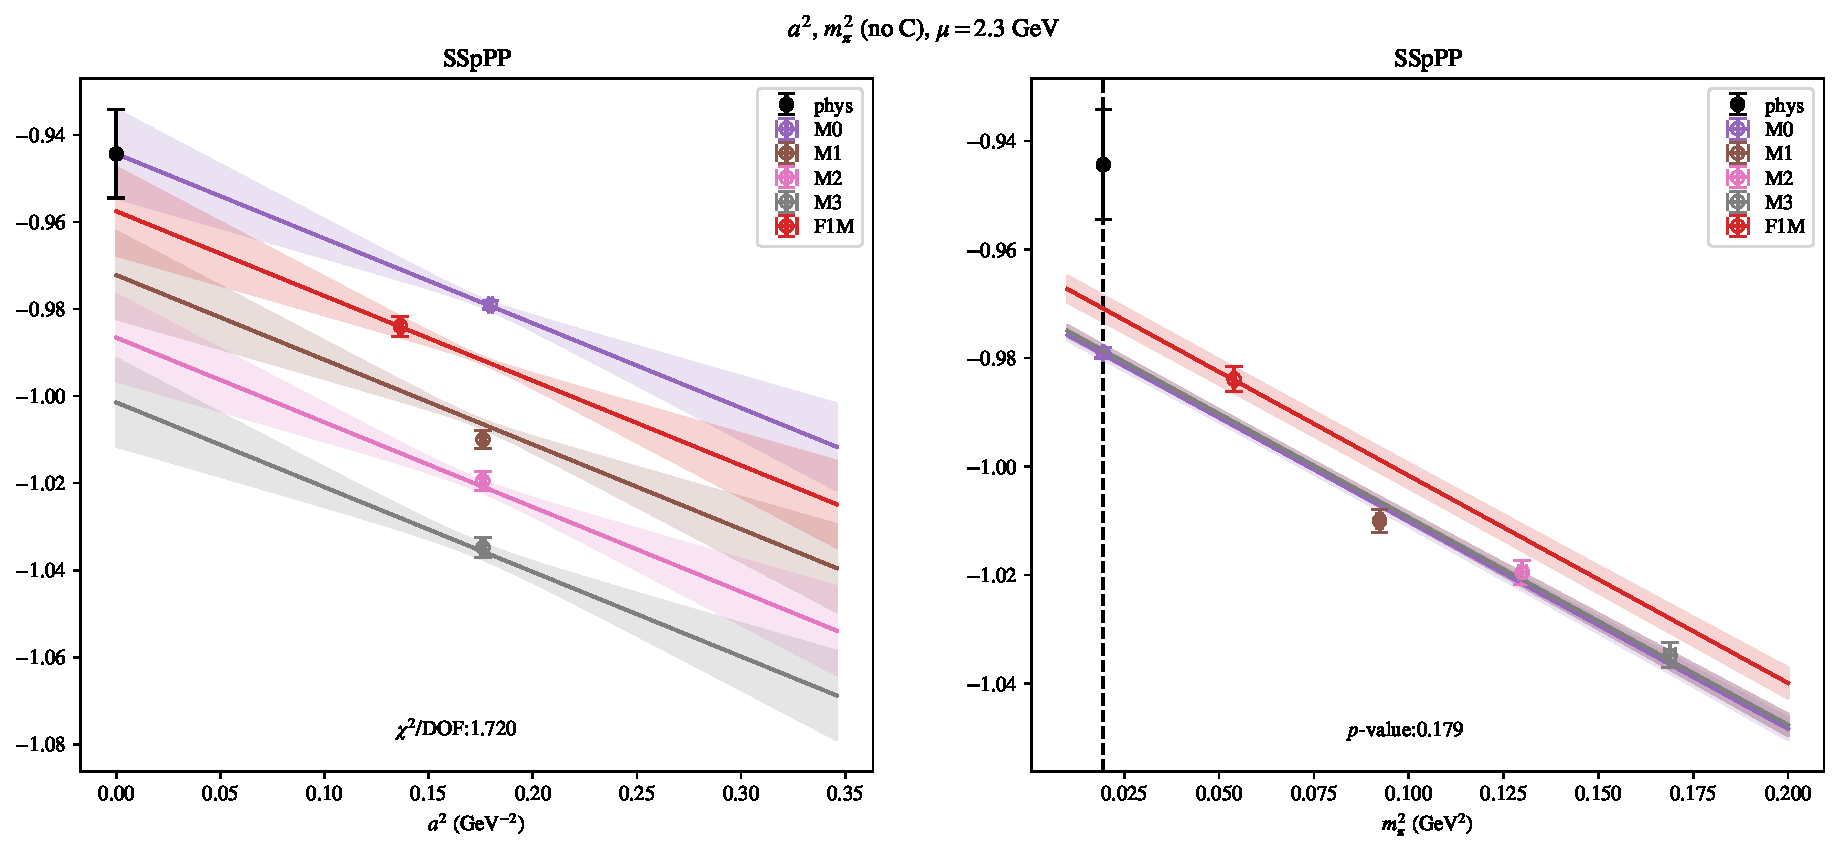
\includepdf[link, pages=-]{VVmAA/SUSY/a2m2noC_23.pdf}
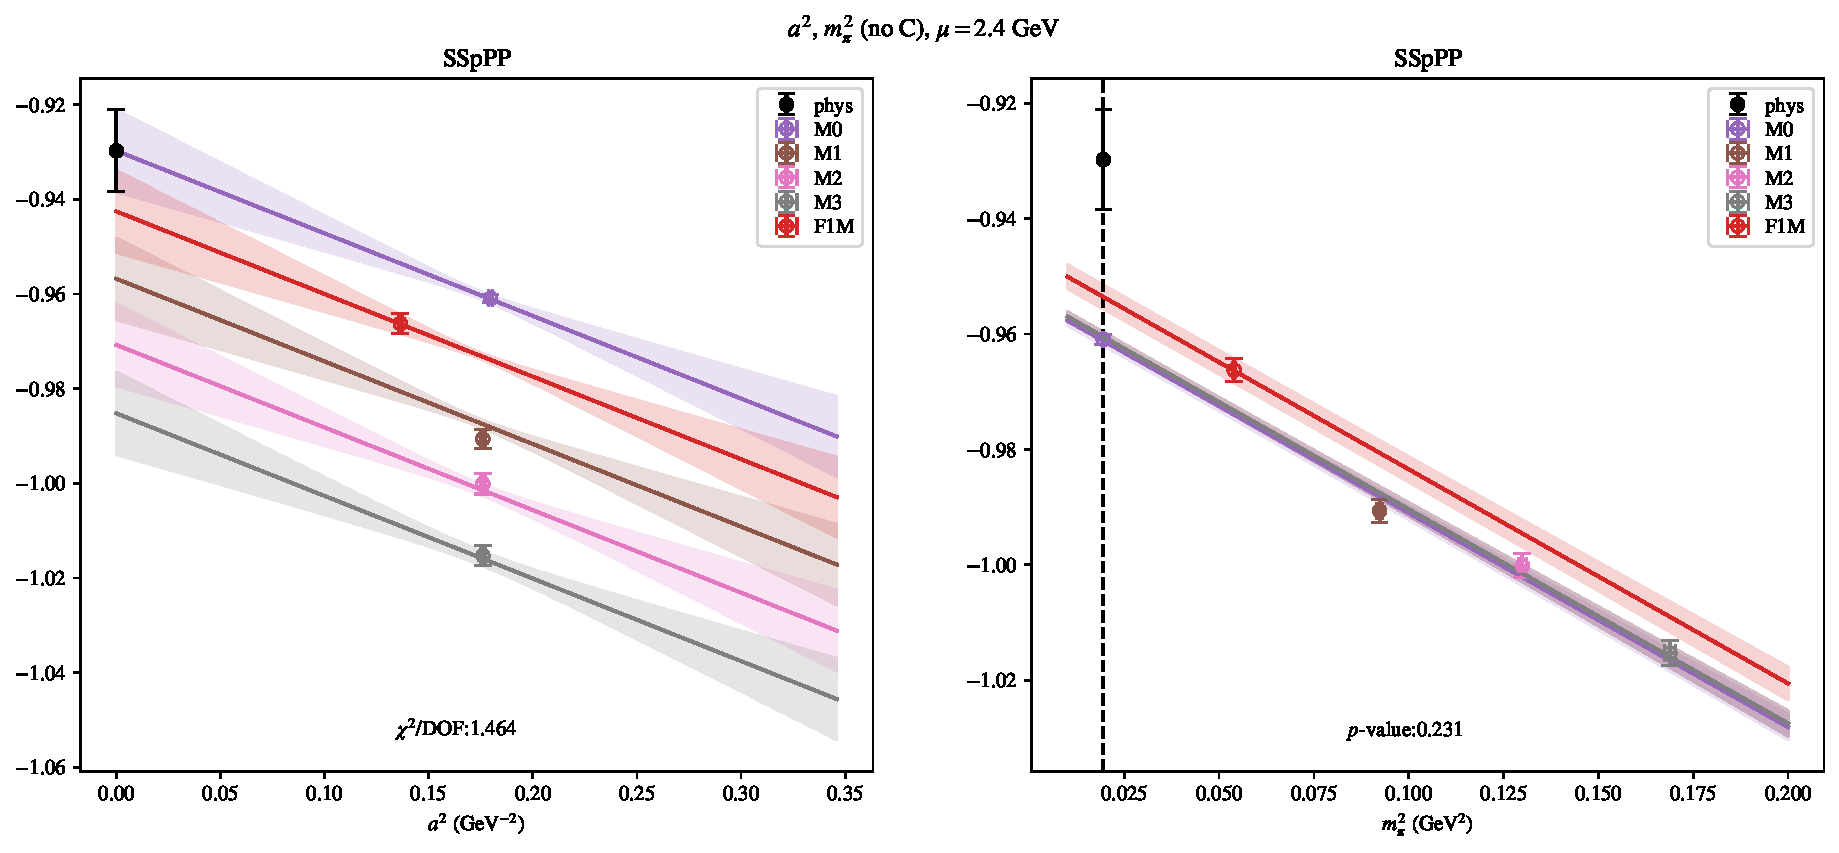
\includepdf[link, pages=-]{VVmAA/SUSY/a2m2noC_24.pdf}
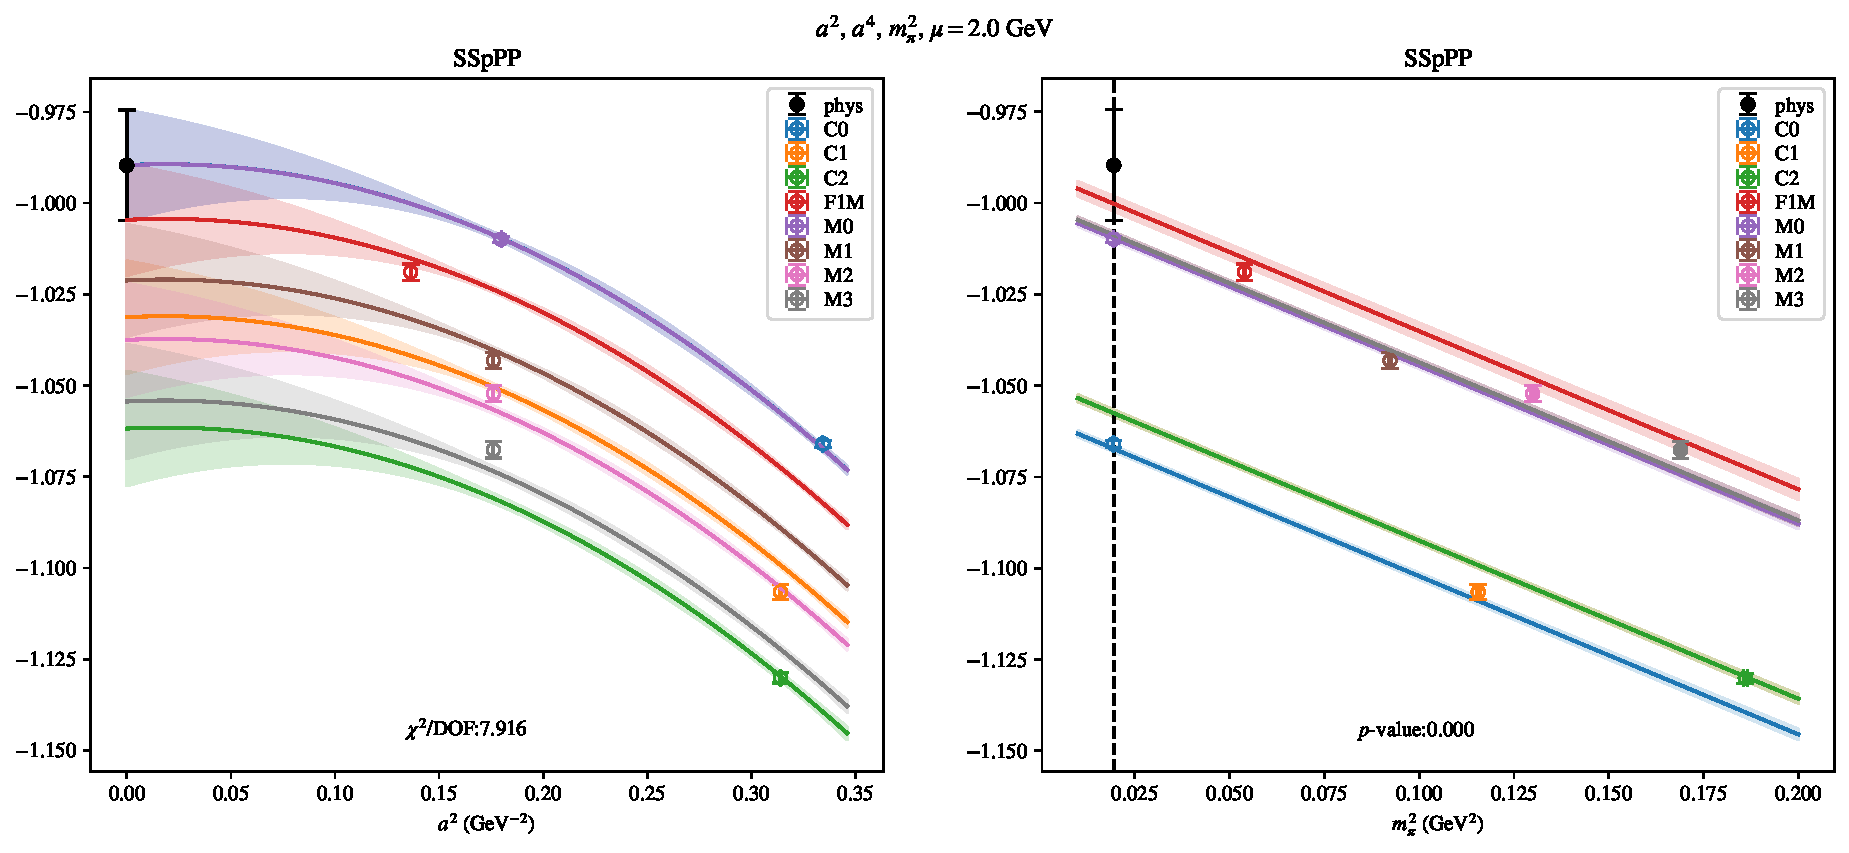
\includepdf[link, pages=-]{VVmAA/SUSY/a2a4m2_20.pdf}
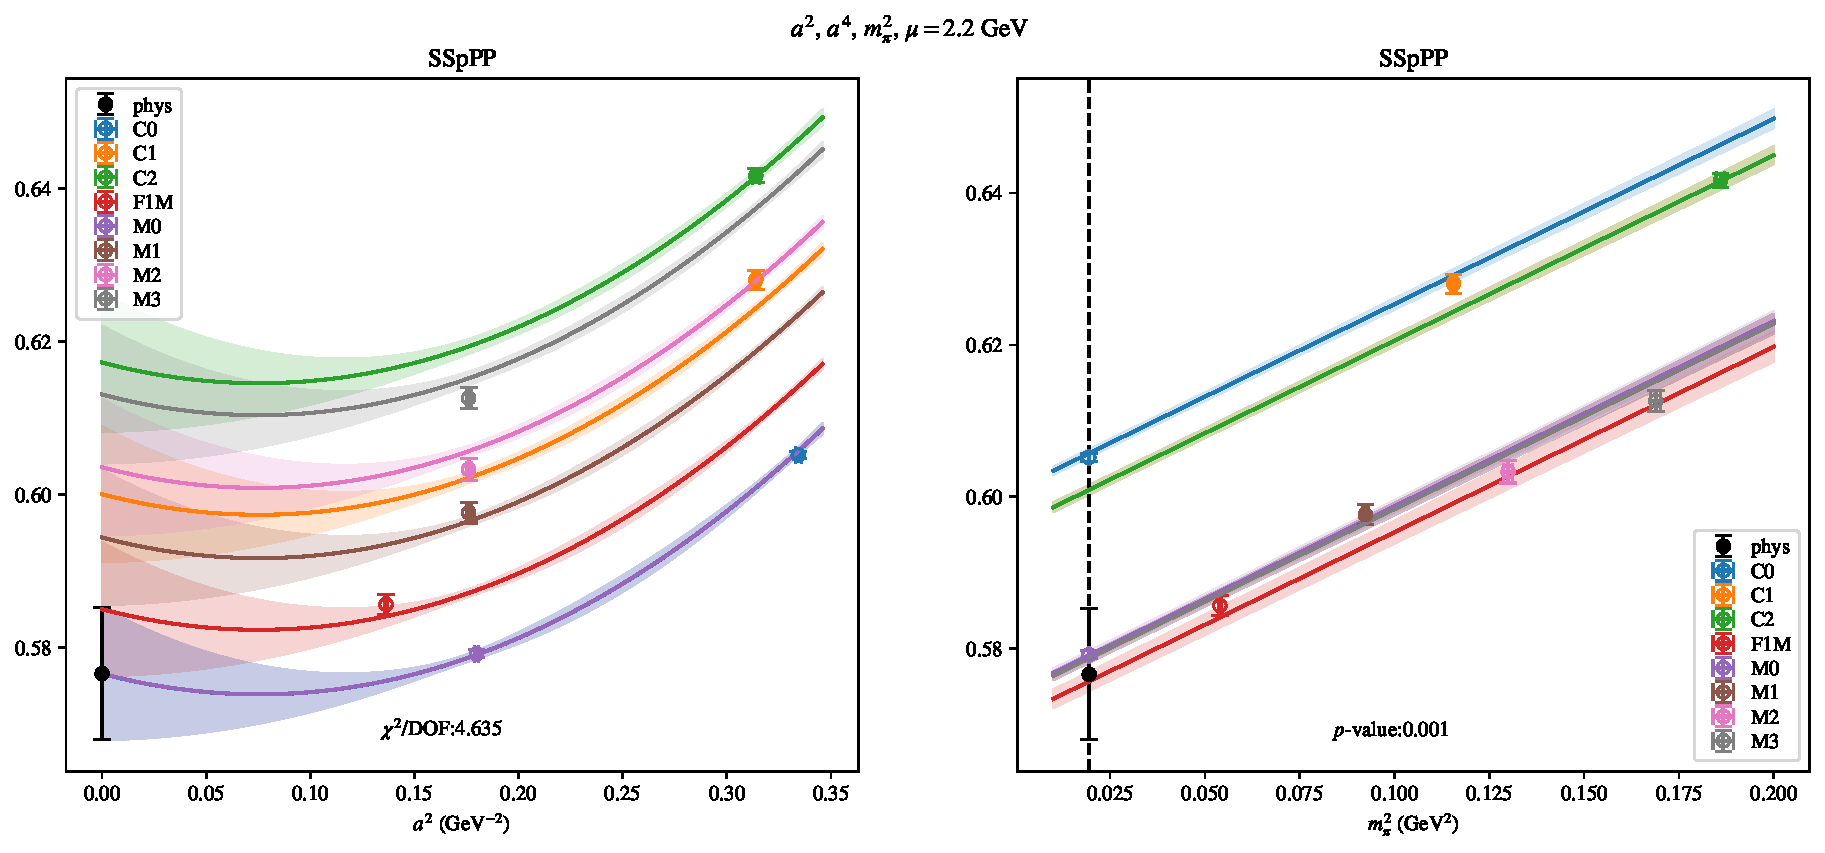
\includepdf[link, pages=-]{VVmAA/SUSY/a2a4m2_22.pdf}
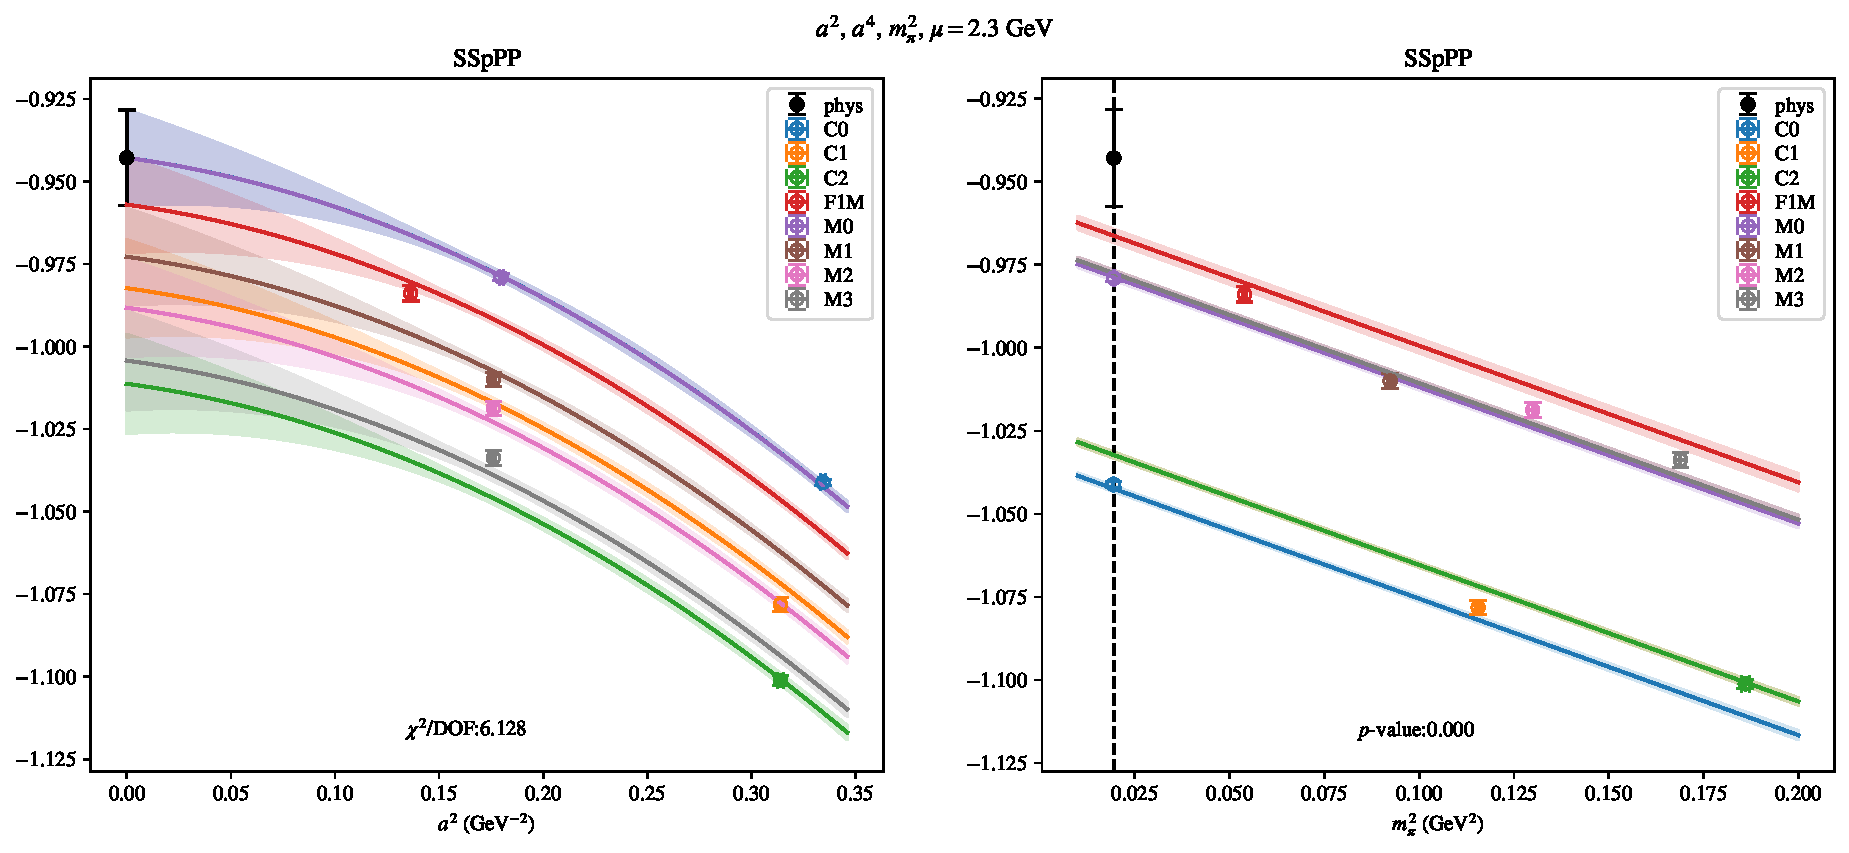
\includepdf[link, pages=-]{VVmAA/SUSY/a2a4m2_23.pdf}
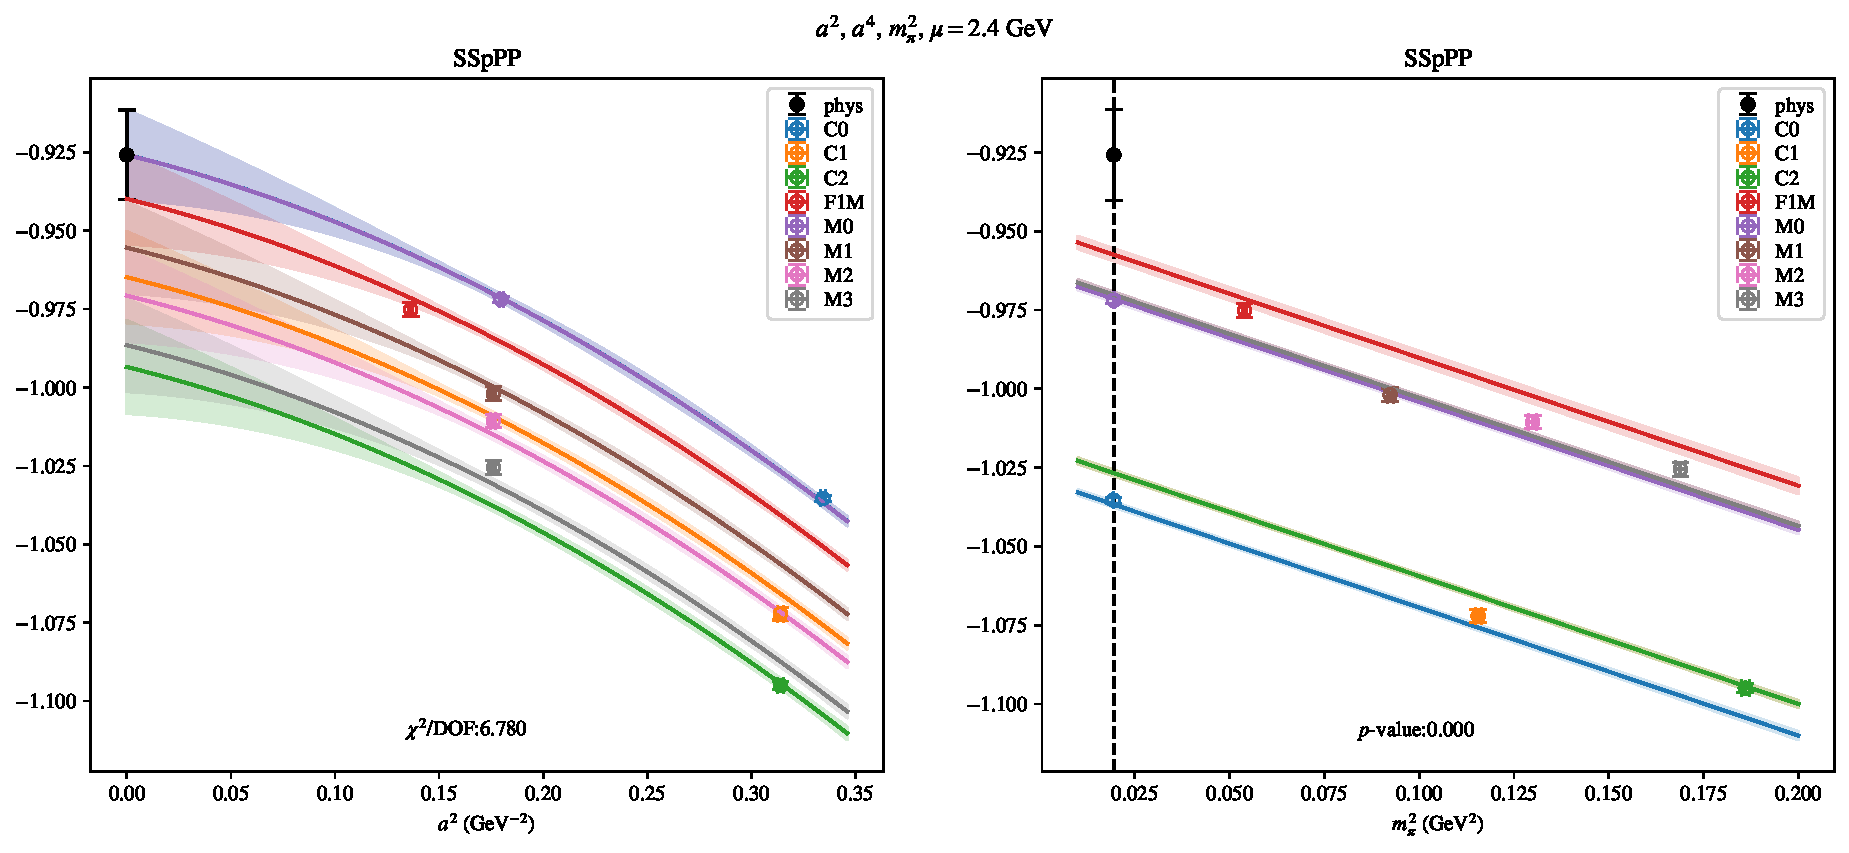
\includepdf[link, pages=-]{VVmAA/SUSY/a2a4m2_24.pdf}
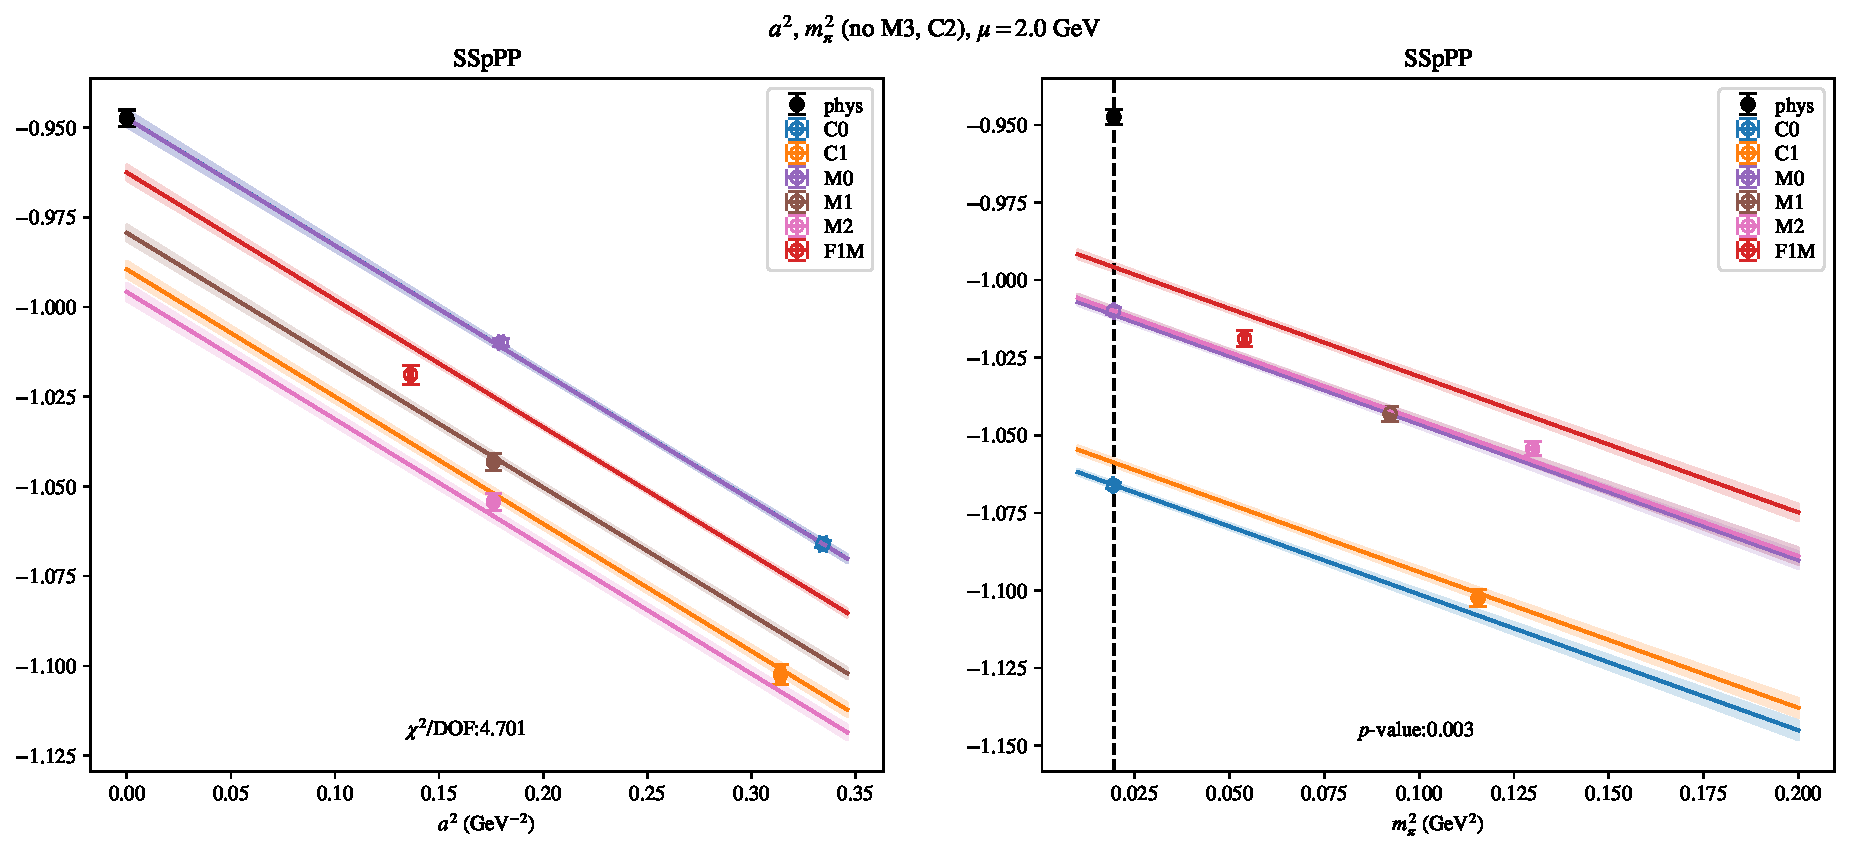
\includepdf[link, pages=-]{VVmAA/SUSY/a2m2mcut_20.pdf}
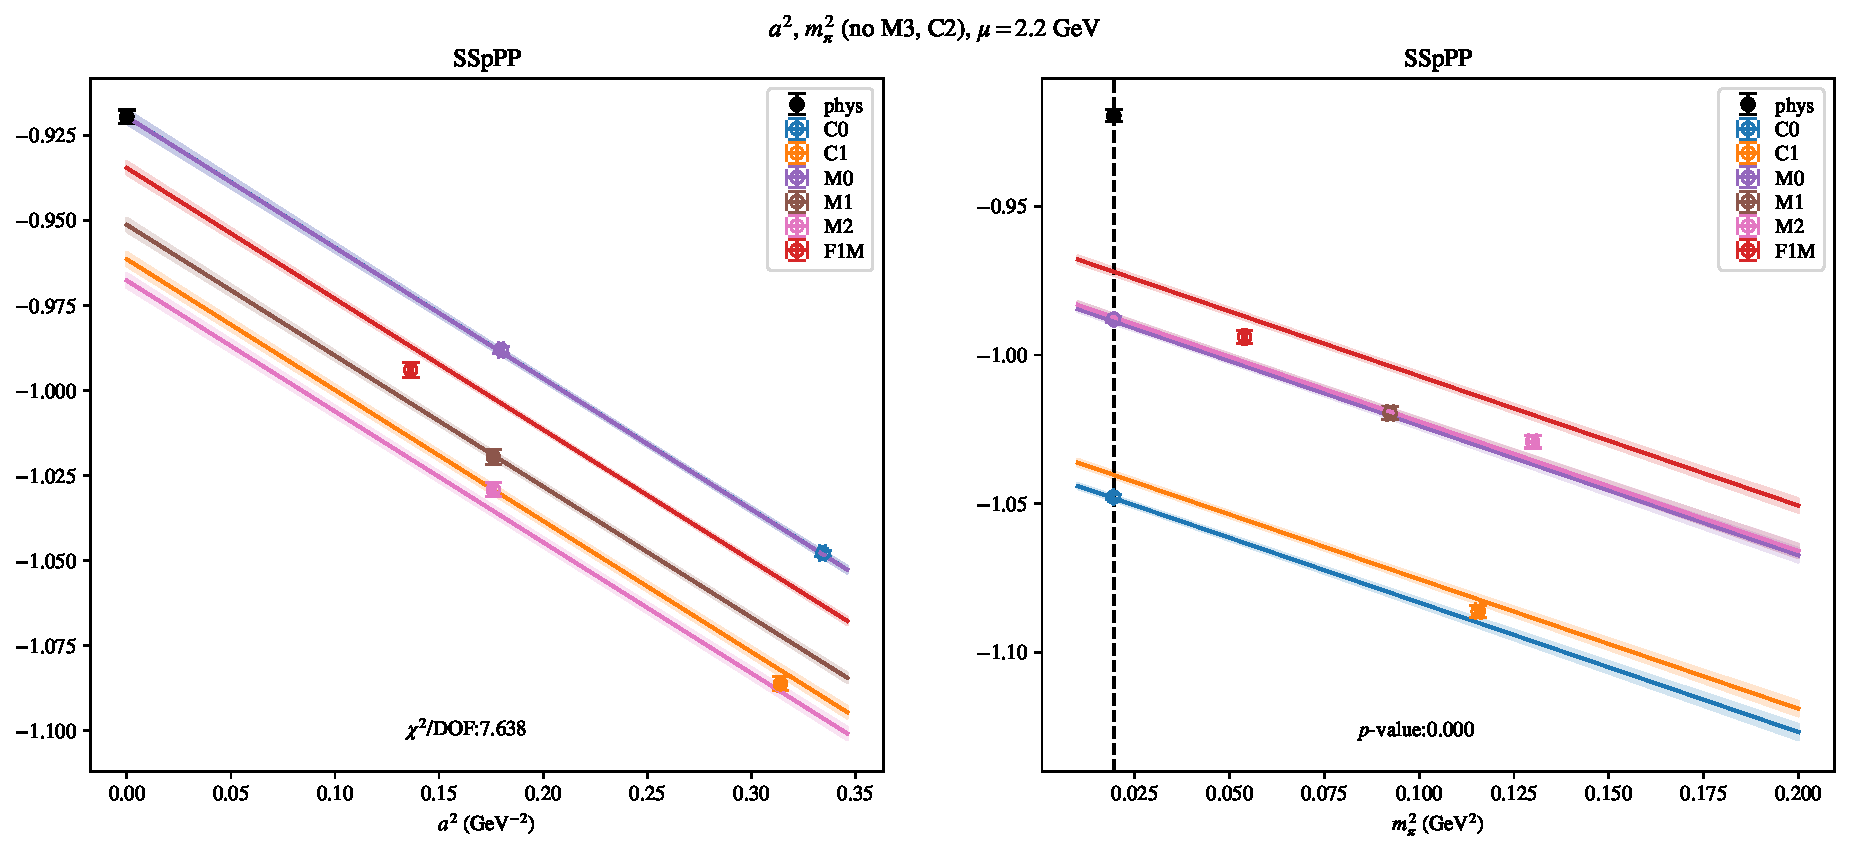
\includepdf[link, pages=-]{VVmAA/SUSY/a2m2mcut_22.pdf}
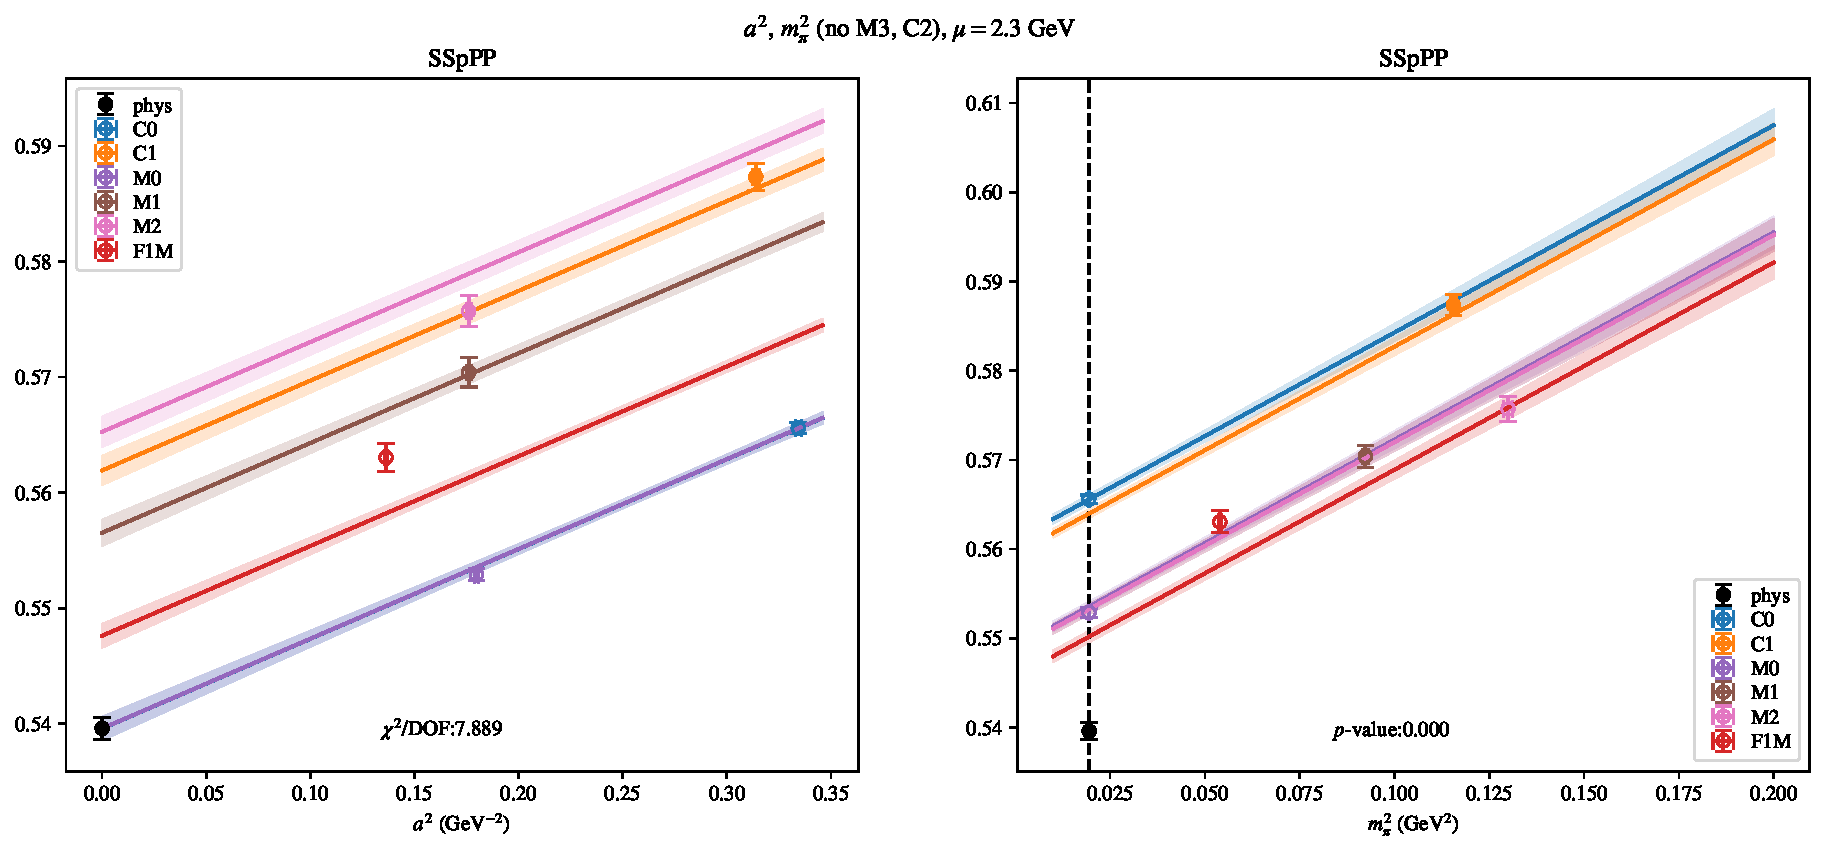
\includepdf[link, pages=-]{VVmAA/SUSY/a2m2mcut_23.pdf}
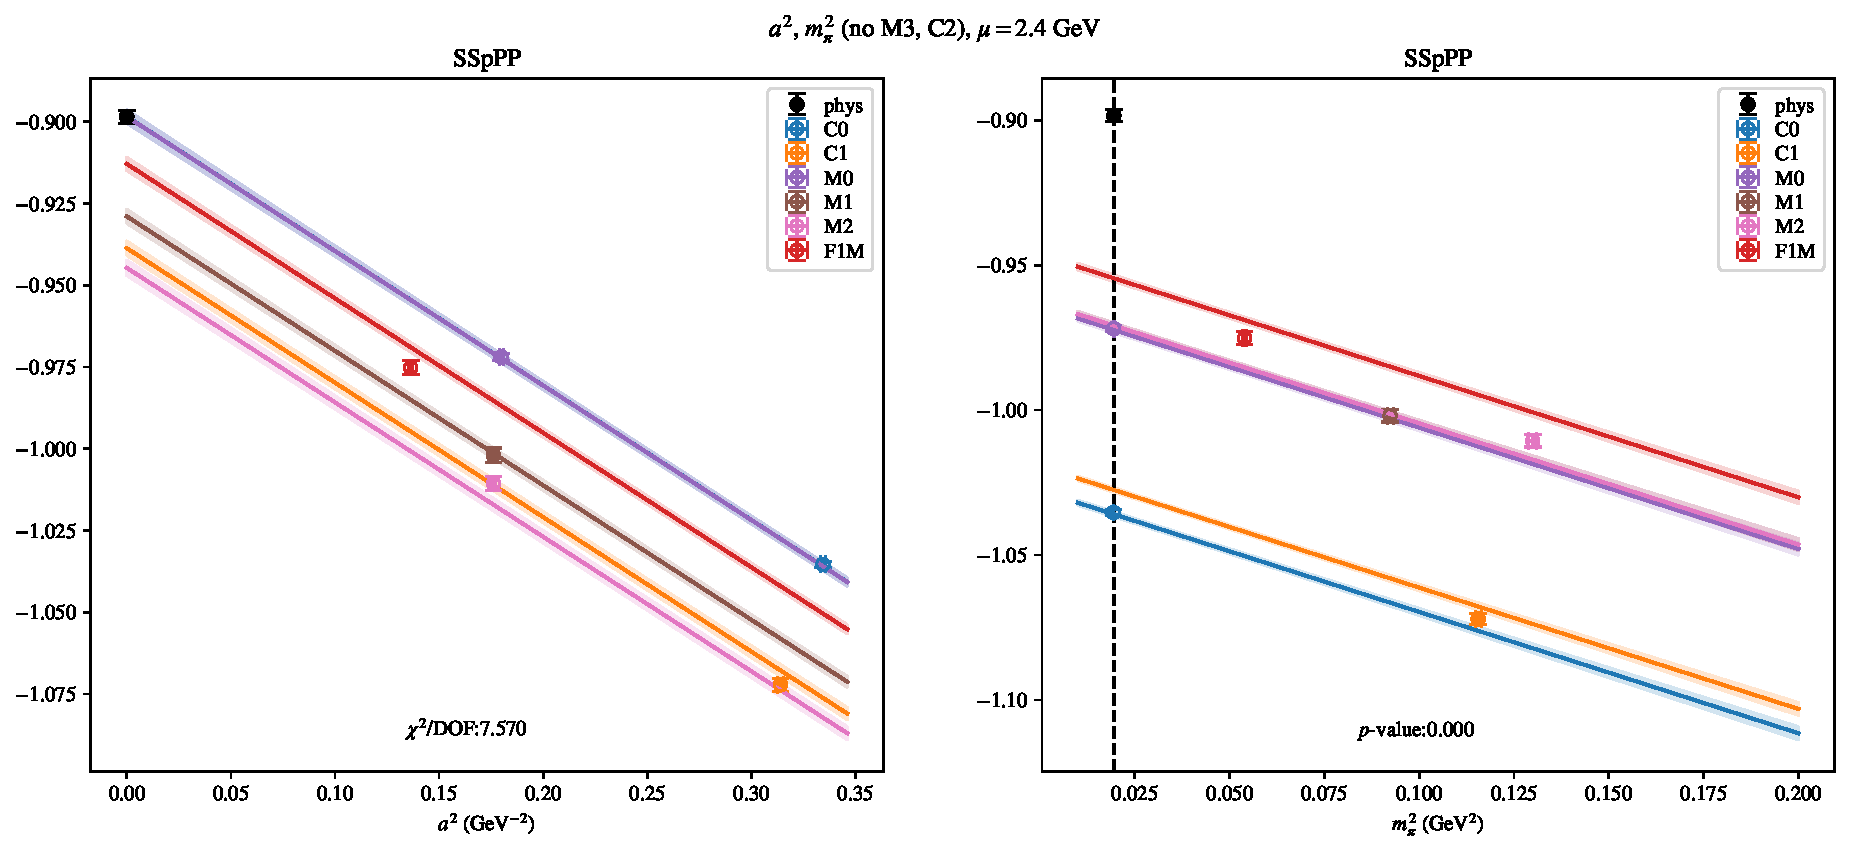
\includepdf[link, pages=-]{VVmAA/SUSY/a2m2mcut_24.pdf}
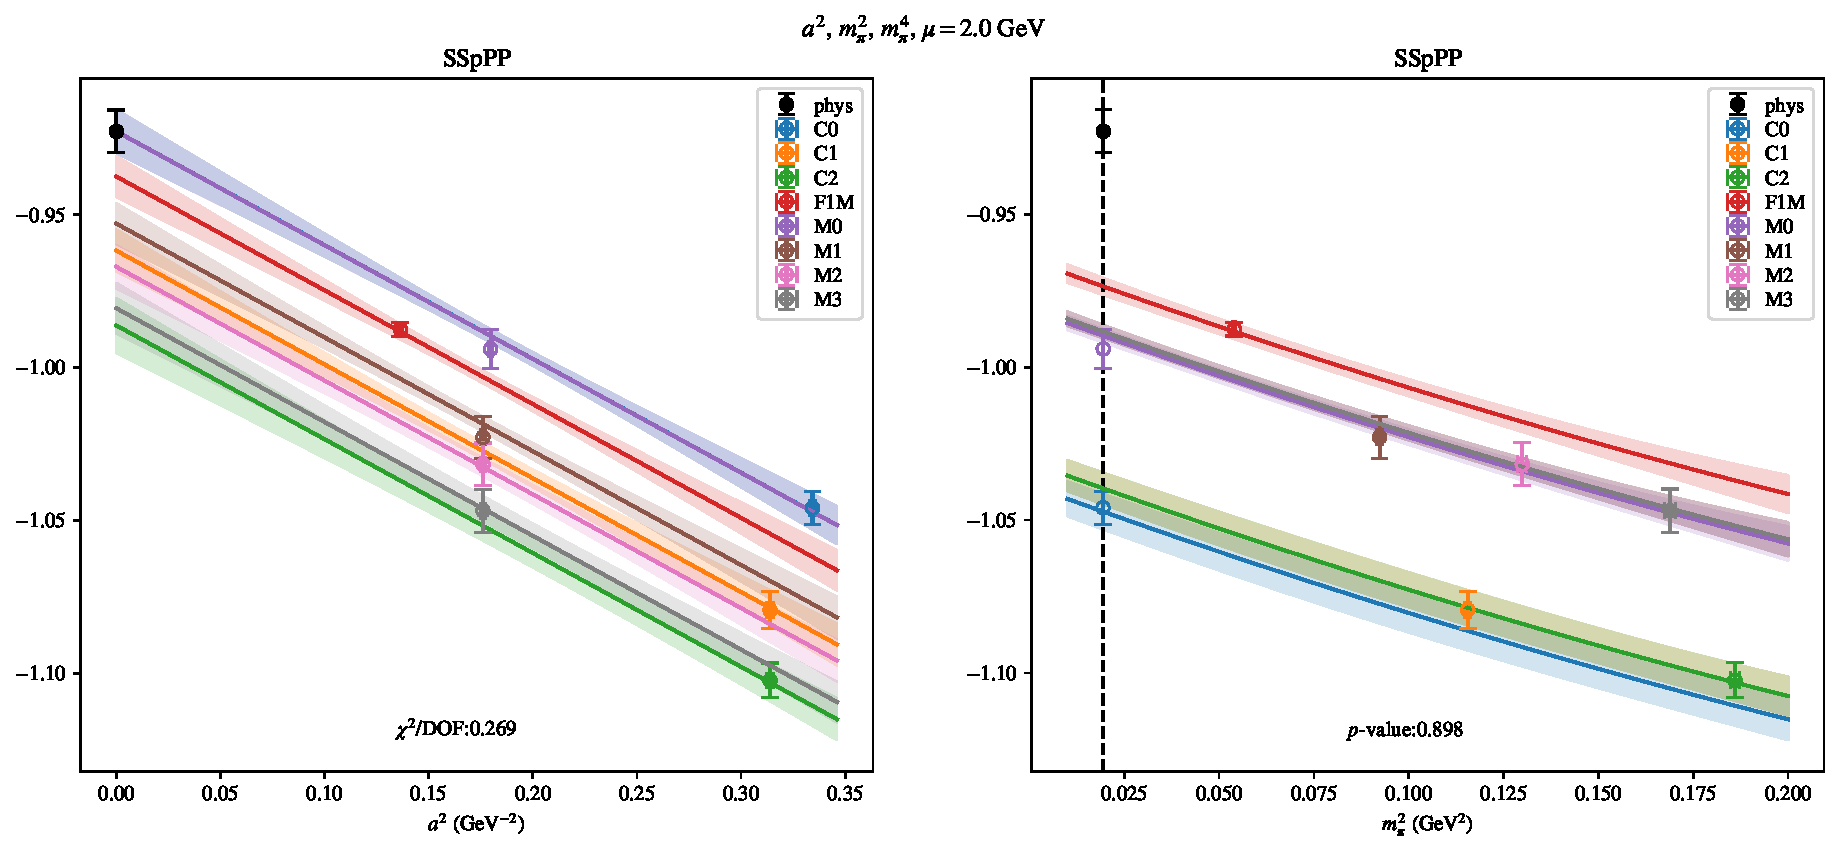
\includepdf[link, pages=-]{VVmAA/SUSY/a2m2m4_20.pdf}
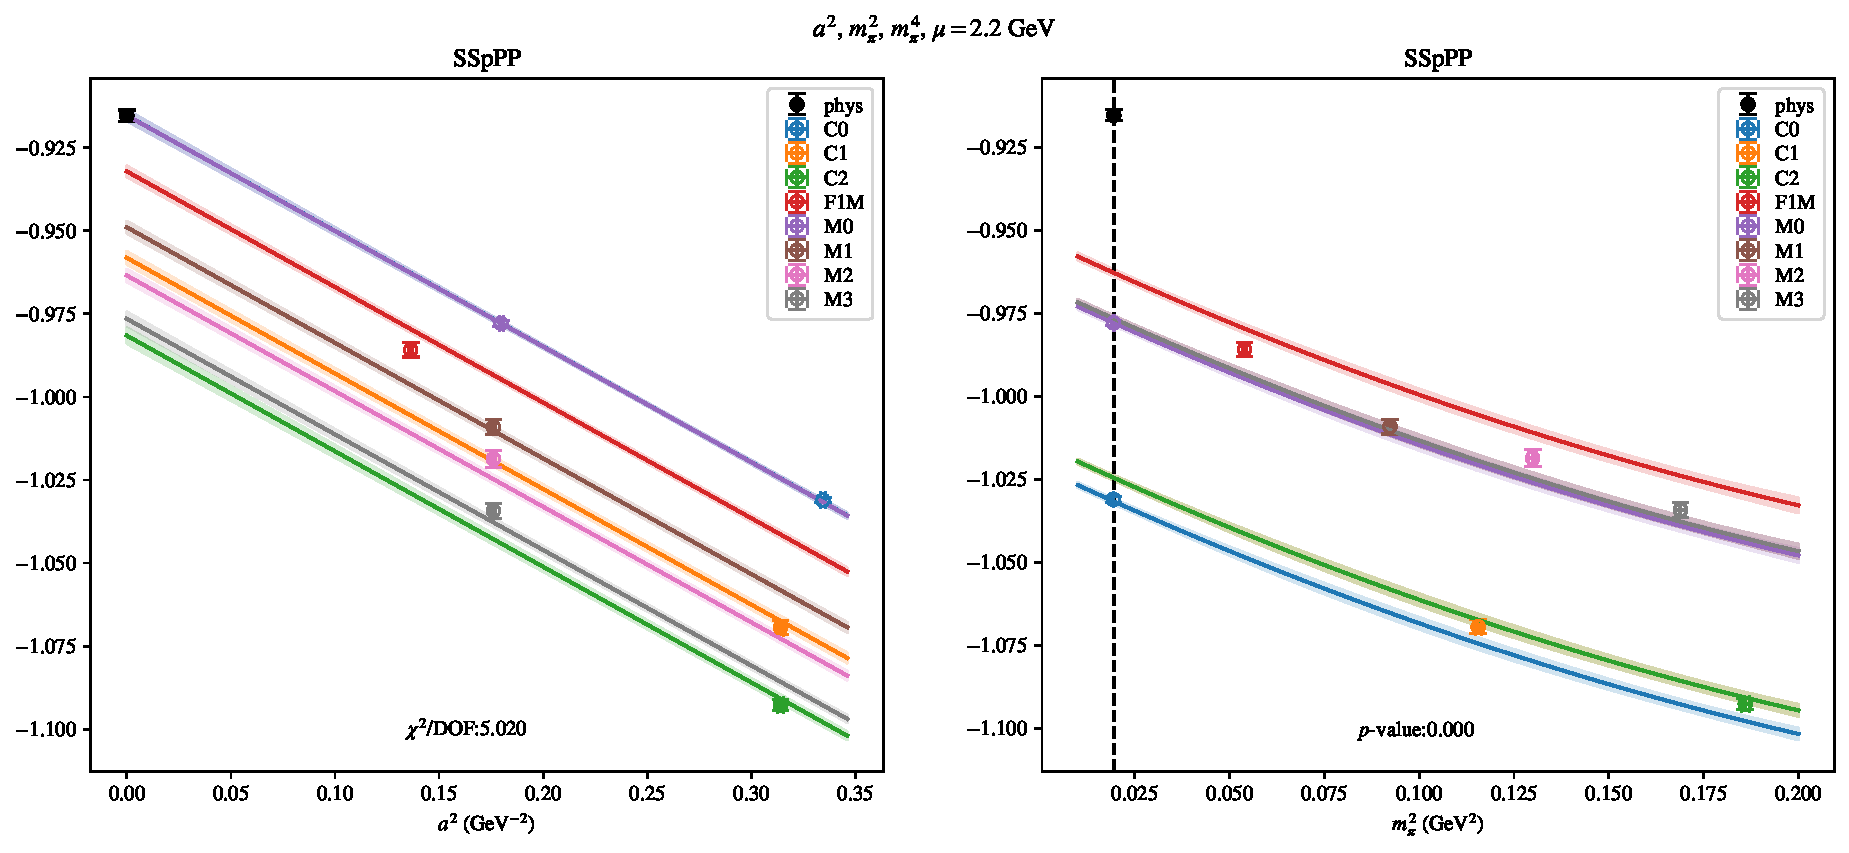
\includepdf[link, pages=-]{VVmAA/SUSY/a2m2m4_22.pdf}
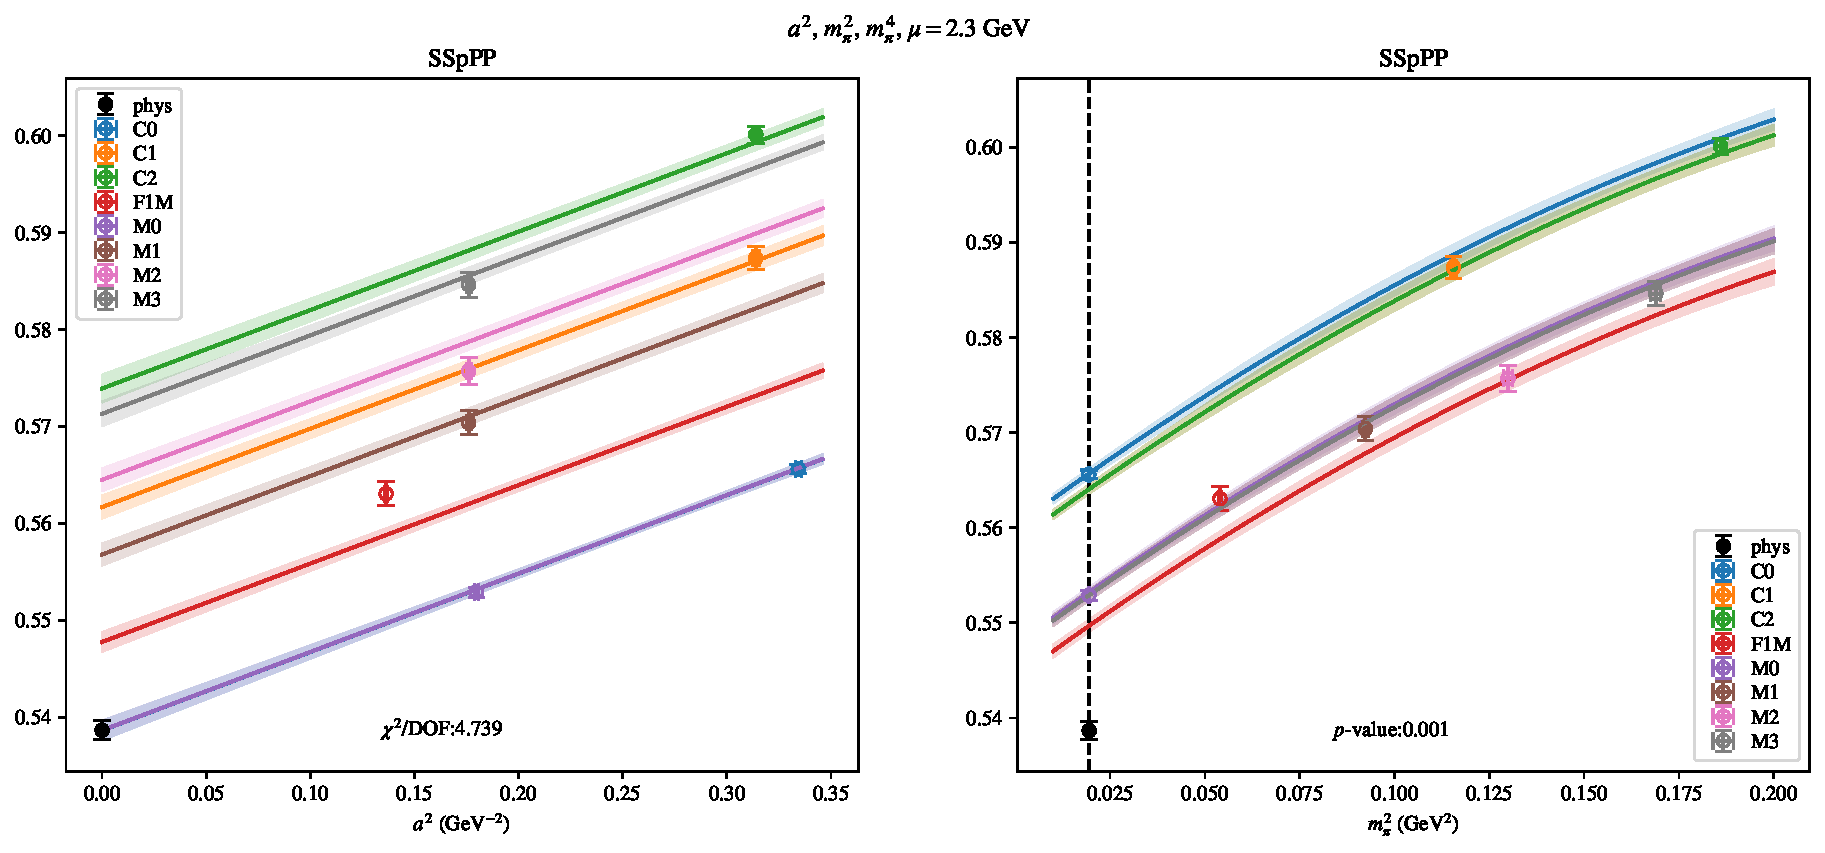
\includepdf[link, pages=-]{VVmAA/SUSY/a2m2m4_23.pdf}
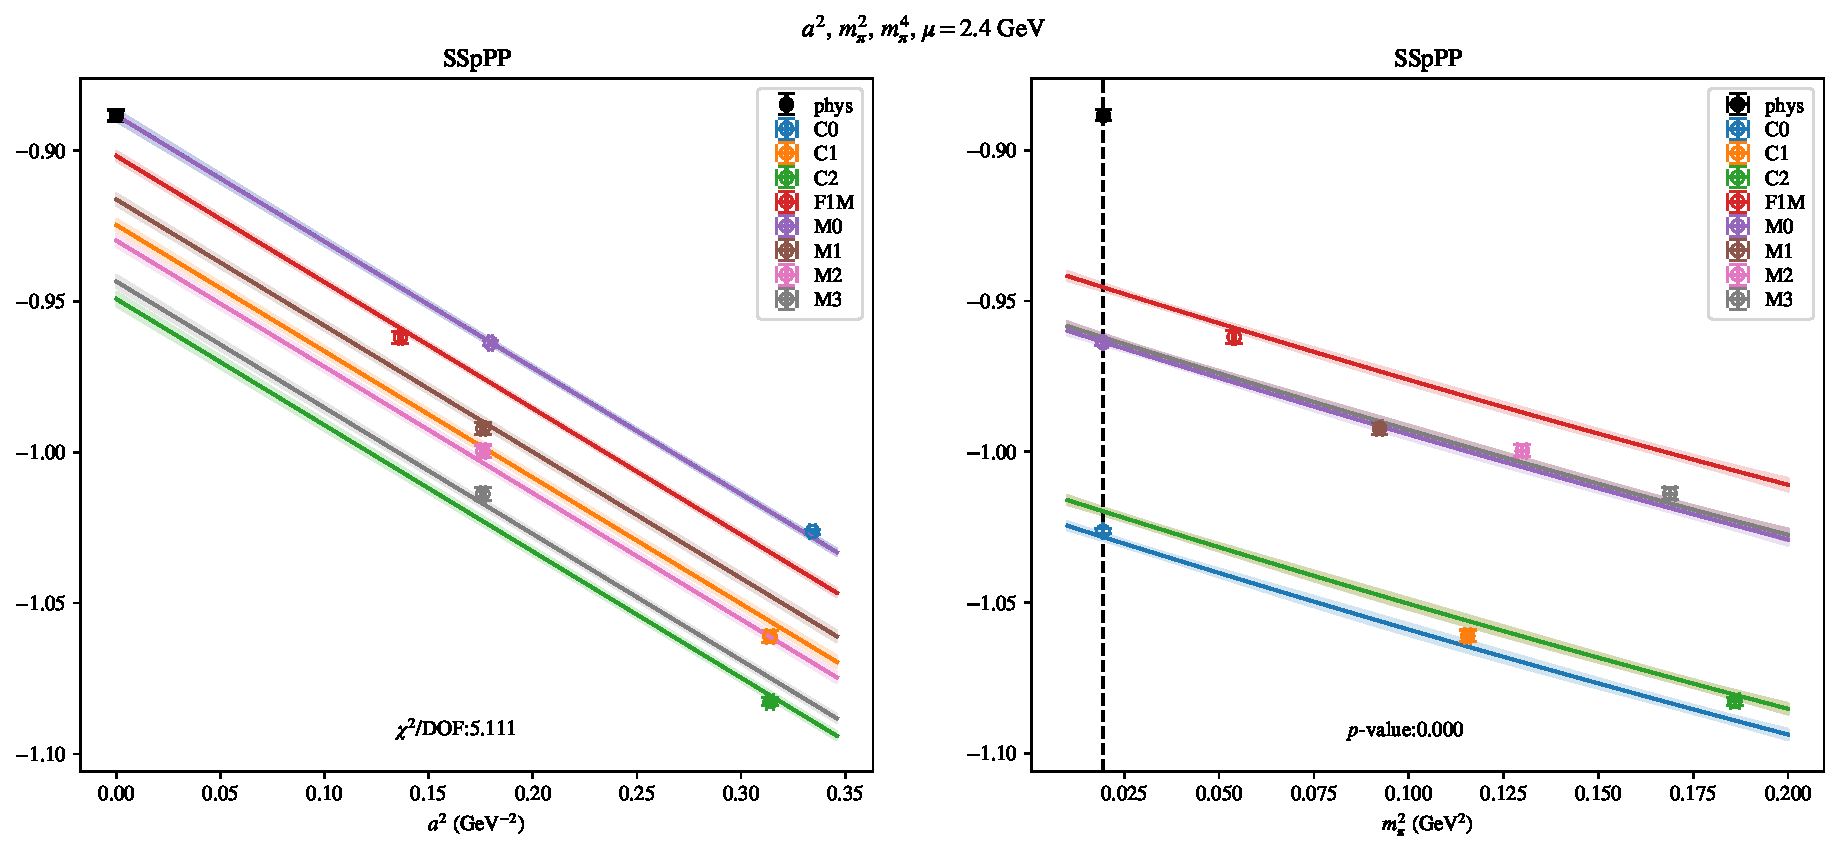
\includepdf[link, pages=-]{VVmAA/SUSY/a2m2m4_24.pdf}
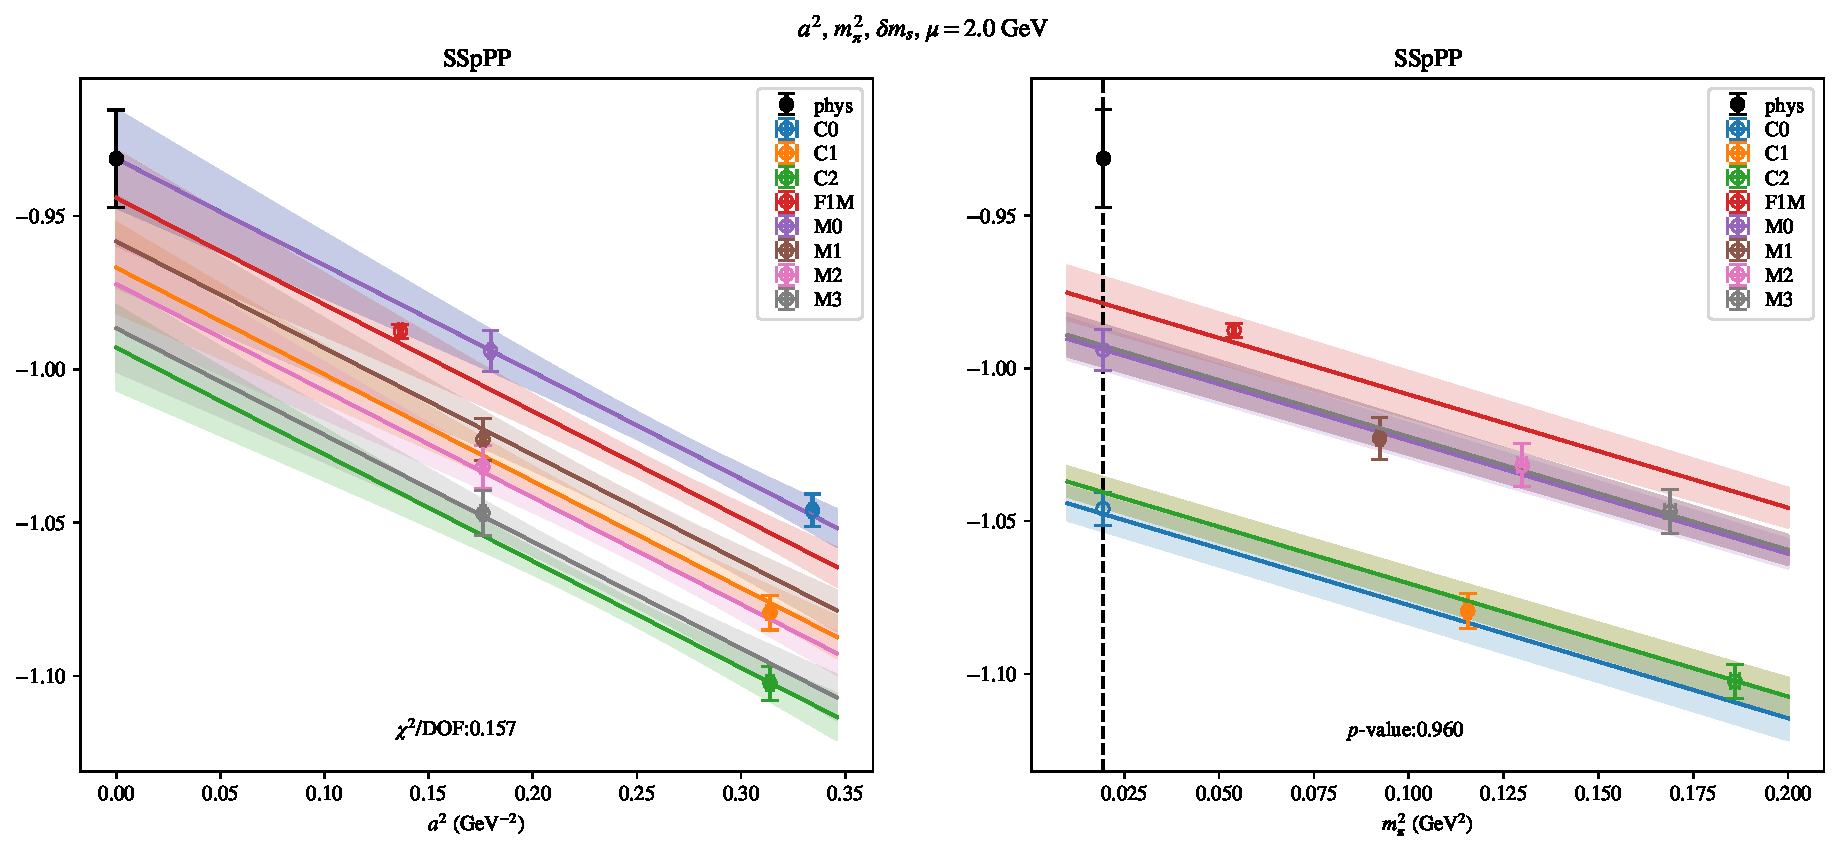
\includepdf[link, pages=-]{VVmAA/SUSY/a2m2delm_20.pdf}
\includepdf[link, pages=-]{VVmAA/SUSY/a2m2delm_22.pdf}
\includepdf[link, pages=-]{VVmAA/SUSY/a2m2delm_23.pdf}
\includepdf[link, pages=-]{VVmAA/SUSY/a2m2delm_24.pdf}
\clearpage
\section{$\mathcal{B}_3$}
\begin{table}[h!]
\begin{center}
\begin{tabular}{|c|c|c|c|c|c|c|}
\hline
$\mu$ (GeV) & $a^2$, $m_\pi^2$& $a^2$, $m_\pi^2$ (no C)& $a^2$, $m_\pi^2$, $a^4$& $a^2$, $m_\pi^2$ (no M3, C2)& $a^2$, $m_\pi^2$, $m_\pi^4$& $a^2$, $m_\pi^2$, $\delta m_s$\\
\hline
2.0& \hyperlink{SSmPP/SUSY/a2m2_20.pdf.1}{\textbf{0.28133(58)}: 4.465 (0.0)} & \hyperlink{SSmPP/SUSY/a2m2noC_20.pdf.1}{\textbf{0.2843(29)}: 4.506 (0.011)} & \hyperlink{SSmPP/SUSY/a2a4m2_20.pdf.1}{\textbf{0.2803(48)}: 5.572 (0.0)} & \hyperlink{SSmPP/SUSY/a2m2mcut_20.pdf.1}{\textbf{0.28126(63)}: 4.879 (0.002)} & \hyperlink{SSmPP/SUSY/a2m2m4_20.pdf.1}{\textbf{0.28075(64)}: 3.82 (0.004)} & \hyperlink{SSmPP/SUSY/a2m2delm_20.pdf.1}{\textbf{0.28125(61)}: 5.451 (0.0)}\\
2.2& \hyperlink{SSmPP/SUSY/a2m2_22.pdf.1}{\textbf{0.27295(54)}: 6.095 (0.0)} & \hyperlink{SSmPP/SUSY/a2m2noC_22.pdf.1}{\textbf{0.2764(29)}: 3.746 (0.024)} & \hyperlink{SSmPP/SUSY/a2a4m2_22.pdf.1}{\textbf{0.2736(47)}: 7.602 (0.0)} & \hyperlink{SSmPP/SUSY/a2m2mcut_22.pdf.1}{\textbf{0.27287(61)}: 5.749 (0.001)} & \hyperlink{SSmPP/SUSY/a2m2m4_22.pdf.1}{\textbf{0.27258(66)}: 5.931 (0.0)} & \hyperlink{SSmPP/SUSY/a2m2delm_22.pdf.1}{\textbf{0.27282(56)}: 7.202 (0.0)}\\
2.3& \hyperlink{SSmPP/SUSY/a2m2_23.pdf.1}{\textbf{0.26905(52)}: 6.779 (0.0)} & \hyperlink{SSmPP/SUSY/a2m2noC_23.pdf.1}{\textbf{0.2737(27)}: 4.005 (0.018)} & \hyperlink{SSmPP/SUSY/a2a4m2_23.pdf.1}{\textbf{0.2713(47)}: 8.399 (0.0)} & \hyperlink{SSmPP/SUSY/a2m2mcut_23.pdf.1}{\textbf{0.26897(61)}: 6.92 (0.0)} & \hyperlink{SSmPP/SUSY/a2m2m4_23.pdf.1}{\textbf{0.26867(63)}: 6.746 (0.0)} & \hyperlink{SSmPP/SUSY/a2m2delm_23.pdf.1}{\textbf{0.26886(54)}: 7.8 (0.0)}\\
2.4& \hyperlink{SSmPP/SUSY/a2m2_24.pdf.1}{\textbf{0.26567(51)}: 7.584 (0.0)} & \hyperlink{SSmPP/SUSY/a2m2noC_24.pdf.1}{\textbf{0.2708(26)}: 3.99 (0.018)} & \hyperlink{SSmPP/SUSY/a2a4m2_24.pdf.1}{\textbf{0.2680(47)}: 9.421 (0.0)} & \hyperlink{SSmPP/SUSY/a2m2mcut_24.pdf.1}{\textbf{0.26566(60)}: 8.078 (0.0)} & \hyperlink{SSmPP/SUSY/a2m2m4_24.pdf.1}{\textbf{0.26533(62)}: 7.994 (0.0)} & \hyperlink{SSmPP/SUSY/a2m2delm_24.pdf.1}{\textbf{0.26547(53)}: 8.724 (0.0)}\\
\hline
\end{tabular}
\caption{Physical point value from chiral and continuum extrapolation at renormalisation scale $\mu$. Entries are \textbf{value(error)}: $\chi^2/\text{DOF}$ ($p$-value).}
\end{center}
\end{table}
\begin{table}[h!]
\begin{center}
\begin{tabular}{|c c|c|c|c|c|c|c|}
\hline
$\mu$ (GeV) &  & $a^2$, $m_\pi^2$& $a^2$, $m_\pi^2$ (no C)& $a^2$, $m_\pi^2$, $a^4$& $a^2$, $m_\pi^2$ (no M3, C2)& $a^2$, $m_\pi^2$, $m_\pi^4$& $a^2$, $m_\pi^2$, $\delta m_s$\\
\hline
\multirow{3}{0.5in}{2.0} & $\alpha$ & 0.650(10)& 0.587(65)& 0.68(16)& 0.650(10)& 0.658(10)& 0.651(10)\\
 & $\beta$ & 0.00656(34)& 0.00597(48)& 0.00657(35)& 0.00703(47)& 0.0085(11)& 0.00659(35)\\
 & $\gamma$ &  &  & -0.061&  & -0.00018(88)& -0.001(25)\\
\hline
\multirow{3}{0.5in}{2.2} & $\alpha$ & 0.7591(89)& 0.681(66)& 0.73(17)& 0.759(10)& 0.764(10)& 0.7612(92)\\
 & $\beta$ & 0.00726(23)& 0.00679(30)& 0.00725(25)& 0.00758(47)& 0.0086(12)& 0.00731(24)\\
 & $\gamma$ &  &  & 0.046&  & -0.00012(99)& -0.002(24)\\
\hline
\multirow{3}{0.5in}{2.3} & $\alpha$ & 0.8158(90)& 0.707(65)& 0.73(17)& 0.816(11)& 0.821(10)& 0.8189(93)\\
 & $\beta$ & 0.00744(22)& 0.00691(29)& 0.00740(25)& 0.00773(44)& 0.0087(12)& 0.00752(23)\\
 & $\gamma$ &  &  & 0.15(31)&  & -0.00012(98)& -0.003(24)\\
\hline
\multirow{3}{0.5in}{2.4} & $\alpha$ & 0.8677(90)& 0.746(64)& 0.78(17)& 0.867(11)& 0.873(10)& 0.8712(93)\\
 & $\beta$ & 0.00763(22)& 0.00700(28)& 0.00759(25)& 0.00789(40)& 0.0088(11)& 0.00773(23)\\
 & $\gamma$ &  &  & 0.15(32)&  & -0.00011(94)& -0.003(24)\\
\hline
\end{tabular}
\caption{Fit values of coefficients in $Q = Q_{phys} + \mathbf{\alpha} a^2 + \mathbf{\beta}\left(\frac{m_\pi^2}{f_\pi^2}-\frac{m_{\pi,PDG}^2}{f_\pi^2}\right) + \gamma(\ldots)$}
\end{center}
\end{table}
\includepdf[link, pages=-]{SSmPP/SUSY/a2m2_20.pdf}
\includepdf[link, pages=-]{SSmPP/SUSY/a2m2_22.pdf}
\includepdf[link, pages=-]{SSmPP/SUSY/a2m2_23.pdf}
\includepdf[link, pages=-]{SSmPP/SUSY/a2m2_24.pdf}
\includepdf[link, pages=-]{SSmPP/SUSY/a2m2noC_20.pdf}
\includepdf[link, pages=-]{SSmPP/SUSY/a2m2noC_22.pdf}
\includepdf[link, pages=-]{SSmPP/SUSY/a2m2noC_23.pdf}
\includepdf[link, pages=-]{SSmPP/SUSY/a2m2noC_24.pdf}
\includepdf[link, pages=-]{SSmPP/SUSY/a2a4m2_20.pdf}
\includepdf[link, pages=-]{SSmPP/SUSY/a2a4m2_22.pdf}
\includepdf[link, pages=-]{SSmPP/SUSY/a2a4m2_23.pdf}
\includepdf[link, pages=-]{SSmPP/SUSY/a2a4m2_24.pdf}
\includepdf[link, pages=-]{SSmPP/SUSY/a2m2mcut_20.pdf}
\includepdf[link, pages=-]{SSmPP/SUSY/a2m2mcut_22.pdf}
\includepdf[link, pages=-]{SSmPP/SUSY/a2m2mcut_23.pdf}
\includepdf[link, pages=-]{SSmPP/SUSY/a2m2mcut_24.pdf}
\includepdf[link, pages=-]{SSmPP/SUSY/a2m2m4_20.pdf}
\includepdf[link, pages=-]{SSmPP/SUSY/a2m2m4_22.pdf}
\includepdf[link, pages=-]{SSmPP/SUSY/a2m2m4_23.pdf}
\includepdf[link, pages=-]{SSmPP/SUSY/a2m2m4_24.pdf}
\includepdf[link, pages=-]{SSmPP/SUSY/a2m2delm_20.pdf}
\includepdf[link, pages=-]{SSmPP/SUSY/a2m2delm_22.pdf}
\includepdf[link, pages=-]{SSmPP/SUSY/a2m2delm_23.pdf}
\includepdf[link, pages=-]{SSmPP/SUSY/a2m2delm_24.pdf}
\clearpage
\section{$\mathcal{B}_4$}
\begin{table}[h!]
\begin{center}
\begin{tabular}{|c|c|c|c|c|c|c|}
\hline
$\mu$ (GeV) & $a^2$, $m_\pi^2$& $a^2$, $m_\pi^2$ (no C)& $a^2$, $m_\pi^2$, $a^4$& $a^2$, $m_\pi^2$ (no M3, C2)& $a^2$, $m_\pi^2$, $m_\pi^4$& $a^2$, $m_\pi^2$, $\delta m_s$\\
\hline
2.0& \hyperlink{SSpPP/SUSY/a2m2_20.pdf.1}{\textbf{1.7996(27)}: 16.494 (0.0)} & \hyperlink{SSpPP/SUSY/a2m2noC_20.pdf.1}{\textbf{1.693(13)}: 0.628 (0.533)} & \hyperlink{SSpPP/SUSY/a2a4m2_20.pdf.1}{\textbf{1.609(21)}: 1.005 (0.403)} & \hyperlink{SSpPP/SUSY/a2m2mcut_20.pdf.1}{\textbf{1.8036(41)}: 26.004 (0.0)} & \hyperlink{SSpPP/SUSY/a2m2m4_20.pdf.1}{\textbf{1.8063(33)}: 15.885 (0.0)} & \hyperlink{SSpPP/SUSY/a2m2delm_20.pdf.1}{\textbf{1.8080(29)}: 1.257 (0.284)}\\
2.2& \hyperlink{SSpPP/SUSY/a2m2_22.pdf.1}{\textbf{1.8055(26)}: 15.146 (0.0)} & \hyperlink{SSpPP/SUSY/a2m2noC_22.pdf.1}{\textbf{1.704(12)}: 1.328 (0.265)} & \hyperlink{SSpPP/SUSY/a2a4m2_22.pdf.1}{\textbf{1.628(20)}: 1.473 (0.207)} & \hyperlink{SSpPP/SUSY/a2m2mcut_22.pdf.1}{\textbf{1.8094(40)}: 22.792 (0.0)} & \hyperlink{SSpPP/SUSY/a2m2m4_22.pdf.1}{\textbf{1.8122(33)}: 13.731 (0.0)} & \hyperlink{SSpPP/SUSY/a2m2delm_22.pdf.1}{\textbf{1.8132(28)}: 2.148 (0.072)}\\
2.3& \hyperlink{SSpPP/SUSY/a2m2_23.pdf.1}{\textbf{1.8080(26)}: 14.455 (0.0)} & \hyperlink{SSpPP/SUSY/a2m2noC_23.pdf.1}{\textbf{1.708(12)}: 1.485 (0.226)} & \hyperlink{SSpPP/SUSY/a2a4m2_23.pdf.1}{\textbf{1.633(20)}: 1.371 (0.241)} & \hyperlink{SSpPP/SUSY/a2m2mcut_23.pdf.1}{\textbf{1.8117(40)}: 21.974 (0.0)} & \hyperlink{SSpPP/SUSY/a2m2m4_23.pdf.1}{\textbf{1.8145(33)}: 13.451 (0.0)} & \hyperlink{SSpPP/SUSY/a2m2delm_23.pdf.1}{\textbf{1.8151(27)}: 2.209 (0.065)}\\
2.4& \hyperlink{SSpPP/SUSY/a2m2_24.pdf.1}{\textbf{1.8092(25)}: 13.349 (0.0)} & \hyperlink{SSpPP/SUSY/a2m2noC_24.pdf.1}{\textbf{1.713(12)}: 1.487 (0.226)} & \hyperlink{SSpPP/SUSY/a2a4m2_24.pdf.1}{\textbf{1.641(21)}: 1.359 (0.246)} & \hyperlink{SSpPP/SUSY/a2m2mcut_24.pdf.1}{\textbf{1.8129(38)}: 20.429 (0.0)} & \hyperlink{SSpPP/SUSY/a2m2m4_24.pdf.1}{\textbf{1.8155(32)}: 12.642 (0.0)} & \hyperlink{SSpPP/SUSY/a2m2delm_24.pdf.1}{\textbf{1.8160(27)}: 2.119 (0.076)}\\
\hline
\end{tabular}
\caption{Physical point value from chiral and continuum extrapolation at renormalisation scale $\mu$. Entries are \textbf{value(error)}: $\chi^2/\text{DOF}$ ($p$-value).}
\end{center}
\end{table}
\begin{table}[h!]
\begin{center}
\begin{tabular}{|c c|c|c|c|c|c|c|}
\hline
$\mu$ (GeV) &  & $a^2$, $m_\pi^2$& $a^2$, $m_\pi^2$ (no C)& $a^2$, $m_\pi^2$, $a^4$& $a^2$, $m_\pi^2$ (no M3, C2)& $a^2$, $m_\pi^2$, $m_\pi^4$& $a^2$, $m_\pi^2$, $\delta m_s$\\
\hline
\multirow{3}{0.5in}{2.0} & $\alpha$ & 0.0690(64)& 0.442(48)& 1.14(13)& 0.060(10)& 0.0566(81)& 0.0521(67)\\
 & $\beta$ & -0.0010(13)& -0.0015(49)& -0.0015(15)& -0.0016(28)& -0.004(10)& -0.0013(13)\\
 & $\gamma$ &  &  & -2.1(26)&  & 0.000345(92)& 0.0152(16)\\
\hline
\multirow{3}{0.5in}{2.2} & $\alpha$ & 0.0740(64)& 0.428(45)& 1.05(12)& 0.066(10)& 0.0619(81)& 0.0587(67)\\
 & $\beta$ & -0.0007(12)& -0.0010(32)& -0.0011(14)& -0.0014(26)& -0.0044(96)& -0.0010(12)\\
 & $\gamma$ &  &  & -1.9(25)&  & 0.000332(87)& 0.0140(16)\\
\hline
\multirow{3}{0.5in}{2.3} & $\alpha$ & 0.0751(63)& 0.423(45)& 1.04(12)& 0.067(10)& 0.0632(81)& 0.0607(66)\\
 & $\beta$ & -0.0006(12)& -0.0010(30)& -0.0010(13)& -0.0012(25)& -0.0041(94)& -0.0009(12)\\
 & $\gamma$ &  &  & -1.9(25)&  & 0.000311(85)& 0.0137(16)\\
\hline
\multirow{3}{0.5in}{2.4} & $\alpha$ & 0.0772(60)& 0.412(44)& 1.00(12)& 0.0702(96)& 0.0658(76)& 0.0637(63)\\
 & $\beta$ & -0.0006(12)& -0.0009(29)& -0.0009(13)& -0.0011(23)& -0.0038(87)& -0.0009(12)\\
 & $\gamma$ &  &  & -1.8(25)&  & 0.000286(80)& 0.0132(16)\\
\hline
\end{tabular}
\caption{Fit values of coefficients in $Q = Q_{phys} + \mathbf{\alpha} a^2 + \mathbf{\beta}\left(\frac{m_\pi^2}{f_\pi^2}-\frac{m_{\pi,PDG}^2}{f_\pi^2}\right) + \gamma(\ldots)$}
\end{center}
\end{table}
\includepdf[link, pages=-]{SSpPP/SUSY/a2m2_20.pdf}
\includepdf[link, pages=-]{SSpPP/SUSY/a2m2_22.pdf}
\includepdf[link, pages=-]{SSpPP/SUSY/a2m2_23.pdf}
\includepdf[link, pages=-]{SSpPP/SUSY/a2m2_24.pdf}
\includepdf[link, pages=-]{SSpPP/SUSY/a2m2noC_20.pdf}
\includepdf[link, pages=-]{SSpPP/SUSY/a2m2noC_22.pdf}
\includepdf[link, pages=-]{SSpPP/SUSY/a2m2noC_23.pdf}
\includepdf[link, pages=-]{SSpPP/SUSY/a2m2noC_24.pdf}
\includepdf[link, pages=-]{SSpPP/SUSY/a2a4m2_20.pdf}
\includepdf[link, pages=-]{SSpPP/SUSY/a2a4m2_22.pdf}
\includepdf[link, pages=-]{SSpPP/SUSY/a2a4m2_23.pdf}
\includepdf[link, pages=-]{SSpPP/SUSY/a2a4m2_24.pdf}
\includepdf[link, pages=-]{SSpPP/SUSY/a2m2mcut_20.pdf}
\includepdf[link, pages=-]{SSpPP/SUSY/a2m2mcut_22.pdf}
\includepdf[link, pages=-]{SSpPP/SUSY/a2m2mcut_23.pdf}
\includepdf[link, pages=-]{SSpPP/SUSY/a2m2mcut_24.pdf}
\includepdf[link, pages=-]{SSpPP/SUSY/a2m2m4_20.pdf}
\includepdf[link, pages=-]{SSpPP/SUSY/a2m2m4_22.pdf}
\includepdf[link, pages=-]{SSpPP/SUSY/a2m2m4_23.pdf}
\includepdf[link, pages=-]{SSpPP/SUSY/a2m2m4_24.pdf}
\includepdf[link, pages=-]{SSpPP/SUSY/a2m2delm_20.pdf}
\includepdf[link, pages=-]{SSpPP/SUSY/a2m2delm_22.pdf}
\includepdf[link, pages=-]{SSpPP/SUSY/a2m2delm_23.pdf}
\includepdf[link, pages=-]{SSpPP/SUSY/a2m2delm_24.pdf}
\clearpage
\section{$\mathcal{B}_5$}
\begin{table}[h!]
\begin{center}
\begin{tabular}{|c|c|c|c|c|c|c|}
\hline
$\mu$ (GeV) & $a^2$, $m_\pi^2$& $a^2$, $m_\pi^2$ (no C)& $a^2$, $m_\pi^2$, $a^4$& $a^2$, $m_\pi^2$ (no M3, C2)& $a^2$, $m_\pi^2$, $m_\pi^4$& $a^2$, $m_\pi^2$, $\delta m_s$\\
\hline
2.0& \hyperlink{TT/SUSY/a2m2_20.pdf.1}{\textbf{0.49570(76)}: 11.073 (0.0)} & \hyperlink{TT/SUSY/a2m2noC_20.pdf.1}{\textbf{0.4675(49)}: 1.84 (0.159)} & \hyperlink{TT/SUSY/a2a4m2_20.pdf.1}{\textbf{0.4478(62)}: 1.826 (0.121)} & \hyperlink{TT/SUSY/a2m2mcut_20.pdf.1}{\textbf{0.49657(94)}: 17.355 (0.0)} & \hyperlink{TT/SUSY/a2m2m4_20.pdf.1}{\textbf{0.49683(79)}: 10.604 (0.0)} & \hyperlink{TT/SUSY/a2m2delm_20.pdf.1}{\textbf{0.49671(77)}: 2.043 (0.085)}\\
2.2& \hyperlink{TT/SUSY/a2m2_22.pdf.1}{\textbf{0.50295(72)}: 10.343 (0.0)} & \hyperlink{TT/SUSY/a2m2noC_22.pdf.1}{\textbf{0.4769(49)}: 2.892 (0.055)} & \hyperlink{TT/SUSY/a2a4m2_22.pdf.1}{\textbf{0.4599(66)}: 2.551 (0.037)} & \hyperlink{TT/SUSY/a2m2mcut_22.pdf.1}{\textbf{0.50378(93)}: 14.687 (0.0)} & \hyperlink{TT/SUSY/a2m2m4_22.pdf.1}{\textbf{0.50412(77)}: 8.806 (0.0)} & \hyperlink{TT/SUSY/a2m2delm_22.pdf.1}{\textbf{0.50373(72)}: 3.172 (0.013)}\\
2.3& \hyperlink{TT/SUSY/a2m2_23.pdf.1}{\textbf{0.50611(71)}: 10.361 (0.0)} & \hyperlink{TT/SUSY/a2m2noC_23.pdf.1}{\textbf{0.4800(46)}: 3.095 (0.045)} & \hyperlink{TT/SUSY/a2a4m2_23.pdf.1}{\textbf{0.4623(63)}: 2.429 (0.045)} & \hyperlink{TT/SUSY/a2m2mcut_23.pdf.1}{\textbf{0.50692(94)}: 14.893 (0.0)} & \hyperlink{TT/SUSY/a2m2m4_23.pdf.1}{\textbf{0.50727(77)}: 9.134 (0.0)} & \hyperlink{TT/SUSY/a2m2delm_23.pdf.1}{\textbf{0.50687(71)}: 3.219 (0.012)}\\
2.4& \hyperlink{TT/SUSY/a2m2_24.pdf.1}{\textbf{0.50835(69)}: 9.448 (0.0)} & \hyperlink{TT/SUSY/a2m2noC_24.pdf.1}{\textbf{0.4834(45)}: 3.079 (0.046)} & \hyperlink{TT/SUSY/a2a4m2_24.pdf.1}{\textbf{0.4671(62)}: 2.615 (0.033)} & \hyperlink{TT/SUSY/a2m2mcut_24.pdf.1}{\textbf{0.50911(87)}: 13.432 (0.0)} & \hyperlink{TT/SUSY/a2m2m4_24.pdf.1}{\textbf{0.50947(72)}: 8.423 (0.0)} & \hyperlink{TT/SUSY/a2m2delm_24.pdf.1}{\textbf{0.50908(70)}: 3.009 (0.017)}\\
\hline
\end{tabular}
\caption{Physical point value from chiral and continuum extrapolation at renormalisation scale $\mu$. Entries are \textbf{value(error)}: $\chi^2/\text{DOF}$ ($p$-value).}
\end{center}
\end{table}
\begin{table}[h!]
\begin{center}
\begin{tabular}{|c c|c|c|c|c|c|c|}
\hline
$\mu$ (GeV) &  & $a^2$, $m_\pi^2$& $a^2$, $m_\pi^2$ (no C)& $a^2$, $m_\pi^2$, $a^4$& $a^2$, $m_\pi^2$ (no M3, C2)& $a^2$, $m_\pi^2$, $m_\pi^4$& $a^2$, $m_\pi^2$, $\delta m_s$\\
\hline
\multirow{3}{0.5in}{2.0} & $\alpha$ & -0.185(58)& 0.151(63)& 0.74(13)& -0.191(84)& -0.192(64)& -0.192(57)\\
 & $\beta$ & 0.00108(14)& 0.00086(38)& 0.00091(16)& 0.00059(26)& -0.0019(82)& 0.00077(15)\\
 & $\gamma$ &  &  & -1.8(27)&  & 0.000276(74)& 0.0138(21)\\
\hline
\multirow{3}{0.5in}{2.2} & $\alpha$ & -0.226(56)& 0.075(60)& 0.58(13)& -0.231(79)& -0.233(62)& -0.232(55)\\
 & $\beta$ & 0.00118(13)& 0.00101(28)& 0.00103(14)& 0.00058(23)& -0.0018(75)& 0.00090(14)\\
 & $\gamma$ &  &  & -1.6(28)&  & 0.000272(68)& 0.0121(21)\\
\hline
\multirow{3}{0.5in}{2.3} & $\alpha$ & -0.248(54)& 0.051(56)& 0.56(13)& -0.253(77)& -0.255(60)& -0.254(54)\\
 & $\beta$ & 0.00118(12)& 0.00100(27)& 0.00102(14)& 0.00060(23)& -0.0016(75)& 0.00090(13)\\
 & $\gamma$ &  &  & -1.6(26)&  & 0.000256(68)& 0.0121(20)\\
\hline
\multirow{3}{0.5in}{2.4} & $\alpha$ & -0.267(50)& 0.016(53)& 0.49(12)& -0.271(69)& -0.273(54)& -0.272(50)\\
 & $\beta$ & 0.00113(12)& 0.00099(28)& 0.00098(13)& 0.00060(23)& -0.0014(72)& 0.00086(13)\\
 & $\gamma$ &  &  & -1.5(25)&  & 0.000236(64)& 0.0114(19)\\
\hline
\end{tabular}
\caption{Fit values of coefficients in $Q = Q_{phys} + \mathbf{\alpha} a^2 + \mathbf{\beta}\left(\frac{m_\pi^2}{f_\pi^2}-\frac{m_{\pi,PDG}^2}{f_\pi^2}\right) + \gamma(\ldots)$}
\end{center}
\end{table}
\includepdf[link, pages=-]{TT/SUSY/a2m2_20.pdf}
\includepdf[link, pages=-]{TT/SUSY/a2m2_22.pdf}
\includepdf[link, pages=-]{TT/SUSY/a2m2_23.pdf}
\includepdf[link, pages=-]{TT/SUSY/a2m2_24.pdf}
\includepdf[link, pages=-]{TT/SUSY/a2m2noC_20.pdf}
\includepdf[link, pages=-]{TT/SUSY/a2m2noC_22.pdf}
\includepdf[link, pages=-]{TT/SUSY/a2m2noC_23.pdf}
\includepdf[link, pages=-]{TT/SUSY/a2m2noC_24.pdf}
\includepdf[link, pages=-]{TT/SUSY/a2a4m2_20.pdf}
\includepdf[link, pages=-]{TT/SUSY/a2a4m2_22.pdf}
\includepdf[link, pages=-]{TT/SUSY/a2a4m2_23.pdf}
\includepdf[link, pages=-]{TT/SUSY/a2a4m2_24.pdf}
\includepdf[link, pages=-]{TT/SUSY/a2m2mcut_20.pdf}
\includepdf[link, pages=-]{TT/SUSY/a2m2mcut_22.pdf}
\includepdf[link, pages=-]{TT/SUSY/a2m2mcut_23.pdf}
\includepdf[link, pages=-]{TT/SUSY/a2m2mcut_24.pdf}
\includepdf[link, pages=-]{TT/SUSY/a2m2m4_20.pdf}
\includepdf[link, pages=-]{TT/SUSY/a2m2m4_22.pdf}
\includepdf[link, pages=-]{TT/SUSY/a2m2m4_23.pdf}
\includepdf[link, pages=-]{TT/SUSY/a2m2m4_24.pdf}
\includepdf[link, pages=-]{TT/SUSY/a2m2delm_20.pdf}
\includepdf[link, pages=-]{TT/SUSY/a2m2delm_22.pdf}
\includepdf[link, pages=-]{TT/SUSY/a2m2delm_23.pdf}
\includepdf[link, pages=-]{TT/SUSY/a2m2delm_24.pdf}
\clearpage
\end{document}